\documentclass[twoside]{book}

% Packages required by doxygen
\usepackage{fixltx2e}
\usepackage{calc}
\usepackage{doxygen}
\usepackage{graphicx}
\usepackage[utf8]{inputenc}
\usepackage{makeidx}
\usepackage{multicol}
\usepackage{multirow}
\PassOptionsToPackage{warn}{textcomp}
\usepackage{textcomp}
\usepackage[nointegrals]{wasysym}
\usepackage[table]{xcolor}

% Font selection
\usepackage[T1]{fontenc}
\usepackage{mathptmx}
\usepackage[scaled=.90]{helvet}
\usepackage{courier}
\usepackage{amssymb}
\usepackage{sectsty}
\renewcommand{\familydefault}{\sfdefault}
\allsectionsfont{%
  \fontseries{bc}\selectfont%
  \color{darkgray}%
}
\renewcommand{\DoxyLabelFont}{%
  \fontseries{bc}\selectfont%
  \color{darkgray}%
}
\newcommand{\+}{\discretionary{\mbox{\scriptsize$\hookleftarrow$}}{}{}}

% Page & text layout
\usepackage{geometry}
\geometry{%
  a4paper,%
  top=2.5cm,%
  bottom=2.5cm,%
  left=2.5cm,%
  right=2.5cm%
}
\tolerance=750
\hfuzz=15pt
\hbadness=750
\setlength{\emergencystretch}{15pt}
\setlength{\parindent}{0cm}
\setlength{\parskip}{0.2cm}
\makeatletter
\renewcommand{\paragraph}{%
  \@startsection{paragraph}{4}{0ex}{-1.0ex}{1.0ex}{%
    \normalfont\normalsize\bfseries\SS@parafont%
  }%
}
\renewcommand{\subparagraph}{%
  \@startsection{subparagraph}{5}{0ex}{-1.0ex}{1.0ex}{%
    \normalfont\normalsize\bfseries\SS@subparafont%
  }%
}
\makeatother

% Headers & footers
\usepackage{fancyhdr}
\pagestyle{fancyplain}
\fancyhead[LE]{\fancyplain{}{\bfseries\thepage}}
\fancyhead[CE]{\fancyplain{}{}}
\fancyhead[RE]{\fancyplain{}{\bfseries\leftmark}}
\fancyhead[LO]{\fancyplain{}{\bfseries\rightmark}}
\fancyhead[CO]{\fancyplain{}{}}
\fancyhead[RO]{\fancyplain{}{\bfseries\thepage}}
\fancyfoot[LE]{\fancyplain{}{}}
\fancyfoot[CE]{\fancyplain{}{}}
\fancyfoot[RE]{\fancyplain{}{\bfseries\scriptsize Generated on Thu Nov 24 2016 12\+:40\+:48 for My Project by Doxygen }}
\fancyfoot[LO]{\fancyplain{}{\bfseries\scriptsize Generated on Thu Nov 24 2016 12\+:40\+:48 for My Project by Doxygen }}
\fancyfoot[CO]{\fancyplain{}{}}
\fancyfoot[RO]{\fancyplain{}{}}
\renewcommand{\footrulewidth}{0.4pt}
\renewcommand{\chaptermark}[1]{%
  \markboth{#1}{}%
}
\renewcommand{\sectionmark}[1]{%
  \markright{\thesection\ #1}%
}

% Indices & bibliography
\usepackage{natbib}
\usepackage[titles]{tocloft}
\setcounter{tocdepth}{3}
\setcounter{secnumdepth}{5}
\makeindex

% Hyperlinks (required, but should be loaded last)
\usepackage{ifpdf}
\ifpdf
  \usepackage[pdftex,pagebackref=true]{hyperref}
\else
  \usepackage[ps2pdf,pagebackref=true]{hyperref}
\fi
\hypersetup{%
  colorlinks=true,%
  linkcolor=blue,%
  citecolor=blue,%
  unicode%
}

% Custom commands
\newcommand{\clearemptydoublepage}{%
  \newpage{\pagestyle{empty}\cleardoublepage}%
}


%===== C O N T E N T S =====

\begin{document}

% Titlepage & ToC
\hypersetup{pageanchor=false,
             bookmarks=true,
             bookmarksnumbered=true,
             pdfencoding=unicode
            }
\pagenumbering{roman}
\begin{titlepage}
\vspace*{7cm}
\begin{center}%
{\Large My Project }\\
\vspace*{1cm}
{\large Generated by Doxygen 1.8.8}\\
\vspace*{0.5cm}
{\small Thu Nov 24 2016 12:40:48}\\
\end{center}
\end{titlepage}
\clearemptydoublepage
\tableofcontents
\clearemptydoublepage
\pagenumbering{arabic}
\hypersetup{pageanchor=true}

%--- Begin generated contents ---
\chapter{A\+E\+D\+A.\+mmxvi-\/mmxvii}
\label{md__r_e_a_d_m_e}
\hypertarget{md__r_e_a_d_m_e}{}
A\+E\+D\+A repositorium abertum est

Tema   8   –   \+Boleias   \+Partilhadas   (Parte   1) 

Uma empresa deseja explorar o conceito de carpooling e ridesharing  , e pretende criar um sistema para a                                  gestão de uma rede social de partilha de boleias. Poderá haver dois tipos de utilizadores\+: os registados no                               sistema e aqueles que utilizam o sistema ocasionalmente. Entre os utilizadores, também haverá aqueles que                               desejam disponibilizar as suas viaturas, e aqueles que não têm viaturas para partilhar, mas apenas partilham as viagens.\+ 

Quando um utilizador disponibiliza o seu veículo no sistema, deverá indicar o número de lugares disponíveis, e o                           itinerário que realiza como uma lista de pontos de passagem, sendo o primeiro ponto o endereço de origem da                               viagem e o último ponto o endereço de destino. Utilizadores que possam ter interesse em partilhar a viagem toda                           ou trechos das viagens, podem candidatar-\/se aos lugares disponíveis. É possível que fiquem vagos lugares no                               decorrer da viagem, podendo estar disponíveis a quem desejar realizar o trecho ou parte do trecho                                 remanescente.\+ 

Sendo construído em torno do conceito de redes socais, o sistema também privilegia a formação de grupos de                                 partilha de viagem entre pessoas próximas entre si; os utilizadores, ao se registarem no sistema, podem                                 associar-\/se como “buddy” de outros utilizadores – desta forma é possível criar uma rede de relações diretas e                             indiretas entre utilizadores. O serviço de partilha é mantido pelos próprios utilizadores. Os utilizadores que têm                   viatura própria e a partilham no sistema, pagam apenas uma taxa de manutenção; os utilizadores registados sem                             viatura, pagam uma mensalidade fixa de manutenção mais o que realizarem em número de viagens, durante o                                   mês; os utilizadores que utilizam o serviço esporadicamente devem efetuar pagamento em cada viagem.

O sistema, para além de guardar as relações de amizade (“buddies”) dos utilizadores registados, também                               mantém o histórico das viagens realizadas, incluindo o nome do utilizador proprietário da viatura, os pontos de                         origem e destino da viagem, a hora de início e de fim, assim como o dia emque foi realizada. Adicionalmente                               poderá considerar veículos diferentes, nomeadamente veículos ligeiros (5 lugares), vans (de 7 lugares), entre                             outras opções.\+  
\chapter{Hierarchical Index}
\section{Class Hierarchy}
This inheritance list is sorted roughly, but not completely, alphabetically\+:\begin{DoxyCompactList}
\item \contentsline{section}{Corrupted\+Del\+Destination}{\pageref{class_corrupted_del_destination}}{}
\item \contentsline{section}{Corrupted\+Del\+Trip}{\pageref{class_corrupted_del_trip}}{}
\item \contentsline{section}{Corrupted\+Destination}{\pageref{class_corrupted_destination}}{}
\item \contentsline{section}{Corrupted\+Reg\+User}{\pageref{class_corrupted_reg_user}}{}
\item \contentsline{section}{Corrupted\+Trip}{\pageref{class_corrupted_trip}}{}
\item \contentsline{section}{Date}{\pageref{class_date}}{}
\item \contentsline{section}{Date\+:\+:Invalid\+Date}{\pageref{class_date_1_1_invalid_date}}{}
\item \contentsline{section}{Logic}{\pageref{class_logic}}{}
\item \contentsline{section}{Lyfter}{\pageref{class_lyfter}}{}
\item \contentsline{section}{Person}{\pageref{class_person}}{}
\begin{DoxyCompactList}
\item \contentsline{section}{Reg\+Person}{\pageref{class_reg_person}}{}
\item \contentsline{section}{Unreg\+Person}{\pageref{class_unreg_person}}{}
\end{DoxyCompactList}
\item \contentsline{section}{Place}{\pageref{class_place}}{}
\item \contentsline{section}{Save\+Failed}{\pageref{class_save_failed}}{}
\item \contentsline{section}{Trip}{\pageref{class_trip}}{}
\item \contentsline{section}{Vehicle}{\pageref{class_vehicle}}{}
\end{DoxyCompactList}

\chapter{Class Index}
\section{Class List}
Here are the classes, structs, unions and interfaces with brief descriptions\+:\begin{DoxyCompactList}
\item\contentsline{section}{\hyperlink{class_corrupted_del_destination}{Corrupted\+Del\+Destination} }{\pageref{class_corrupted_del_destination}}{}
\item\contentsline{section}{\hyperlink{class_corrupted_del_trip}{Corrupted\+Del\+Trip} }{\pageref{class_corrupted_del_trip}}{}
\item\contentsline{section}{\hyperlink{class_corrupted_destination}{Corrupted\+Destination} }{\pageref{class_corrupted_destination}}{}
\item\contentsline{section}{\hyperlink{class_corrupted_reg_user}{Corrupted\+Reg\+User} }{\pageref{class_corrupted_reg_user}}{}
\item\contentsline{section}{\hyperlink{class_corrupted_trip}{Corrupted\+Trip} }{\pageref{class_corrupted_trip}}{}
\item\contentsline{section}{\hyperlink{class_date}{Date} \\*\hyperlink{class_date}{Date} class }{\pageref{class_date}}{}
\item\contentsline{section}{\hyperlink{class_date_1_1_invalid_date}{Date\+::\+Invalid\+Date} }{\pageref{class_date_1_1_invalid_date}}{}
\item\contentsline{section}{\hyperlink{class_logic}{Logic} \\*\hyperlink{class_logic}{Logic} class }{\pageref{class_logic}}{}
\item\contentsline{section}{\hyperlink{class_lyfter}{Lyfter} \\*\hyperlink{class_lyfter}{Lyfter} class }{\pageref{class_lyfter}}{}
\item\contentsline{section}{\hyperlink{class_person}{Person} \\*\hyperlink{class_person}{Person} class }{\pageref{class_person}}{}
\item\contentsline{section}{\hyperlink{class_place}{Place} \\*\hyperlink{class_place}{Place} class }{\pageref{class_place}}{}
\item\contentsline{section}{\hyperlink{class_reg_person}{Reg\+Person} \\*\hyperlink{class_unreg_person}{Unreg\+Person} class }{\pageref{class_reg_person}}{}
\item\contentsline{section}{\hyperlink{class_save_failed}{Save\+Failed} }{\pageref{class_save_failed}}{}
\item\contentsline{section}{\hyperlink{class_trip}{Trip} \\*\hyperlink{class_trip}{Trip} class Contains all of the trip related functions, including getters, setters and C\+R\+U\+D functions }{\pageref{class_trip}}{}
\item\contentsline{section}{\hyperlink{class_unreg_person}{Unreg\+Person} \\*\hyperlink{class_unreg_person}{Unreg\+Person} class }{\pageref{class_unreg_person}}{}
\item\contentsline{section}{\hyperlink{class_vehicle}{Vehicle} \\*\hyperlink{class_vehicle}{Vehicle} class }{\pageref{class_vehicle}}{}
\end{DoxyCompactList}

\chapter{Class Documentation}
\hypertarget{class_corrupted_del_destination}{\section{Corrupted\+Del\+Destination Class Reference}
\label{class_corrupted_del_destination}\index{Corrupted\+Del\+Destination@{Corrupted\+Del\+Destination}}
}


The documentation for this class was generated from the following file\+:\begin{DoxyCompactItemize}
\item 
Logic.\+h\end{DoxyCompactItemize}

\hypertarget{class_corrupted_del_trip}{\section{Corrupted\+Del\+Trip Class Reference}
\label{class_corrupted_del_trip}\index{Corrupted\+Del\+Trip@{Corrupted\+Del\+Trip}}
}


The documentation for this class was generated from the following file\+:\begin{DoxyCompactItemize}
\item 
Logic.\+h\end{DoxyCompactItemize}

\hypertarget{class_corrupted_destination}{\section{Corrupted\+Destination Class Reference}
\label{class_corrupted_destination}\index{Corrupted\+Destination@{Corrupted\+Destination}}
}


The documentation for this class was generated from the following file\+:\begin{DoxyCompactItemize}
\item 
Logic.\+h\end{DoxyCompactItemize}

\hypertarget{class_corrupted_reg_user}{\section{Corrupted\+Reg\+User Class Reference}
\label{class_corrupted_reg_user}\index{Corrupted\+Reg\+User@{Corrupted\+Reg\+User}}
}


The documentation for this class was generated from the following file\+:\begin{DoxyCompactItemize}
\item 
Logic.\+h\end{DoxyCompactItemize}

\hypertarget{class_corrupted_trip}{\section{Corrupted\+Trip Class Reference}
\label{class_corrupted_trip}\index{Corrupted\+Trip@{Corrupted\+Trip}}
}


The documentation for this class was generated from the following file\+:\begin{DoxyCompactItemize}
\item 
Logic.\+h\end{DoxyCompactItemize}

\hypertarget{class_date}{\section{Date Class Reference}
\label{class_date}\index{Date@{Date}}
}


\hyperlink{class_date}{Date} class.  




{\ttfamily \#include $<$Date.\+h$>$}

\subsection*{Classes}
\begin{DoxyCompactItemize}
\item 
class \hyperlink{class_date_1_1_invalid_date}{Invalid\+Date}
\end{DoxyCompactItemize}
\subsection*{Public Member Functions}
\begin{DoxyCompactItemize}
\item 
string \hyperlink{class_date_a13151b0c602df2d15d069aa810ba545a}{str} () const 
\begin{DoxyCompactList}\small\item\em Formatted date string. \end{DoxyCompactList}\item 
string \hyperlink{class_date_a45c077b993feb35975d12c5c32848b5b}{cfg\+\_\+str} () const 
\begin{DoxyCompactList}\small\item\em Space separated date. \end{DoxyCompactList}\end{DoxyCompactItemize}
\begin{Indent}{\bf Constructors}\par
\begin{DoxyCompactItemize}
\item 
\hyperlink{class_date_a4e59ed4ba66eec61c27460c5d09fa1bd}{Date} ()
\begin{DoxyCompactList}\small\item\em Invalid \hyperlink{class_date}{Date} empty constructor. \end{DoxyCompactList}\item 
\hyperlink{class_date_a32f8887c45cf92c7ca14458b0f7dc417}{Date} (string \hyperlink{class_date_a45c077b993feb35975d12c5c32848b5b}{cfg\+\_\+str})
\begin{DoxyCompactList}\small\item\em Constructor to make date object out of string. \end{DoxyCompactList}\item 
\hyperlink{class_date_a294e64b7015eae07a7c15147822520ab}{Date} (int year, int month, int day, int hour, int minute, int second)
\begin{DoxyCompactList}\small\item\em Valid \hyperlink{class_date}{Date} constructor. \end{DoxyCompactList}\end{DoxyCompactItemize}
\end{Indent}
\begin{Indent}{\bf Getters}\par
\begin{DoxyCompactItemize}
\item 
int \hyperlink{class_date_acbe0df036d53e8ddcfa96523177bbd23}{get\+Year} () const 
\begin{DoxyCompactList}\small\item\em Returns the year. \end{DoxyCompactList}\item 
int \hyperlink{class_date_a378143c24ab06d9dd38712fc515056dc}{get\+Month} () const 
\begin{DoxyCompactList}\small\item\em Returns the month. \end{DoxyCompactList}\item 
int \hyperlink{class_date_a9114656893af6950f86e9438c9d01c77}{get\+Day} () const 
\begin{DoxyCompactList}\small\item\em Returns the day. \end{DoxyCompactList}\item 
int \hyperlink{class_date_aa83005b132598f7af8fb70e5407e150c}{get\+Hour} () const 
\begin{DoxyCompactList}\small\item\em Returns the hour. \end{DoxyCompactList}\item 
int \hyperlink{class_date_a881f2c9fe6134e162277ecaa7a0f849b}{get\+Minute} () const 
\begin{DoxyCompactList}\small\item\em Returns the minute. \end{DoxyCompactList}\item 
int \hyperlink{class_date_ac05e321dbaeb598267d8163bc042f4c0}{get\+Second} () const 
\begin{DoxyCompactList}\small\item\em Returns the second. \end{DoxyCompactList}\end{DoxyCompactItemize}
\end{Indent}
\begin{Indent}{\bf Setters}\par
\begin{DoxyCompactItemize}
\item 
void \hyperlink{class_date_a895c4ae9868e43577cf59d9c679d7a71}{set\+Year} (int year)
\begin{DoxyCompactList}\small\item\em Sets the year. \end{DoxyCompactList}\item 
void \hyperlink{class_date_a23aa56014dd581d691607df5d4474f64}{set\+Month} (int month)
\begin{DoxyCompactList}\small\item\em Sets the month. \end{DoxyCompactList}\item 
void \hyperlink{class_date_a2f97b9d1ac5ef0ef6b6cab3335c5303d}{set\+Day} (int day)
\begin{DoxyCompactList}\small\item\em Sets the day. \end{DoxyCompactList}\item 
void \hyperlink{class_date_a39aed5716d41cecafc37be6a11556112}{set\+Hour} (int hour)
\begin{DoxyCompactList}\small\item\em Sets the hour. \end{DoxyCompactList}\item 
void \hyperlink{class_date_a41af48d9de47a30f77281c453bbec529}{set\+Minute} (int minute)
\begin{DoxyCompactList}\small\item\em Sets the minute. \end{DoxyCompactList}\item 
void \hyperlink{class_date_a3dc2a55fa440645bd9612b8b5bb8ec31}{set\+Second} (int second)
\begin{DoxyCompactList}\small\item\em Sets the second. \end{DoxyCompactList}\end{DoxyCompactItemize}
\end{Indent}
\subsection*{Static Public Member Functions}
\begin{Indent}{\bf Static functions}\par
\begin{DoxyCompactItemize}
\item 
static int \hyperlink{class_date_ab59a4fe6057aabe5caa8d53dc03e2a3a}{days\+In\+Month} (int month, int year)
\begin{DoxyCompactList}\small\item\em Static function. \end{DoxyCompactList}\item 
static bool \hyperlink{class_date_a6fc6234821bfcd26f77b4510e116d611}{is\+Leap\+Year} (int year)
\begin{DoxyCompactList}\small\item\em Checks if year is leap year. \end{DoxyCompactList}\item 
static \hyperlink{class_date}{Date} \hyperlink{class_date_a56bfc49258eebcf21a410633e1e84e29}{cur\+Date} ()
\begin{DoxyCompactList}\small\item\em Current local date and time. \end{DoxyCompactList}\item 
static int \hyperlink{class_date_a6c59bb1b4c2f47710712563a5c05aa51}{num\+Days} (\hyperlink{class_date}{Date} d1, \hyperlink{class_date}{Date} d2)
\begin{DoxyCompactList}\small\item\em Number of days difference between two dates. \end{DoxyCompactList}\end{DoxyCompactItemize}
\end{Indent}
\subsection*{Operator overloads}
\begin{DoxyCompactItemize}
\item 
bool \hyperlink{class_date_a1629ad0fa9f5272f887cbe399d0d2458}{operator$<$} (\hyperlink{class_date}{Date} date2) const 
\begin{DoxyCompactList}\small\item\em Less than operator. \end{DoxyCompactList}\item 
bool \hyperlink{class_date_ac4959607f38ae31aa1096d7ffc71e871}{operator$>$} (\hyperlink{class_date}{Date} date2) const 
\begin{DoxyCompactList}\small\item\em Greater than operator. \end{DoxyCompactList}\item 
bool \hyperlink{class_date_a4a2facbaa5e9a131387c1fec733dfe2a}{operator==} (\hyperlink{class_date}{Date} date2) const 
\begin{DoxyCompactList}\small\item\em Equal comparison operator. \end{DoxyCompactList}\item 
ostream \& \hyperlink{class_date_a8e8b3d76200d2f9bc2eefc5c30b1f326}{operator$<$$<$} (ostream \&os, const \hyperlink{class_date}{Date} \&d)
\begin{DoxyCompactList}\small\item\em Bitshift operator $<$$<$. \end{DoxyCompactList}\item 
istream \& \hyperlink{class_date_a15e1a93c6cc284b431e2d865fd193e18}{operator$>$$>$} (istream \&is, \hyperlink{class_date}{Date} \&date)
\begin{DoxyCompactList}\small\item\em Bitshift operator $>$$>$ \end{DoxyCompactList}\end{DoxyCompactItemize}


\subsection{Detailed Description}
\hyperlink{class_date}{Date} class. 

A date object consists of basically 6 integers, which hold the year, month, day, hour, minute and second.~\newline
It has the necessary member functions for handling those variables, compare dates, and misc functions. 

\subsection{Constructor \& Destructor Documentation}
\hypertarget{class_date_a4e59ed4ba66eec61c27460c5d09fa1bd}{\index{Date@{Date}!Date@{Date}}
\index{Date@{Date}!Date@{Date}}
\subsubsection[{Date}]{\setlength{\rightskip}{0pt plus 5cm}Date\+::\+Date (
\begin{DoxyParamCaption}
{}
\end{DoxyParamCaption}
)}}\label{class_date_a4e59ed4ba66eec61c27460c5d09fa1bd}


Invalid \hyperlink{class_date}{Date} empty constructor. 

This constructor leads to an invalid date, not possible with setters or the other constructors because of the exceptions \hypertarget{class_date_a32f8887c45cf92c7ca14458b0f7dc417}{\index{Date@{Date}!Date@{Date}}
\index{Date@{Date}!Date@{Date}}
\subsubsection[{Date}]{\setlength{\rightskip}{0pt plus 5cm}Date\+::\+Date (
\begin{DoxyParamCaption}
\item[{string}]{cfg\+\_\+str}
\end{DoxyParamCaption}
)}}\label{class_date_a32f8887c45cf92c7ca14458b0f7dc417}


Constructor to make date object out of string. 

This constructor makes a date object out of a properly formatted string 
\begin{DoxyParams}{Parameters}
{\em cfg\+\_\+str} & formatted string to make a \hyperlink{class_date}{Date} object \\
\hline
\end{DoxyParams}
\hypertarget{class_date_a294e64b7015eae07a7c15147822520ab}{\index{Date@{Date}!Date@{Date}}
\index{Date@{Date}!Date@{Date}}
\subsubsection[{Date}]{\setlength{\rightskip}{0pt plus 5cm}Date\+::\+Date (
\begin{DoxyParamCaption}
\item[{int}]{year, }
\item[{int}]{month, }
\item[{int}]{day, }
\item[{int}]{hour, }
\item[{int}]{minute, }
\item[{int}]{second}
\end{DoxyParamCaption}
)}}\label{class_date_a294e64b7015eae07a7c15147822520ab}


Valid \hyperlink{class_date}{Date} constructor. 

Throws an appropriate exception if any of the parameters are invalid 
\begin{DoxyParams}{Parameters}
{\em year} & Year \\
\hline
{\em month} & Month \\
\hline
{\em day} & Day \\
\hline
{\em hour} & Hour \\
\hline
{\em minute} & Minute \\
\hline
{\em second} & Second \\
\hline
\end{DoxyParams}


\subsection{Member Function Documentation}
\hypertarget{class_date_a45c077b993feb35975d12c5c32848b5b}{\index{Date@{Date}!cfg\+\_\+str@{cfg\+\_\+str}}
\index{cfg\+\_\+str@{cfg\+\_\+str}!Date@{Date}}
\subsubsection[{cfg\+\_\+str}]{\setlength{\rightskip}{0pt plus 5cm}string Date\+::cfg\+\_\+str (
\begin{DoxyParamCaption}
{}
\end{DoxyParamCaption}
) const}}\label{class_date_a45c077b993feb35975d12c5c32848b5b}


Space separated date. 

Returns a string in the format Y\+Y\+Y\+Y M\+M D\+D hh mm ss to be used in the config file \begin{DoxyReturn}{Returns}
a string with the date 
\end{DoxyReturn}
\hypertarget{class_date_a56bfc49258eebcf21a410633e1e84e29}{\index{Date@{Date}!cur\+Date@{cur\+Date}}
\index{cur\+Date@{cur\+Date}!Date@{Date}}
\subsubsection[{cur\+Date}]{\setlength{\rightskip}{0pt plus 5cm}{\bf Date} Date\+::cur\+Date (
\begin{DoxyParamCaption}
{}
\end{DoxyParamCaption}
)\hspace{0.3cm}{\ttfamily [static]}}}\label{class_date_a56bfc49258eebcf21a410633e1e84e29}


Current local date and time. 

Returns a date with the current computer local date and time \begin{DoxyReturn}{Returns}
date corresponding to the current date 
\end{DoxyReturn}
\hypertarget{class_date_ab59a4fe6057aabe5caa8d53dc03e2a3a}{\index{Date@{Date}!days\+In\+Month@{days\+In\+Month}}
\index{days\+In\+Month@{days\+In\+Month}!Date@{Date}}
\subsubsection[{days\+In\+Month}]{\setlength{\rightskip}{0pt plus 5cm}int Date\+::days\+In\+Month (
\begin{DoxyParamCaption}
\item[{int}]{month, }
\item[{int}]{year}
\end{DoxyParamCaption}
)\hspace{0.3cm}{\ttfamily [static]}}}\label{class_date_ab59a4fe6057aabe5caa8d53dc03e2a3a}


Static function. 

Returns the number of days in a month, taking into account if it is a leap year or not Number of days in a month 
\begin{DoxyParams}{Parameters}
{\em month} & month (1-\/12) \\
\hline
{\em year} & year \\
\hline
\end{DoxyParams}
\begin{DoxyReturn}{Returns}
number of days 
\end{DoxyReturn}
\hypertarget{class_date_a9114656893af6950f86e9438c9d01c77}{\index{Date@{Date}!get\+Day@{get\+Day}}
\index{get\+Day@{get\+Day}!Date@{Date}}
\subsubsection[{get\+Day}]{\setlength{\rightskip}{0pt plus 5cm}int Date\+::get\+Day (
\begin{DoxyParamCaption}
{}
\end{DoxyParamCaption}
) const}}\label{class_date_a9114656893af6950f86e9438c9d01c77}


Returns the day. 

\begin{DoxyReturn}{Returns}
integer with the day 
\end{DoxyReturn}
\hypertarget{class_date_aa83005b132598f7af8fb70e5407e150c}{\index{Date@{Date}!get\+Hour@{get\+Hour}}
\index{get\+Hour@{get\+Hour}!Date@{Date}}
\subsubsection[{get\+Hour}]{\setlength{\rightskip}{0pt plus 5cm}int Date\+::get\+Hour (
\begin{DoxyParamCaption}
{}
\end{DoxyParamCaption}
) const}}\label{class_date_aa83005b132598f7af8fb70e5407e150c}


Returns the hour. 

\begin{DoxyReturn}{Returns}
integer with the hour 
\end{DoxyReturn}
\hypertarget{class_date_a881f2c9fe6134e162277ecaa7a0f849b}{\index{Date@{Date}!get\+Minute@{get\+Minute}}
\index{get\+Minute@{get\+Minute}!Date@{Date}}
\subsubsection[{get\+Minute}]{\setlength{\rightskip}{0pt plus 5cm}int Date\+::get\+Minute (
\begin{DoxyParamCaption}
{}
\end{DoxyParamCaption}
) const}}\label{class_date_a881f2c9fe6134e162277ecaa7a0f849b}


Returns the minute. 

\begin{DoxyReturn}{Returns}
integer with the minute 
\end{DoxyReturn}
\hypertarget{class_date_a378143c24ab06d9dd38712fc515056dc}{\index{Date@{Date}!get\+Month@{get\+Month}}
\index{get\+Month@{get\+Month}!Date@{Date}}
\subsubsection[{get\+Month}]{\setlength{\rightskip}{0pt plus 5cm}int Date\+::get\+Month (
\begin{DoxyParamCaption}
{}
\end{DoxyParamCaption}
) const}}\label{class_date_a378143c24ab06d9dd38712fc515056dc}


Returns the month. 

\begin{DoxyReturn}{Returns}
integer with the month 
\end{DoxyReturn}
\hypertarget{class_date_ac05e321dbaeb598267d8163bc042f4c0}{\index{Date@{Date}!get\+Second@{get\+Second}}
\index{get\+Second@{get\+Second}!Date@{Date}}
\subsubsection[{get\+Second}]{\setlength{\rightskip}{0pt plus 5cm}int Date\+::get\+Second (
\begin{DoxyParamCaption}
{}
\end{DoxyParamCaption}
) const}}\label{class_date_ac05e321dbaeb598267d8163bc042f4c0}


Returns the second. 

\begin{DoxyReturn}{Returns}
integer with the second 
\end{DoxyReturn}
\hypertarget{class_date_acbe0df036d53e8ddcfa96523177bbd23}{\index{Date@{Date}!get\+Year@{get\+Year}}
\index{get\+Year@{get\+Year}!Date@{Date}}
\subsubsection[{get\+Year}]{\setlength{\rightskip}{0pt plus 5cm}int Date\+::get\+Year (
\begin{DoxyParamCaption}
{}
\end{DoxyParamCaption}
) const}}\label{class_date_acbe0df036d53e8ddcfa96523177bbd23}


Returns the year. 

\begin{DoxyReturn}{Returns}
integer with the year 
\end{DoxyReturn}
\hypertarget{class_date_a6fc6234821bfcd26f77b4510e116d611}{\index{Date@{Date}!is\+Leap\+Year@{is\+Leap\+Year}}
\index{is\+Leap\+Year@{is\+Leap\+Year}!Date@{Date}}
\subsubsection[{is\+Leap\+Year}]{\setlength{\rightskip}{0pt plus 5cm}bool Date\+::is\+Leap\+Year (
\begin{DoxyParamCaption}
\item[{int}]{year}
\end{DoxyParamCaption}
)\hspace{0.3cm}{\ttfamily [static]}}}\label{class_date_a6fc6234821bfcd26f77b4510e116d611}


Checks if year is leap year. 


\begin{DoxyParams}{Parameters}
{\em year} & year \\
\hline
\end{DoxyParams}
\begin{DoxyReturn}{Returns}
true if it is leap year, false otherwise 
\end{DoxyReturn}
\hypertarget{class_date_a6c59bb1b4c2f47710712563a5c05aa51}{\index{Date@{Date}!num\+Days@{num\+Days}}
\index{num\+Days@{num\+Days}!Date@{Date}}
\subsubsection[{num\+Days}]{\setlength{\rightskip}{0pt plus 5cm}int Date\+::num\+Days (
\begin{DoxyParamCaption}
\item[{{\bf Date}}]{d1, }
\item[{{\bf Date}}]{d2}
\end{DoxyParamCaption}
)\hspace{0.3cm}{\ttfamily [static]}}}\label{class_date_a6c59bb1b4c2f47710712563a5c05aa51}


Number of days difference between two dates. 

Returns the number of days difference between two dates 
\begin{DoxyParams}{Parameters}
{\em d1} & a date \\
\hline
{\em d2} & a date \\
\hline
\end{DoxyParams}
\begin{DoxyReturn}{Returns}
number of days 
\end{DoxyReturn}
\hypertarget{class_date_a1629ad0fa9f5272f887cbe399d0d2458}{\index{Date@{Date}!operator$<$@{operator$<$}}
\index{operator$<$@{operator$<$}!Date@{Date}}
\subsubsection[{operator$<$}]{\setlength{\rightskip}{0pt plus 5cm}bool Date\+::operator$<$ (
\begin{DoxyParamCaption}
\item[{{\bf Date}}]{date2}
\end{DoxyParamCaption}
) const}}\label{class_date_a1629ad0fa9f5272f887cbe399d0d2458}


Less than operator. 


\begin{DoxyParams}{Parameters}
{\em date2} & Right hand side date \\
\hline
\end{DoxyParams}
\begin{DoxyReturn}{Returns}
Returns true if left hand side date is previous in time from the right hand side one, false otherwise. 
\end{DoxyReturn}
\hypertarget{class_date_a4a2facbaa5e9a131387c1fec733dfe2a}{\index{Date@{Date}!operator==@{operator==}}
\index{operator==@{operator==}!Date@{Date}}
\subsubsection[{operator==}]{\setlength{\rightskip}{0pt plus 5cm}bool Date\+::operator== (
\begin{DoxyParamCaption}
\item[{{\bf Date}}]{date2}
\end{DoxyParamCaption}
) const}}\label{class_date_a4a2facbaa5e9a131387c1fec733dfe2a}


Equal comparison operator. 


\begin{DoxyParams}{Parameters}
{\em date2} & Right hand side date \\
\hline
\end{DoxyParams}
\begin{DoxyReturn}{Returns}
Returns true if the dates are the same, false otherwise 
\end{DoxyReturn}
\hypertarget{class_date_ac4959607f38ae31aa1096d7ffc71e871}{\index{Date@{Date}!operator$>$@{operator$>$}}
\index{operator$>$@{operator$>$}!Date@{Date}}
\subsubsection[{operator$>$}]{\setlength{\rightskip}{0pt plus 5cm}bool Date\+::operator$>$ (
\begin{DoxyParamCaption}
\item[{{\bf Date}}]{date2}
\end{DoxyParamCaption}
) const}}\label{class_date_ac4959607f38ae31aa1096d7ffc71e871}


Greater than operator. 


\begin{DoxyParams}{Parameters}
{\em date2} & Right hand side date \\
\hline
\end{DoxyParams}
\begin{DoxyReturn}{Returns}
Returns true if left hand side date is after the right hand side one in time, false otherwise. 
\end{DoxyReturn}
\hypertarget{class_date_a2f97b9d1ac5ef0ef6b6cab3335c5303d}{\index{Date@{Date}!set\+Day@{set\+Day}}
\index{set\+Day@{set\+Day}!Date@{Date}}
\subsubsection[{set\+Day}]{\setlength{\rightskip}{0pt plus 5cm}void Date\+::set\+Day (
\begin{DoxyParamCaption}
\item[{int}]{day}
\end{DoxyParamCaption}
)}}\label{class_date_a2f97b9d1ac5ef0ef6b6cab3335c5303d}


Sets the day. 

Throws \hyperlink{class_date_1_1_invalid_date}{Invalid\+Date} exception if the day is invalid 
\begin{DoxyParams}{Parameters}
{\em day} & Day \\
\hline
\end{DoxyParams}
\hypertarget{class_date_a39aed5716d41cecafc37be6a11556112}{\index{Date@{Date}!set\+Hour@{set\+Hour}}
\index{set\+Hour@{set\+Hour}!Date@{Date}}
\subsubsection[{set\+Hour}]{\setlength{\rightskip}{0pt plus 5cm}void Date\+::set\+Hour (
\begin{DoxyParamCaption}
\item[{int}]{hour}
\end{DoxyParamCaption}
)}}\label{class_date_a39aed5716d41cecafc37be6a11556112}


Sets the hour. 

Throws \hyperlink{class_date_1_1_invalid_date}{Invalid\+Date} exception if the hour is invalid 
\begin{DoxyParams}{Parameters}
{\em hour} & Hour \\
\hline
\end{DoxyParams}
\hypertarget{class_date_a41af48d9de47a30f77281c453bbec529}{\index{Date@{Date}!set\+Minute@{set\+Minute}}
\index{set\+Minute@{set\+Minute}!Date@{Date}}
\subsubsection[{set\+Minute}]{\setlength{\rightskip}{0pt plus 5cm}void Date\+::set\+Minute (
\begin{DoxyParamCaption}
\item[{int}]{minute}
\end{DoxyParamCaption}
)}}\label{class_date_a41af48d9de47a30f77281c453bbec529}


Sets the minute. 

Throws \hyperlink{class_date_1_1_invalid_date}{Invalid\+Date} exception if the minute is invalid 
\begin{DoxyParams}{Parameters}
{\em minute} & Minute \\
\hline
\end{DoxyParams}
\hypertarget{class_date_a23aa56014dd581d691607df5d4474f64}{\index{Date@{Date}!set\+Month@{set\+Month}}
\index{set\+Month@{set\+Month}!Date@{Date}}
\subsubsection[{set\+Month}]{\setlength{\rightskip}{0pt plus 5cm}void Date\+::set\+Month (
\begin{DoxyParamCaption}
\item[{int}]{month}
\end{DoxyParamCaption}
)}}\label{class_date_a23aa56014dd581d691607df5d4474f64}


Sets the month. 

Throws \hyperlink{class_date_1_1_invalid_date}{Invalid\+Date} exception if the month is invalid 
\begin{DoxyParams}{Parameters}
{\em month} & Month \\
\hline
\end{DoxyParams}
\hypertarget{class_date_a3dc2a55fa440645bd9612b8b5bb8ec31}{\index{Date@{Date}!set\+Second@{set\+Second}}
\index{set\+Second@{set\+Second}!Date@{Date}}
\subsubsection[{set\+Second}]{\setlength{\rightskip}{0pt plus 5cm}void Date\+::set\+Second (
\begin{DoxyParamCaption}
\item[{int}]{second}
\end{DoxyParamCaption}
)}}\label{class_date_a3dc2a55fa440645bd9612b8b5bb8ec31}


Sets the second. 

Throws \hyperlink{class_date_1_1_invalid_date}{Invalid\+Date} exception if the second is invalid 
\begin{DoxyParams}{Parameters}
{\em second} & Second \\
\hline
\end{DoxyParams}
\hypertarget{class_date_a895c4ae9868e43577cf59d9c679d7a71}{\index{Date@{Date}!set\+Year@{set\+Year}}
\index{set\+Year@{set\+Year}!Date@{Date}}
\subsubsection[{set\+Year}]{\setlength{\rightskip}{0pt plus 5cm}void Date\+::set\+Year (
\begin{DoxyParamCaption}
\item[{int}]{year}
\end{DoxyParamCaption}
)}}\label{class_date_a895c4ae9868e43577cf59d9c679d7a71}


Sets the year. 

Throws \hyperlink{class_date_1_1_invalid_date}{Invalid\+Date} exception if the year is invalid 
\begin{DoxyParams}{Parameters}
{\em year} & Year \\
\hline
\end{DoxyParams}
\hypertarget{class_date_a13151b0c602df2d15d069aa810ba545a}{\index{Date@{Date}!str@{str}}
\index{str@{str}!Date@{Date}}
\subsubsection[{str}]{\setlength{\rightskip}{0pt plus 5cm}string Date\+::str (
\begin{DoxyParamCaption}
{}
\end{DoxyParamCaption}
) const}}\label{class_date_a13151b0c602df2d15d069aa810ba545a}


Formatted date string. 

Returns a string with a date in the format Y\+Y\+Y\+Y/\+M\+M/\+D\+D -\/ hh\+:mm\+:ss \begin{DoxyReturn}{Returns}
a string with the formatted date 
\end{DoxyReturn}


\subsection{Friends And Related Function Documentation}
\hypertarget{class_date_a8e8b3d76200d2f9bc2eefc5c30b1f326}{\index{Date@{Date}!operator$<$$<$@{operator$<$$<$}}
\index{operator$<$$<$@{operator$<$$<$}!Date@{Date}}
\subsubsection[{operator$<$$<$}]{\setlength{\rightskip}{0pt plus 5cm}ostream\& operator$<$$<$ (
\begin{DoxyParamCaption}
\item[{ostream \&}]{os, }
\item[{const {\bf Date} \&}]{d}
\end{DoxyParamCaption}
)\hspace{0.3cm}{\ttfamily [friend]}}}\label{class_date_a8e8b3d76200d2f9bc2eefc5c30b1f326}


Bitshift operator $<$$<$. 

Sends to the output stream the string with the date, returned by \hyperlink{class_date_a45c077b993feb35975d12c5c32848b5b}{cfg\+\_\+str()} 
\begin{DoxyParams}{Parameters}
{\em os} & left hand side output stream \\
\hline
{\em d} & right hand side date \\
\hline
\end{DoxyParams}
\begin{DoxyReturn}{Returns}
the output stream os 
\end{DoxyReturn}
\hypertarget{class_date_a15e1a93c6cc284b431e2d865fd193e18}{\index{Date@{Date}!operator$>$$>$@{operator$>$$>$}}
\index{operator$>$$>$@{operator$>$$>$}!Date@{Date}}
\subsubsection[{operator$>$$>$}]{\setlength{\rightskip}{0pt plus 5cm}istream\& operator$>$$>$ (
\begin{DoxyParamCaption}
\item[{istream \&}]{is, }
\item[{{\bf Date} \&}]{date}
\end{DoxyParamCaption}
)\hspace{0.3cm}{\ttfamily [friend]}}}\label{class_date_a15e1a93c6cc284b431e2d865fd193e18}


Bitshift operator $>$$>$ 

Reads a date from the input stream is in the format Y\+Y\+Y\+Y M\+M D\+D hh mm ss 
\begin{DoxyParams}{Parameters}
{\em is} & left hand side input stream \\
\hline
{\em date} & right hand side date \\
\hline
\end{DoxyParams}
\begin{DoxyReturn}{Returns}
the input stream is 
\end{DoxyReturn}


The documentation for this class was generated from the following files\+:\begin{DoxyCompactItemize}
\item 
Date.\+h\item 
Date.\+cpp\end{DoxyCompactItemize}

\hypertarget{class_date_1_1_invalid_date}{\section{Date\+:\+:Invalid\+Date Class Reference}
\label{class_date_1_1_invalid_date}\index{Date\+::\+Invalid\+Date@{Date\+::\+Invalid\+Date}}
}


The documentation for this class was generated from the following file\+:\begin{DoxyCompactItemize}
\item 
Date.\+h\end{DoxyCompactItemize}

\hypertarget{class_logic}{\section{Logic Class Reference}
\label{class_logic}\index{Logic@{Logic}}
}


\hyperlink{class_logic}{Logic} class.  




{\ttfamily \#include $<$Logic.\+h$>$}

\subsection*{Public Member Functions}
\begin{DoxyCompactItemize}
\item 
\hypertarget{class_logic_ae5d9fec13e88b0182b3d45f33404f826}{{\bfseries Logic} (string dir)}\label{class_logic_ae5d9fec13e88b0182b3d45f33404f826}

\end{DoxyCompactItemize}
\begin{Indent}{\bf Getters}\par
\begin{DoxyCompactItemize}
\item 
\hyperlink{class_date}{Date} \hyperlink{class_logic_a0bff2c63fd9cbbf7be9db9f551045c96}{get\+\_\+cur\+Date} () const 
\begin{DoxyCompactList}\small\item\em Returns the current date and time. \end{DoxyCompactList}\item 
vector$<$ \hyperlink{class_trip}{Trip} $\ast$ $>$ \& \hyperlink{class_logic_a9cf4f76206c9df41e74ef36675854012}{get\+Cur\+Trips} ()
\begin{DoxyCompactList}\small\item\em Returns the vector of current trips. \end{DoxyCompactList}\item 
vector$<$ \hyperlink{class_place}{Place} $\ast$ $>$ \& \hyperlink{class_logic_a297112503dec7a8453cb4ad8c810f10e}{get\+Del\+Destinations} ()
\begin{DoxyCompactList}\small\item\em Returns the vector of deleted destinations. \end{DoxyCompactList}\item 
vector$<$ \hyperlink{class_trip}{Trip} $\ast$ $>$ \& \hyperlink{class_logic_a87dea89ef7617620d84deeab9a26879a}{get\+Del\+Trips} ()
\begin{DoxyCompactList}\small\item\em Returns the vector of old trips. \end{DoxyCompactList}\item 
vector$<$ \hyperlink{class_place}{Place} $\ast$ $>$ \& \hyperlink{class_logic_a044198f83942209c8ba58fd8fc478be7}{get\+Destinations} ()
\begin{DoxyCompactList}\small\item\em Returns the vector of destinations. \end{DoxyCompactList}\item 
vector$<$ \hyperlink{class_reg_person}{Reg\+Person} $\ast$ $>$ \& \hyperlink{class_logic_aeee57ae85000766bde4884e54575e705}{get\+Reg\+Users} ()
\begin{DoxyCompactList}\small\item\em Returns the vector of registered users. \end{DoxyCompactList}\end{DoxyCompactItemize}
\end{Indent}
\begin{Indent}{\bf Setters}\par
\begin{DoxyCompactItemize}
\item 
void \hyperlink{class_logic_a4a9be2e73420f5a8598213b879d17ebe}{set\+Destinations} (vector$<$ \hyperlink{class_place}{Place} $\ast$ $>$ \&destinations)
\begin{DoxyCompactList}\small\item\em Sets destinations vector. \end{DoxyCompactList}\item 
void \hyperlink{class_logic_a523cdc227c59eb80c1e46176c66f1ac0}{set\+Del\+Trips} (vector$<$ \hyperlink{class_trip}{Trip} $\ast$ $>$ \&del\+Trips)
\begin{DoxyCompactList}\small\item\em Sets deleted trips vector. \end{DoxyCompactList}\item 
void \hyperlink{class_logic_a145bd484d1d24209680040e5786b0f45}{set\+Del\+Destinations} (vector$<$ \hyperlink{class_place}{Place} $\ast$ $>$ \&del\+Destinations)
\begin{DoxyCompactList}\small\item\em Sets deleted destinations vector. \end{DoxyCompactList}\item 
void \hyperlink{class_logic_a09a3f9b2cff30ce084ebf0f6f7349c61}{set\+Cur\+Trips} (vector$<$ \hyperlink{class_trip}{Trip} $\ast$ $>$ \&cur\+Trips)
\begin{DoxyCompactList}\small\item\em Sets current trips vector. \end{DoxyCompactList}\item 
void \hyperlink{class_logic_a7488585d2b9b45664914ba30f2ac05c5}{set\+Reg\+Users} (vector$<$ \hyperlink{class_reg_person}{Reg\+Person} $\ast$ $>$ \&reg\+Users)
\begin{DoxyCompactList}\small\item\em Sets Reg\+Users vector. \end{DoxyCompactList}\item 
void \hyperlink{class_logic_a08edb05c231e1b371ac5794c3f362ffb}{set\+Login} (bool p)
\begin{DoxyCompactList}\small\item\em Sets login boolean. \end{DoxyCompactList}\item 
void \hyperlink{class_logic_a4ef9baca3ed6362b7a918a2ed0ce0183}{delete\+Destinations} (int index)
\begin{DoxyCompactList}\small\item\em Deletes destination in index of destinations vector and puts it in deleted destinations. \end{DoxyCompactList}\item 
void \hyperlink{class_logic_a238109760ceaa4cfc8aa6d52398b192d}{delete\+Trips} (int index)
\begin{DoxyCompactList}\small\item\em Deletes trip in index of current trips vector and puts it in deleted trips. \end{DoxyCompactList}\item 
bool \hyperlink{class_logic_a3279f61ab5921d7a52d327cf4cc4c12c}{user\+Login} (string usr, string passw)
\begin{DoxyCompactList}\small\item\em Receives user and password combination and validates them. \end{DoxyCompactList}\end{DoxyCompactItemize}
\end{Indent}
\begin{Indent}{\bf Lookups}\par
\begin{DoxyCompactItemize}
\item 
\hyperlink{class_reg_person}{Reg\+Person} $\ast$ \hyperlink{class_logic_a0ecfaa0682e8f25903808ffd573f57bf}{find\+Reg\+Person} (string username)
\begin{DoxyCompactList}\small\item\em find a \hyperlink{class_reg_person}{Reg\+Person} by username \end{DoxyCompactList}\item 
vector$<$ \hyperlink{class_reg_person}{Reg\+Person} $\ast$ $>$ \hyperlink{class_logic_af68bcaf14c12304f97b69948d99a28c6}{find\+Reg\+Person\+Vec} (string username)
\begin{DoxyCompactList}\small\item\em find a \hyperlink{class_reg_person}{Reg\+Person} by username \end{DoxyCompactList}\item 
vector$<$ \hyperlink{class_trip}{Trip} $\ast$ $>$ \hyperlink{class_logic_adbeb6ad7da6ceb43a5449e66e822c2f6}{find\+Trips} (string src, string dest, \hyperlink{class_person}{Person} $\ast$p)
\begin{DoxyCompactList}\small\item\em finds trips with vacancies by giving start location and end location \end{DoxyCompactList}\item 
vector$<$ \hyperlink{class_trip}{Trip} $\ast$ $>$ \hyperlink{class_logic_afa015531387fb891159d98181812f14e}{find\+Future\+Trips} (\hyperlink{class_person}{Person} $\ast$p)
\begin{DoxyCompactList}\small\item\em find scheduled trips \end{DoxyCompactList}\item 
vector$<$ \hyperlink{class_trip}{Trip} $\ast$ $>$ \hyperlink{class_logic_ab8d6c8b52e668d84d1ba1f950608dc20}{find\+Vacant\+Trips} (\hyperlink{class_person}{Person} $\ast$p)
\begin{DoxyCompactList}\small\item\em finds trips with vacancies \end{DoxyCompactList}\item 
\hyperlink{class_place}{Place} $\ast$ \hyperlink{class_logic_ab4f100d8430cf4bd57dee36a7df83870}{find\+Dest} (string destname, string f=\char`\"{}\char`\"{})
\begin{DoxyCompactList}\small\item\em find a \hyperlink{class_reg_person}{Reg\+Person} by username \end{DoxyCompactList}\item 
bool \hyperlink{class_logic_a7d80debeadfc549257e632523be1916a}{username\+Exists} (string n)
\begin{DoxyCompactList}\small\item\em checks is username exists \end{DoxyCompactList}\end{DoxyCompactItemize}
\end{Indent}
\begin{Indent}{\bf sorting}\par
\begin{DoxyCompactItemize}
\item 
vector$<$ \hyperlink{class_trip}{Trip} $\ast$ $>$ \hyperlink{class_logic_a702ca737bf6241f57a58b971842e7a26}{trip\+Sort\+By\+Date} (vector$<$ \hyperlink{class_trip}{Trip} $\ast$ $>$v)
\begin{DoxyCompactList}\small\item\em sort trips by date \end{DoxyCompactList}\item 
vector$<$ \hyperlink{class_trip}{Trip} $\ast$ $>$ \hyperlink{class_logic_abd57bee14eeff956fd3aef9d1e4ea5f3}{trip\+Sort\+By\+Driver\+Name} (vector$<$ \hyperlink{class_trip}{Trip} $\ast$ $>$v)
\begin{DoxyCompactList}\small\item\em sort trips by driver name \end{DoxyCompactList}\end{DoxyCompactItemize}
\end{Indent}
\begin{Indent}{\bf File loading}\par
\begin{DoxyCompactItemize}
\item 
int \hyperlink{class_logic_acf0953ed1a6d05d15ef1eeb6e532c87b}{load\+\_\+reg\+Users} ()
\begin{DoxyCompactList}\small\item\em loads \hyperlink{class_reg_person}{Reg\+Person} objects from file \end{DoxyCompactList}\item 
int \hyperlink{class_logic_a91b8242891b029e665d567314282b9a8}{load\+\_\+destinations} ()
\begin{DoxyCompactList}\small\item\em loads \hyperlink{class_place}{Place} objects from file \end{DoxyCompactList}\item 
int \hyperlink{class_logic_ab22c4d90d9907c40e8c2a7cb767c79a0}{load\+\_\+del\+\_\+destinations} ()
\begin{DoxyCompactList}\small\item\em loads \char`\"{}deleted\char`\"{} \hyperlink{class_place}{Place} objects from file \end{DoxyCompactList}\item 
int \hyperlink{class_logic_a1aaf09e6ea84b53e52083a25c65e7557}{load\+\_\+trips} ()
\begin{DoxyCompactList}\small\item\em loads \hyperlink{class_trip}{Trip} objects from file \end{DoxyCompactList}\item 
int \hyperlink{class_logic_a805cbb28970a1667199e4a251830b40d}{load\+\_\+data} ()
\begin{DoxyCompactList}\small\item\em Loads all the Program information from files. \end{DoxyCompactList}\end{DoxyCompactItemize}
\end{Indent}
\subsection*{Public Attributes}
\begin{DoxyCompactItemize}
\item 
\hypertarget{class_logic_afc80dc00ccd52ee0aab1de3c9c940ed1}{bool {\bfseries login}}\label{class_logic_afc80dc00ccd52ee0aab1de3c9c940ed1}

\item 
\hypertarget{class_logic_a47e9c3a81d6b15f873bac14ab7050b87}{\hyperlink{class_reg_person}{Reg\+Person} $\ast$ {\bfseries curr\+\_\+user}}\label{class_logic_a47e9c3a81d6b15f873bac14ab7050b87}

\item 
\hypertarget{class_logic_a6d4ff351659642230d894c71fa52a4b0}{\hyperlink{class_unreg_person}{Unreg\+Person} $\ast$ {\bfseries curr\+\_\+unreg}}\label{class_logic_a6d4ff351659642230d894c71fa52a4b0}

\end{DoxyCompactItemize}


\subsection{Detailed Description}
\hyperlink{class_logic}{Logic} class. 

Contains all of the programs main information(including login stuff), functioning as a sort of database having utilities to filter information in different ways and methods to look up data in the vectors with conditions. Contains all the methods that read data from files. 

\subsection{Member Function Documentation}
\hypertarget{class_logic_a4ef9baca3ed6362b7a918a2ed0ce0183}{\index{Logic@{Logic}!delete\+Destinations@{delete\+Destinations}}
\index{delete\+Destinations@{delete\+Destinations}!Logic@{Logic}}
\subsubsection[{delete\+Destinations}]{\setlength{\rightskip}{0pt plus 5cm}void Logic\+::delete\+Destinations (
\begin{DoxyParamCaption}
\item[{int}]{index}
\end{DoxyParamCaption}
)}}\label{class_logic_a4ef9baca3ed6362b7a918a2ed0ce0183}


Deletes destination in index of destinations vector and puts it in deleted destinations. 


\begin{DoxyParams}{Parameters}
{\em index} & index of destination to delete \\
\hline
\end{DoxyParams}
\hypertarget{class_logic_a238109760ceaa4cfc8aa6d52398b192d}{\index{Logic@{Logic}!delete\+Trips@{delete\+Trips}}
\index{delete\+Trips@{delete\+Trips}!Logic@{Logic}}
\subsubsection[{delete\+Trips}]{\setlength{\rightskip}{0pt plus 5cm}void Logic\+::delete\+Trips (
\begin{DoxyParamCaption}
\item[{int}]{index}
\end{DoxyParamCaption}
)}}\label{class_logic_a238109760ceaa4cfc8aa6d52398b192d}


Deletes trip in index of current trips vector and puts it in deleted trips. 


\begin{DoxyParams}{Parameters}
{\em index} & index of trip to delete \\
\hline
\end{DoxyParams}
\hypertarget{class_logic_ab4f100d8430cf4bd57dee36a7df83870}{\index{Logic@{Logic}!find\+Dest@{find\+Dest}}
\index{find\+Dest@{find\+Dest}!Logic@{Logic}}
\subsubsection[{find\+Dest}]{\setlength{\rightskip}{0pt plus 5cm}{\bf Place} $\ast$ Logic\+::find\+Dest (
\begin{DoxyParamCaption}
\item[{string}]{destname, }
\item[{string}]{f = {\ttfamily \char`\"{}\char`\"{}}}
\end{DoxyParamCaption}
)}}\label{class_logic_ab4f100d8430cf4bd57dee36a7df83870}


find a \hyperlink{class_reg_person}{Reg\+Person} by username 

Finds Place$\ast$ of name destname 
\begin{DoxyParams}{Parameters}
{\em destname} & The place name \\
\hline
{\em f} & optional argument, if \char`\"{}loading\char`\"{}, gets destinations from deleted destinations \\
\hline
\end{DoxyParams}
\begin{DoxyReturn}{Returns}
pointer to the found place or N\+U\+L\+L if not found 
\end{DoxyReturn}
\hypertarget{class_logic_afa015531387fb891159d98181812f14e}{\index{Logic@{Logic}!find\+Future\+Trips@{find\+Future\+Trips}}
\index{find\+Future\+Trips@{find\+Future\+Trips}!Logic@{Logic}}
\subsubsection[{find\+Future\+Trips}]{\setlength{\rightskip}{0pt plus 5cm}vector$<$ {\bf Trip} $\ast$ $>$ Logic\+::find\+Future\+Trips (
\begin{DoxyParamCaption}
\item[{{\bf Person} $\ast$}]{p}
\end{DoxyParamCaption}
)}}\label{class_logic_afa015531387fb891159d98181812f14e}


find scheduled trips 

Finds all the trips scheduled for user P \begin{DoxyReturn}{Returns}
vector of trips, empty if no trips found 
\end{DoxyReturn}
\hypertarget{class_logic_a0ecfaa0682e8f25903808ffd573f57bf}{\index{Logic@{Logic}!find\+Reg\+Person@{find\+Reg\+Person}}
\index{find\+Reg\+Person@{find\+Reg\+Person}!Logic@{Logic}}
\subsubsection[{find\+Reg\+Person}]{\setlength{\rightskip}{0pt plus 5cm}{\bf Reg\+Person} $\ast$ Logic\+::find\+Reg\+Person (
\begin{DoxyParamCaption}
\item[{string}]{username}
\end{DoxyParamCaption}
)}}\label{class_logic_a0ecfaa0682e8f25903808ffd573f57bf}


find a \hyperlink{class_reg_person}{Reg\+Person} by username 

Finds \hyperlink{class_reg_person}{Reg\+Person} pointer of user with username \begin{DoxyReturn}{Returns}
pointer to the \hyperlink{class_reg_person}{Reg\+Person},N\+U\+L\+L if not found 
\end{DoxyReturn}
\hypertarget{class_logic_af68bcaf14c12304f97b69948d99a28c6}{\index{Logic@{Logic}!find\+Reg\+Person\+Vec@{find\+Reg\+Person\+Vec}}
\index{find\+Reg\+Person\+Vec@{find\+Reg\+Person\+Vec}!Logic@{Logic}}
\subsubsection[{find\+Reg\+Person\+Vec}]{\setlength{\rightskip}{0pt plus 5cm}vector$<$ {\bf Reg\+Person} $\ast$ $>$ Logic\+::find\+Reg\+Person\+Vec (
\begin{DoxyParamCaption}
\item[{string}]{username}
\end{DoxyParamCaption}
)}}\label{class_logic_af68bcaf14c12304f97b69948d99a28c6}


find a \hyperlink{class_reg_person}{Reg\+Person} by username 

Finds \hyperlink{class_reg_person}{Reg\+Person} pointer of user with username \begin{DoxyReturn}{Returns}
vector with \hyperlink{class_reg_person}{Reg\+Person} or empty vector if not found 
\end{DoxyReturn}
\hypertarget{class_logic_adbeb6ad7da6ceb43a5449e66e822c2f6}{\index{Logic@{Logic}!find\+Trips@{find\+Trips}}
\index{find\+Trips@{find\+Trips}!Logic@{Logic}}
\subsubsection[{find\+Trips}]{\setlength{\rightskip}{0pt plus 5cm}vector$<$ {\bf Trip} $\ast$ $>$ Logic\+::find\+Trips (
\begin{DoxyParamCaption}
\item[{string}]{src, }
\item[{string}]{dest, }
\item[{{\bf Person} $\ast$}]{p}
\end{DoxyParamCaption}
)}}\label{class_logic_adbeb6ad7da6ceb43a5449e66e822c2f6}


finds trips with vacancies by giving start location and end location 

Finds all the trips with vacancies that have a possible itenerary starting from place src and going through or ending in place dest, also only returns trips where youre not a traveller or a driver 
\begin{DoxyParams}{Parameters}
{\em src} & source destination \\
\hline
{\em dest} & target destination \\
\hline
{\em p} & Needed to check if already a traveller or driver in this trip \\
\hline
\end{DoxyParams}
\begin{DoxyReturn}{Returns}
vector of trips, empty if no trips found 
\end{DoxyReturn}
\hypertarget{class_logic_ab8d6c8b52e668d84d1ba1f950608dc20}{\index{Logic@{Logic}!find\+Vacant\+Trips@{find\+Vacant\+Trips}}
\index{find\+Vacant\+Trips@{find\+Vacant\+Trips}!Logic@{Logic}}
\subsubsection[{find\+Vacant\+Trips}]{\setlength{\rightskip}{0pt plus 5cm}vector$<$ {\bf Trip} $\ast$ $>$ Logic\+::find\+Vacant\+Trips (
\begin{DoxyParamCaption}
\item[{{\bf Person} $\ast$}]{p}
\end{DoxyParamCaption}
)}}\label{class_logic_ab8d6c8b52e668d84d1ba1f950608dc20}


finds trips with vacancies 

Finds all the trips with vacancies returns trips where youre not already a traveller or a driver 
\begin{DoxyParams}{Parameters}
{\em p} & Needed to check if already a traveller or driver in this trip \\
\hline
\end{DoxyParams}
\begin{DoxyReturn}{Returns}
vector of trips, empty if no trips found 
\end{DoxyReturn}
\hypertarget{class_logic_a0bff2c63fd9cbbf7be9db9f551045c96}{\index{Logic@{Logic}!get\+\_\+cur\+Date@{get\+\_\+cur\+Date}}
\index{get\+\_\+cur\+Date@{get\+\_\+cur\+Date}!Logic@{Logic}}
\subsubsection[{get\+\_\+cur\+Date}]{\setlength{\rightskip}{0pt plus 5cm}{\bf Date} Logic\+::get\+\_\+cur\+Date (
\begin{DoxyParamCaption}
{}
\end{DoxyParamCaption}
) const}}\label{class_logic_a0bff2c63fd9cbbf7be9db9f551045c96}


Returns the current date and time. 

\begin{DoxyReturn}{Returns}
\hyperlink{class_date}{Date} with the current date and time 
\end{DoxyReturn}
\hypertarget{class_logic_a9cf4f76206c9df41e74ef36675854012}{\index{Logic@{Logic}!get\+Cur\+Trips@{get\+Cur\+Trips}}
\index{get\+Cur\+Trips@{get\+Cur\+Trips}!Logic@{Logic}}
\subsubsection[{get\+Cur\+Trips}]{\setlength{\rightskip}{0pt plus 5cm}vector$<$ {\bf Trip} $\ast$ $>$ \& Logic\+::get\+Cur\+Trips (
\begin{DoxyParamCaption}
{}
\end{DoxyParamCaption}
)}}\label{class_logic_a9cf4f76206c9df41e74ef36675854012}


Returns the vector of current trips. 

\begin{DoxyReturn}{Returns}
current trips vector 
\end{DoxyReturn}
\hypertarget{class_logic_a297112503dec7a8453cb4ad8c810f10e}{\index{Logic@{Logic}!get\+Del\+Destinations@{get\+Del\+Destinations}}
\index{get\+Del\+Destinations@{get\+Del\+Destinations}!Logic@{Logic}}
\subsubsection[{get\+Del\+Destinations}]{\setlength{\rightskip}{0pt plus 5cm}vector$<$ {\bf Place} $\ast$ $>$ \& Logic\+::get\+Del\+Destinations (
\begin{DoxyParamCaption}
{}
\end{DoxyParamCaption}
)}}\label{class_logic_a297112503dec7a8453cb4ad8c810f10e}


Returns the vector of deleted destinations. 

\begin{DoxyReturn}{Returns}
deleted destinations vector 
\end{DoxyReturn}
\hypertarget{class_logic_a87dea89ef7617620d84deeab9a26879a}{\index{Logic@{Logic}!get\+Del\+Trips@{get\+Del\+Trips}}
\index{get\+Del\+Trips@{get\+Del\+Trips}!Logic@{Logic}}
\subsubsection[{get\+Del\+Trips}]{\setlength{\rightskip}{0pt plus 5cm}vector$<$ {\bf Trip} $\ast$ $>$ \& Logic\+::get\+Del\+Trips (
\begin{DoxyParamCaption}
{}
\end{DoxyParamCaption}
)}}\label{class_logic_a87dea89ef7617620d84deeab9a26879a}


Returns the vector of old trips. 

\begin{DoxyReturn}{Returns}
old trips vector 
\end{DoxyReturn}
\hypertarget{class_logic_a044198f83942209c8ba58fd8fc478be7}{\index{Logic@{Logic}!get\+Destinations@{get\+Destinations}}
\index{get\+Destinations@{get\+Destinations}!Logic@{Logic}}
\subsubsection[{get\+Destinations}]{\setlength{\rightskip}{0pt plus 5cm}vector$<$ {\bf Place} $\ast$ $>$ \& Logic\+::get\+Destinations (
\begin{DoxyParamCaption}
{}
\end{DoxyParamCaption}
)}}\label{class_logic_a044198f83942209c8ba58fd8fc478be7}


Returns the vector of destinations. 

\begin{DoxyReturn}{Returns}
destinations vector 
\end{DoxyReturn}
\hypertarget{class_logic_aeee57ae85000766bde4884e54575e705}{\index{Logic@{Logic}!get\+Reg\+Users@{get\+Reg\+Users}}
\index{get\+Reg\+Users@{get\+Reg\+Users}!Logic@{Logic}}
\subsubsection[{get\+Reg\+Users}]{\setlength{\rightskip}{0pt plus 5cm}vector$<$ {\bf Reg\+Person} $\ast$ $>$ \& Logic\+::get\+Reg\+Users (
\begin{DoxyParamCaption}
{}
\end{DoxyParamCaption}
)}}\label{class_logic_aeee57ae85000766bde4884e54575e705}


Returns the vector of registered users. 

\begin{DoxyReturn}{Returns}
registered users vector 
\end{DoxyReturn}
\hypertarget{class_logic_a805cbb28970a1667199e4a251830b40d}{\index{Logic@{Logic}!load\+\_\+data@{load\+\_\+data}}
\index{load\+\_\+data@{load\+\_\+data}!Logic@{Logic}}
\subsubsection[{load\+\_\+data}]{\setlength{\rightskip}{0pt plus 5cm}int Logic\+::load\+\_\+data (
\begin{DoxyParamCaption}
{}
\end{DoxyParamCaption}
)}}\label{class_logic_a805cbb28970a1667199e4a251830b40d}


Loads all the Program information from files. 

Loads all the program information from the files (their names are defined in the top of \hyperlink{_logic_8h_source}{Logic.\+h} as constants).~\newline
This includes the registered\+Users, destinations(the ones that exist and a record of deleted ones) and trips ~\newline
~\newline
 \begin{DoxyReturn}{Returns}
0 upon success, non-\/zero otherwise 
\end{DoxyReturn}
\hypertarget{class_logic_ab22c4d90d9907c40e8c2a7cb767c79a0}{\index{Logic@{Logic}!load\+\_\+del\+\_\+destinations@{load\+\_\+del\+\_\+destinations}}
\index{load\+\_\+del\+\_\+destinations@{load\+\_\+del\+\_\+destinations}!Logic@{Logic}}
\subsubsection[{load\+\_\+del\+\_\+destinations}]{\setlength{\rightskip}{0pt plus 5cm}int Logic\+::load\+\_\+del\+\_\+destinations (
\begin{DoxyParamCaption}
{}
\end{DoxyParamCaption}
)}}\label{class_logic_ab22c4d90d9907c40e8c2a7cb767c79a0}


loads \char`\"{}deleted\char`\"{} \hyperlink{class_place}{Place} objects from file 

Loads place data members from file and creates \hyperlink{class_place}{Place} $\ast$ objects to push\+\_\+back into the applications vector of deleted destinations These deleted destinations are useful to mantain integrity of trip history for each user in case a \hyperlink{class_place}{Place} entry is deleted by the application admnistration \begin{DoxyReturn}{Returns}
0 on success, -\/1 otherwise 
\end{DoxyReturn}
\hypertarget{class_logic_a91b8242891b029e665d567314282b9a8}{\index{Logic@{Logic}!load\+\_\+destinations@{load\+\_\+destinations}}
\index{load\+\_\+destinations@{load\+\_\+destinations}!Logic@{Logic}}
\subsubsection[{load\+\_\+destinations}]{\setlength{\rightskip}{0pt plus 5cm}int Logic\+::load\+\_\+destinations (
\begin{DoxyParamCaption}
{}
\end{DoxyParamCaption}
)}}\label{class_logic_a91b8242891b029e665d567314282b9a8}


loads \hyperlink{class_place}{Place} objects from file 

Loads place data members from file and creates \hyperlink{class_place}{Place} $\ast$ objects to push\+\_\+back into the applications vector of destinations \begin{DoxyReturn}{Returns}
0 on success, -\/1 otherwise 
\end{DoxyReturn}
\hypertarget{class_logic_acf0953ed1a6d05d15ef1eeb6e532c87b}{\index{Logic@{Logic}!load\+\_\+reg\+Users@{load\+\_\+reg\+Users}}
\index{load\+\_\+reg\+Users@{load\+\_\+reg\+Users}!Logic@{Logic}}
\subsubsection[{load\+\_\+reg\+Users}]{\setlength{\rightskip}{0pt plus 5cm}int Logic\+::load\+\_\+reg\+Users (
\begin{DoxyParamCaption}
{}
\end{DoxyParamCaption}
)}}\label{class_logic_acf0953ed1a6d05d15ef1eeb6e532c87b}


loads \hyperlink{class_reg_person}{Reg\+Person} objects from file 

Loads \hyperlink{class_reg_person}{Reg\+Person} data members from file and creates \hyperlink{class_reg_person}{Reg\+Person} $\ast$ objects to push\+\_\+back into the applications vector of registered users \begin{DoxyReturn}{Returns}
0 on success, -\/1 otherwise 
\end{DoxyReturn}
\hypertarget{class_logic_a1aaf09e6ea84b53e52083a25c65e7557}{\index{Logic@{Logic}!load\+\_\+trips@{load\+\_\+trips}}
\index{load\+\_\+trips@{load\+\_\+trips}!Logic@{Logic}}
\subsubsection[{load\+\_\+trips}]{\setlength{\rightskip}{0pt plus 5cm}int Logic\+::load\+\_\+trips (
\begin{DoxyParamCaption}
{}
\end{DoxyParamCaption}
)}}\label{class_logic_a1aaf09e6ea84b53e52083a25c65e7557}


loads \hyperlink{class_trip}{Trip} objects from file 

Loads trip data members from file and creates \hyperlink{class_trip}{Trip} $\ast$ objects to push\+\_\+back into the applications vector of trips, if the trip's start date is lower than the current date, it will be added into the deleted trips vector instead and push\+\_\+backed into the vector of trip\+History of the participants of said trip \begin{DoxyReturn}{Returns}
0 on success, -\/1 otherwise 
\end{DoxyReturn}
\hypertarget{class_logic_a09a3f9b2cff30ce084ebf0f6f7349c61}{\index{Logic@{Logic}!set\+Cur\+Trips@{set\+Cur\+Trips}}
\index{set\+Cur\+Trips@{set\+Cur\+Trips}!Logic@{Logic}}
\subsubsection[{set\+Cur\+Trips}]{\setlength{\rightskip}{0pt plus 5cm}void Logic\+::set\+Cur\+Trips (
\begin{DoxyParamCaption}
\item[{vector$<$ {\bf Trip} $\ast$ $>$ \&}]{cur\+Trips}
\end{DoxyParamCaption}
)}}\label{class_logic_a09a3f9b2cff30ce084ebf0f6f7349c61}


Sets current trips vector. 


\begin{DoxyParams}{Parameters}
{\em Reference} & to vector of \hyperlink{class_trip}{Trip} $\ast$ \\
\hline
\end{DoxyParams}
\hypertarget{class_logic_a145bd484d1d24209680040e5786b0f45}{\index{Logic@{Logic}!set\+Del\+Destinations@{set\+Del\+Destinations}}
\index{set\+Del\+Destinations@{set\+Del\+Destinations}!Logic@{Logic}}
\subsubsection[{set\+Del\+Destinations}]{\setlength{\rightskip}{0pt plus 5cm}void Logic\+::set\+Del\+Destinations (
\begin{DoxyParamCaption}
\item[{vector$<$ {\bf Place} $\ast$ $>$ \&}]{del}
\end{DoxyParamCaption}
)}}\label{class_logic_a145bd484d1d24209680040e5786b0f45}


Sets deleted destinations vector. 


\begin{DoxyParams}{Parameters}
{\em Reference} & to vector of \hyperlink{class_place}{Place} $\ast$ \\
\hline
\end{DoxyParams}
\hypertarget{class_logic_a523cdc227c59eb80c1e46176c66f1ac0}{\index{Logic@{Logic}!set\+Del\+Trips@{set\+Del\+Trips}}
\index{set\+Del\+Trips@{set\+Del\+Trips}!Logic@{Logic}}
\subsubsection[{set\+Del\+Trips}]{\setlength{\rightskip}{0pt plus 5cm}void Logic\+::set\+Del\+Trips (
\begin{DoxyParamCaption}
\item[{vector$<$ {\bf Trip} $\ast$ $>$ \&}]{del\+Trips}
\end{DoxyParamCaption}
)}}\label{class_logic_a523cdc227c59eb80c1e46176c66f1ac0}


Sets deleted trips vector. 


\begin{DoxyParams}{Parameters}
{\em Reference} & to vector of \hyperlink{class_trip}{Trip} $\ast$ \\
\hline
\end{DoxyParams}
\hypertarget{class_logic_a4a9be2e73420f5a8598213b879d17ebe}{\index{Logic@{Logic}!set\+Destinations@{set\+Destinations}}
\index{set\+Destinations@{set\+Destinations}!Logic@{Logic}}
\subsubsection[{set\+Destinations}]{\setlength{\rightskip}{0pt plus 5cm}void Logic\+::set\+Destinations (
\begin{DoxyParamCaption}
\item[{vector$<$ {\bf Place} $\ast$ $>$ \&}]{destinations}
\end{DoxyParamCaption}
)}}\label{class_logic_a4a9be2e73420f5a8598213b879d17ebe}


Sets destinations vector. 


\begin{DoxyParams}{Parameters}
{\em Reference} & to vector of \hyperlink{class_place}{Place} $\ast$ \\
\hline
\end{DoxyParams}
\hypertarget{class_logic_a08edb05c231e1b371ac5794c3f362ffb}{\index{Logic@{Logic}!set\+Login@{set\+Login}}
\index{set\+Login@{set\+Login}!Logic@{Logic}}
\subsubsection[{set\+Login}]{\setlength{\rightskip}{0pt plus 5cm}void Logic\+::set\+Login (
\begin{DoxyParamCaption}
\item[{bool}]{b}
\end{DoxyParamCaption}
)}}\label{class_logic_a08edb05c231e1b371ac5794c3f362ffb}


Sets login boolean. 


\begin{DoxyParams}{Parameters}
{\em b} & true or false \\
\hline
\end{DoxyParams}
\hypertarget{class_logic_a7488585d2b9b45664914ba30f2ac05c5}{\index{Logic@{Logic}!set\+Reg\+Users@{set\+Reg\+Users}}
\index{set\+Reg\+Users@{set\+Reg\+Users}!Logic@{Logic}}
\subsubsection[{set\+Reg\+Users}]{\setlength{\rightskip}{0pt plus 5cm}void Logic\+::set\+Reg\+Users (
\begin{DoxyParamCaption}
\item[{vector$<$ {\bf Reg\+Person} $\ast$ $>$ \&}]{reg\+Users}
\end{DoxyParamCaption}
)}}\label{class_logic_a7488585d2b9b45664914ba30f2ac05c5}


Sets Reg\+Users vector. 


\begin{DoxyParams}{Parameters}
{\em Reference} & to vector of \hyperlink{class_reg_person}{Reg\+Person} $\ast$ \\
\hline
\end{DoxyParams}
\hypertarget{class_logic_a702ca737bf6241f57a58b971842e7a26}{\index{Logic@{Logic}!trip\+Sort\+By\+Date@{trip\+Sort\+By\+Date}}
\index{trip\+Sort\+By\+Date@{trip\+Sort\+By\+Date}!Logic@{Logic}}
\subsubsection[{trip\+Sort\+By\+Date}]{\setlength{\rightskip}{0pt plus 5cm}vector$<$ {\bf Trip} $\ast$ $>$ Logic\+::trip\+Sort\+By\+Date (
\begin{DoxyParamCaption}
\item[{vector$<$ {\bf Trip} $\ast$ $>$}]{v}
\end{DoxyParamCaption}
)}}\label{class_logic_a702ca737bf6241f57a58b971842e7a26}


sort trips by date 

Sorts vector of trips by date \begin{DoxyReturn}{Returns}
vector of trips 
\end{DoxyReturn}
\hypertarget{class_logic_abd57bee14eeff956fd3aef9d1e4ea5f3}{\index{Logic@{Logic}!trip\+Sort\+By\+Driver\+Name@{trip\+Sort\+By\+Driver\+Name}}
\index{trip\+Sort\+By\+Driver\+Name@{trip\+Sort\+By\+Driver\+Name}!Logic@{Logic}}
\subsubsection[{trip\+Sort\+By\+Driver\+Name}]{\setlength{\rightskip}{0pt plus 5cm}vector$<$ {\bf Trip} $\ast$ $>$ Logic\+::trip\+Sort\+By\+Driver\+Name (
\begin{DoxyParamCaption}
\item[{vector$<$ {\bf Trip} $\ast$ $>$}]{v}
\end{DoxyParamCaption}
)}}\label{class_logic_abd57bee14eeff956fd3aef9d1e4ea5f3}


sort trips by driver name 

Sorts vector of trips by driver name \begin{DoxyReturn}{Returns}
vector of trips 
\end{DoxyReturn}
\hypertarget{class_logic_a3279f61ab5921d7a52d327cf4cc4c12c}{\index{Logic@{Logic}!user\+Login@{user\+Login}}
\index{user\+Login@{user\+Login}!Logic@{Logic}}
\subsubsection[{user\+Login}]{\setlength{\rightskip}{0pt plus 5cm}bool Logic\+::user\+Login (
\begin{DoxyParamCaption}
\item[{string}]{usr, }
\item[{string}]{passw}
\end{DoxyParamCaption}
)}}\label{class_logic_a3279f61ab5921d7a52d327cf4cc4c12c}


Receives user and password combination and validates them. 


\begin{DoxyParams}{Parameters}
{\em usr} & username to validate \\
\hline
{\em passw} & password to validates \\
\hline
\end{DoxyParams}
\begin{DoxyReturn}{Returns}
returns true if it found the user/password combination in registered users, false otherwise 
\end{DoxyReturn}
\hypertarget{class_logic_a7d80debeadfc549257e632523be1916a}{\index{Logic@{Logic}!username\+Exists@{username\+Exists}}
\index{username\+Exists@{username\+Exists}!Logic@{Logic}}
\subsubsection[{username\+Exists}]{\setlength{\rightskip}{0pt plus 5cm}bool Logic\+::username\+Exists (
\begin{DoxyParamCaption}
\item[{string}]{n}
\end{DoxyParamCaption}
)}}\label{class_logic_a7d80debeadfc549257e632523be1916a}


checks is username exists 


\begin{DoxyParams}{Parameters}
{\em n} & username to check \\
\hline
\end{DoxyParams}
\begin{DoxyReturn}{Returns}
true if username n exists, false otherwise 
\end{DoxyReturn}


The documentation for this class was generated from the following files\+:\begin{DoxyCompactItemize}
\item 
Logic.\+h\item 
Logic.\+cpp\end{DoxyCompactItemize}

\hypertarget{class_lyfter}{\section{Lyfter Class Reference}
\label{class_lyfter}\index{Lyfter@{Lyfter}}
}


\hyperlink{class_lyfter}{Lyfter} class.  




{\ttfamily \#include $<$Ly\+Ft\+Er.\+h$>$}

\subsection*{Public Member Functions}
\begin{DoxyCompactItemize}
\item 
\hyperlink{class_lyfter_a18926c2dc4ede883dd8253c0fb6bdab6}{Lyfter} (\hyperlink{class_logic}{Logic} logic)
\begin{DoxyCompactList}\small\item\em \hyperlink{class_lyfter}{Lyfter} constructor. \end{DoxyCompactList}\end{DoxyCompactItemize}
\begin{Indent}{\bf Contains the display functions of the U\+I}\par
\begin{DoxyCompactItemize}
\item 
\hypertarget{class_lyfter_a9ec8e4fbb667039eb991b66a46d7d40a}{void \hyperlink{class_lyfter_a9ec8e4fbb667039eb991b66a46d7d40a}{display\+Admin\+Menu} ()}\label{class_lyfter_a9ec8e4fbb667039eb991b66a46d7d40a}

\begin{DoxyCompactList}\small\item\em Displays administration menu and changes states accordingly to user input. \end{DoxyCompactList}\item 
\hypertarget{class_lyfter_a48eb1bcbe6efb13a3532148bf1e39b5a}{void \hyperlink{class_lyfter_a48eb1bcbe6efb13a3532148bf1e39b5a}{display\+Sign\+Up\+Menu} ()}\label{class_lyfter_a48eb1bcbe6efb13a3532148bf1e39b5a}

\begin{DoxyCompactList}\small\item\em Displays sign up menu and changes states accordingly to user input. \end{DoxyCompactList}\item 
\hypertarget{class_lyfter_a82f947743d9c85b6239689c3825ff035}{void \hyperlink{class_lyfter_a82f947743d9c85b6239689c3825ff035}{display\+Main\+Menu} ()}\label{class_lyfter_a82f947743d9c85b6239689c3825ff035}

\begin{DoxyCompactList}\small\item\em Displays guest menu and changes states accordingly to user input. \end{DoxyCompactList}\item 
\hypertarget{class_lyfter_aa4fd1663553d3e3a81519c720854477e}{void \hyperlink{class_lyfter_aa4fd1663553d3e3a81519c720854477e}{display\+Login\+Menu} ()}\label{class_lyfter_aa4fd1663553d3e3a81519c720854477e}

\begin{DoxyCompactList}\small\item\em Displays user logged in menu and changes states accordingly to user input. \end{DoxyCompactList}\item 
\hypertarget{class_lyfter_ac84f43d2e513c9a4e9290d6a255a7229}{void \hyperlink{class_lyfter_ac84f43d2e513c9a4e9290d6a255a7229}{display\+Buddy\+Menu} ()}\label{class_lyfter_ac84f43d2e513c9a4e9290d6a255a7229}

\begin{DoxyCompactList}\small\item\em Displays buddy menu and changes states accordingly to user input. \end{DoxyCompactList}\item 
void \hyperlink{class_lyfter_a81ff33cecdd84e8816e6147491b399ee}{display\+Payment\+Menu} ()
\begin{DoxyCompactList}\small\item\em end of buddies section \end{DoxyCompactList}\item 
\hypertarget{class_lyfter_a9831b8942eb1a1bea143b7d066fad9ec}{long \hyperlink{class_lyfter_a9831b8942eb1a1bea143b7d066fad9ec}{display\+Trip\+Menu} ()}\label{class_lyfter_a9831b8942eb1a1bea143b7d066fad9ec}

\begin{DoxyCompactList}\small\item\em Displays search for trips menu and changes states accordingly to user input. \end{DoxyCompactList}\item 
\hypertarget{class_lyfter_a1d5004c8609000cb802466a3392e9a0e}{void \hyperlink{class_lyfter_a1d5004c8609000cb802466a3392e9a0e}{display\+Settings\+Menu} ()}\label{class_lyfter_a1d5004c8609000cb802466a3392e9a0e}

\begin{DoxyCompactList}\small\item\em Displays user settings menu and changes states accordingly to user input. \end{DoxyCompactList}\end{DoxyCompactItemize}
\end{Indent}
\begin{Indent}{\bf Menu display utilities, many with filters and sorted methods}\par
\begin{DoxyCompactItemize}
\item 
void \hyperlink{class_lyfter_aeb8ac80cae0b949f669f94c411ad5075}{display\+Vehicles} (vector$<$ \hyperlink{class_vehicle}{Vehicle} $\ast$ $>$v)
\begin{DoxyCompactList}\small\item\em Displays vector of vehicles. \end{DoxyCompactList}\item 
void \hyperlink{class_lyfter_a930bb53c14718ab927781fe465dd22de}{display\+Destinations} ()
\begin{DoxyCompactList}\small\item\em admin stuff \end{DoxyCompactList}\item 
void \hyperlink{class_lyfter_afbef582a4f2dacdd39e5ef989655a9c6}{display\+Registered\+Users} ()
\begin{DoxyCompactList}\small\item\em displays registered \end{DoxyCompactList}\item 
\hypertarget{class_lyfter_a76675994f2464369d074e54aaa3afba2}{void \hyperlink{class_lyfter_a76675994f2464369d074e54aaa3afba2}{display\+By\+Smoking} ()}\label{class_lyfter_a76675994f2464369d074e54aaa3afba2}

\begin{DoxyCompactList}\small\item\em displays old and future trips of user organized by smoking rules \end{DoxyCompactList}\item 
\hypertarget{class_lyfter_a6467d063455ec01e5af4730d2ac307d4}{void \hyperlink{class_lyfter_a6467d063455ec01e5af4730d2ac307d4}{display\+Trips\+Driving} ()}\label{class_lyfter_a6467d063455ec01e5af4730d2ac307d4}

\begin{DoxyCompactList}\small\item\em displays future trips of user will be driving sorted by most recent \end{DoxyCompactList}\item 
void \hyperlink{class_lyfter_a14f295fbbdabcd83bd93e39c18261495}{trip\+Sort\+By\+Driver\+Name} ()
\begin{DoxyCompactList}\small\item\em end of trip search section \end{DoxyCompactList}\item 
\hypertarget{class_lyfter_aaed629ebf68d9de1422b019d5d659152}{void \hyperlink{class_lyfter_aaed629ebf68d9de1422b019d5d659152}{display\+Future\+Trips} ()}\label{class_lyfter_aaed629ebf68d9de1422b019d5d659152}

\begin{DoxyCompactList}\small\item\em displays future trips of user sorted by most recent \end{DoxyCompactList}\item 
\hypertarget{class_lyfter_a781109b2b8a2d3a1b8b0525e370bf6e5}{void \hyperlink{class_lyfter_a781109b2b8a2d3a1b8b0525e370bf6e5}{display\+Past\+Trips} ()}\label{class_lyfter_a781109b2b8a2d3a1b8b0525e370bf6e5}

\begin{DoxyCompactList}\small\item\em displays past trips of user sorted by most recent to oldest \end{DoxyCompactList}\item 
\hypertarget{class_lyfter_a73267daf6170342010d49f047ae15990}{void \hyperlink{class_lyfter_a73267daf6170342010d49f047ae15990}{display\+All\+Trips} ()}\label{class_lyfter_a73267daf6170342010d49f047ae15990}

\begin{DoxyCompactList}\small\item\em displays all of users trips unfiltered \end{DoxyCompactList}\item 
\hypertarget{class_lyfter_ae8b47c657a5c6eb935cc0c32d951619a}{void \hyperlink{class_lyfter_ae8b47c657a5c6eb935cc0c32d951619a}{display\+Trip\+History\+Menu} ()}\label{class_lyfter_ae8b47c657a5c6eb935cc0c32d951619a}

\begin{DoxyCompactList}\small\item\em Displays trip history menu and changes states accordingly to user input. \end{DoxyCompactList}\item 
void \hyperlink{class_lyfter_a4d746413f6c4d5ea96e6ba39c75ec64a}{display\+Buddies} (vector$<$ \hyperlink{class_reg_person}{Reg\+Person} $\ast$ $>$ buds)
\begin{DoxyCompactList}\small\item\em end of trip history section \end{DoxyCompactList}\end{DoxyCompactItemize}
\end{Indent}
\begin{Indent}{\bf Menu functionalities -\/ Including C\+R\+U\+D\+S and searching/choosing trips}\par
\begin{DoxyCompactItemize}
\item 
bool \hyperlink{class_lyfter_a229f84ba040c5f42d9e00d1f50fbb079}{remove\+Destination} ()
\begin{DoxyCompactList}\small\item\em prompts user for index of destination he wants to deletes \end{DoxyCompactList}\item 
bool \hyperlink{class_lyfter_a3e284ab6e91636535556871e32e64b39}{update\+Destination} ()
\begin{DoxyCompactList}\small\item\em prompts user for index of destination he wants to update the coordinates of \end{DoxyCompactList}\item 
bool \hyperlink{class_lyfter_a1824e5cd2a1fd794e9686f436bb71aca}{add\+Destination} ()
\begin{DoxyCompactList}\small\item\em prompts user for info to create a new destination and adds it \end{DoxyCompactList}\item 
void \hyperlink{class_lyfter_adbcaa02b69b1649d845f93c7915a21c4}{charge\+Monthly\+Fee} ()
\begin{DoxyCompactList}\small\item\em charges maintenance fee \end{DoxyCompactList}\item 
bool \hyperlink{class_lyfter_a4497de43f6d28891c8588d6906a689a3}{all\+Vacant\+Trips} ()
\begin{DoxyCompactList}\small\item\em sign up for a trip \end{DoxyCompactList}\item 
void \hyperlink{class_lyfter_a9d5db3a3374d3335f52af762bbcdeb55}{choose\+Trip} (vector$<$ \hyperlink{class_trip}{Trip} $\ast$ $>$ v, vector$<$ \hyperlink{class_place}{Place} $\ast$ $>$p)
\begin{DoxyCompactList}\small\item\em end create trips section \end{DoxyCompactList}\item 
bool \hyperlink{class_lyfter_a95f36b59a7d75af33274a0caf2d68901}{user\+Dest} ()
\begin{DoxyCompactList}\small\item\em choose begin and end destinations \end{DoxyCompactList}\item 
bool \hyperlink{class_lyfter_a7ee30f5ef911aa0348fa3485b8164ba5}{create\+Trip} ()
\begin{DoxyCompactList}\small\item\em create a new trip, current user is driver \end{DoxyCompactList}\item 
void \hyperlink{class_lyfter_ad2ecd0bcf3ddd27c1a5626b0d861da9d}{add\+Destinations\+Trip} (\hyperlink{class_trip}{Trip} $\ast$t)
\begin{DoxyCompactList}\small\item\em end of login section \end{DoxyCompactList}\item 
bool \hyperlink{class_lyfter_a6bafddb8f1f0454760043680b6bdf335}{register\+User} ()
\begin{DoxyCompactList}\small\item\em prompts for user credentials and registers new user \end{DoxyCompactList}\item 
bool \hyperlink{class_lyfter_a89a0f7a32777dc12037a70daac106c94}{change\+Password} (\hyperlink{class_reg_person}{Reg\+Person} $\ast$p)
\begin{DoxyCompactList}\small\item\em Change user password. \end{DoxyCompactList}\item 
bool \hyperlink{class_lyfter_a15872daf41782dbb38de3e29ea95204b}{admin\+Login} ()
\begin{DoxyCompactList}\small\item\em prompts for admin credentials \end{DoxyCompactList}\item 
bool \hyperlink{class_lyfter_a04520c7df207c976a1aa4e15800ef601}{user\+Login} ()
\begin{DoxyCompactList}\small\item\em end of admin stuff \end{DoxyCompactList}\item 
bool \hyperlink{class_lyfter_a897b495004f661b50fe2d7951998db94}{guest\+Login} ()
\begin{DoxyCompactList}\small\item\em prompts guest credentials and login as guest \end{DoxyCompactList}\item 
bool \hyperlink{class_lyfter_a899ee0ce766e90d8fae4aaba85bd55e0}{rm\+Buddy\+Username} ()
\begin{DoxyCompactList}\small\item\em remove a budy with inputted index \end{DoxyCompactList}\item 
bool \hyperlink{class_lyfter_a44f94095d4dee5f0aa72f2f006cf8cf1}{find\+Buddy\+Username} ()
\begin{DoxyCompactList}\small\item\em finds and adds buddy \end{DoxyCompactList}\item 
\hyperlink{class_vehicle}{Vehicle} $\ast$ \hyperlink{class_lyfter_ac4db1316849a3ba398c18e26121fcc88}{make\+Vehicle} ()
\begin{DoxyCompactList}\small\item\em end of payment section \end{DoxyCompactList}\item 
bool \hyperlink{class_lyfter_a1d40c249564dcd18149a3496841ad5d8}{rm\+Vehicle} ()
\begin{DoxyCompactList}\small\item\em Delete user vehicle. \end{DoxyCompactList}\end{DoxyCompactItemize}
\end{Indent}
\subsection*{Public Attributes}
\begin{DoxyCompactItemize}
\item 
\hypertarget{class_lyfter_af20bf300400934c0417a362e7987f691}{states {\bfseries curr\+\_\+state}}\label{class_lyfter_af20bf300400934c0417a362e7987f691}

\item 
\hypertarget{class_lyfter_a2302c66a77c787d94d256326f99a9286}{states {\bfseries prev\+\_\+state}}\label{class_lyfter_a2302c66a77c787d94d256326f99a9286}

\end{DoxyCompactItemize}


\subsection{Detailed Description}
\hyperlink{class_lyfter}{Lyfter} class. 

Class that defines the highest layer of the application, U\+I and user interaction handling including the display of all the menus and listings, the crud functions that require user input. Connects with logic class to be the main hub of the program 

\subsection{Constructor \& Destructor Documentation}
\hypertarget{class_lyfter_a18926c2dc4ede883dd8253c0fb6bdab6}{\index{Lyfter@{Lyfter}!Lyfter@{Lyfter}}
\index{Lyfter@{Lyfter}!Lyfter@{Lyfter}}
\subsubsection[{Lyfter}]{\setlength{\rightskip}{0pt plus 5cm}Lyfter\+::\+Lyfter (
\begin{DoxyParamCaption}
\item[{{\bf Logic}}]{logic}
\end{DoxyParamCaption}
)}}\label{class_lyfter_a18926c2dc4ede883dd8253c0fb6bdab6}


\hyperlink{class_lyfter}{Lyfter} constructor. 


\begin{DoxyParams}{Parameters}
{\em logic} & logic object \\
\hline
\end{DoxyParams}


\subsection{Member Function Documentation}
\hypertarget{class_lyfter_a1824e5cd2a1fd794e9686f436bb71aca}{\index{Lyfter@{Lyfter}!add\+Destination@{add\+Destination}}
\index{add\+Destination@{add\+Destination}!Lyfter@{Lyfter}}
\subsubsection[{add\+Destination}]{\setlength{\rightskip}{0pt plus 5cm}bool Lyfter\+::add\+Destination (
\begin{DoxyParamCaption}
{}
\end{DoxyParamCaption}
)}}\label{class_lyfter_a1824e5cd2a1fd794e9686f436bb71aca}


prompts user for info to create a new destination and adds it 

Prompts user to input necessary info to create a new destination, adds to destinations vector \hypertarget{class_lyfter_ad2ecd0bcf3ddd27c1a5626b0d861da9d}{\index{Lyfter@{Lyfter}!add\+Destinations\+Trip@{add\+Destinations\+Trip}}
\index{add\+Destinations\+Trip@{add\+Destinations\+Trip}!Lyfter@{Lyfter}}
\subsubsection[{add\+Destinations\+Trip}]{\setlength{\rightskip}{0pt plus 5cm}void Lyfter\+::add\+Destinations\+Trip (
\begin{DoxyParamCaption}
\item[{{\bf Trip} $\ast$}]{t}
\end{DoxyParamCaption}
)}}\label{class_lyfter_ad2ecd0bcf3ddd27c1a5626b0d861da9d}


end of login section 

create trips section Adds destinations to trip route vector 
\begin{DoxyParams}{Parameters}
{\em t} & trip we want to add destinations to \\
\hline
\end{DoxyParams}
\hypertarget{class_lyfter_a15872daf41782dbb38de3e29ea95204b}{\index{Lyfter@{Lyfter}!admin\+Login@{admin\+Login}}
\index{admin\+Login@{admin\+Login}!Lyfter@{Lyfter}}
\subsubsection[{admin\+Login}]{\setlength{\rightskip}{0pt plus 5cm}bool Lyfter\+::admin\+Login (
\begin{DoxyParamCaption}
{}
\end{DoxyParamCaption}
)}}\label{class_lyfter_a15872daf41782dbb38de3e29ea95204b}


prompts for admin credentials 

Prompts for admin credentials and returns true if valid credentials \begin{DoxyReturn}{Returns}
if admin credentials are correct or not 
\end{DoxyReturn}
\hypertarget{class_lyfter_a4497de43f6d28891c8588d6906a689a3}{\index{Lyfter@{Lyfter}!all\+Vacant\+Trips@{all\+Vacant\+Trips}}
\index{all\+Vacant\+Trips@{all\+Vacant\+Trips}!Lyfter@{Lyfter}}
\subsubsection[{all\+Vacant\+Trips}]{\setlength{\rightskip}{0pt plus 5cm}bool Lyfter\+::all\+Vacant\+Trips (
\begin{DoxyParamCaption}
{}
\end{DoxyParamCaption}
)}}\label{class_lyfter_a4497de43f6d28891c8588d6906a689a3}


sign up for a trip 

Displays all trips with vacancies Prompts user to choose the index of the trip he wants to sign up for. Adds the user as traveller in said trip's traveller vector \begin{DoxyReturn}{Returns}
true if signed up for trip, false if there are no currently vacant trips 
\end{DoxyReturn}
\hypertarget{class_lyfter_a89a0f7a32777dc12037a70daac106c94}{\index{Lyfter@{Lyfter}!change\+Password@{change\+Password}}
\index{change\+Password@{change\+Password}!Lyfter@{Lyfter}}
\subsubsection[{change\+Password}]{\setlength{\rightskip}{0pt plus 5cm}bool Lyfter\+::change\+Password (
\begin{DoxyParamCaption}
\item[{{\bf Reg\+Person} $\ast$}]{p}
\end{DoxyParamCaption}
)}}\label{class_lyfter_a89a0f7a32777dc12037a70daac106c94}


Change user password. 

Prompts for new password and changes password 
\begin{DoxyParams}{Parameters}
{\em p} & user to change the password of \\
\hline
\end{DoxyParams}
\begin{DoxyReturn}{Returns}
if password successfully changed 
\end{DoxyReturn}
\hypertarget{class_lyfter_adbcaa02b69b1649d845f93c7915a21c4}{\index{Lyfter@{Lyfter}!charge\+Monthly\+Fee@{charge\+Monthly\+Fee}}
\index{charge\+Monthly\+Fee@{charge\+Monthly\+Fee}!Lyfter@{Lyfter}}
\subsubsection[{charge\+Monthly\+Fee}]{\setlength{\rightskip}{0pt plus 5cm}void Lyfter\+::charge\+Monthly\+Fee (
\begin{DoxyParamCaption}
{}
\end{DoxyParamCaption}
)}}\label{class_lyfter_adbcaa02b69b1649d845f93c7915a21c4}


charges maintenance fee 

Adds bill to all registered users of monthly maintenance fee \hypertarget{class_lyfter_a9d5db3a3374d3335f52af762bbcdeb55}{\index{Lyfter@{Lyfter}!choose\+Trip@{choose\+Trip}}
\index{choose\+Trip@{choose\+Trip}!Lyfter@{Lyfter}}
\subsubsection[{choose\+Trip}]{\setlength{\rightskip}{0pt plus 5cm}void Lyfter\+::choose\+Trip (
\begin{DoxyParamCaption}
\item[{vector$<$ {\bf Trip} $\ast$ $>$}]{v, }
\item[{vector$<$ {\bf Place} $\ast$ $>$}]{p}
\end{DoxyParamCaption}
)}}\label{class_lyfter_a9d5db3a3374d3335f52af762bbcdeb55}


end create trips section 

trip search section Displays trips in vector v and prompts user to choose the index of the trip he wants to sign up for. Adds the user as traveller in said trip's traveller vector sign up for a trip with destinations of choice 
\begin{DoxyParams}{Parameters}
{\em v} & vector of trips that the user can choose \\
\hline
{\em p} & vector of places with start and end destinations of the user, needed to add traveller info to trip \\
\hline
\end{DoxyParams}
\hypertarget{class_lyfter_a7ee30f5ef911aa0348fa3485b8164ba5}{\index{Lyfter@{Lyfter}!create\+Trip@{create\+Trip}}
\index{create\+Trip@{create\+Trip}!Lyfter@{Lyfter}}
\subsubsection[{create\+Trip}]{\setlength{\rightskip}{0pt plus 5cm}bool Lyfter\+::create\+Trip (
\begin{DoxyParamCaption}
{}
\end{DoxyParamCaption}
)}}\label{class_lyfter_a7ee30f5ef911aa0348fa3485b8164ba5}


create a new trip, current user is driver 

Prompts for user input of necessary data to create a new trip, user is the driver \hypertarget{class_lyfter_a4d746413f6c4d5ea96e6ba39c75ec64a}{\index{Lyfter@{Lyfter}!display\+Buddies@{display\+Buddies}}
\index{display\+Buddies@{display\+Buddies}!Lyfter@{Lyfter}}
\subsubsection[{display\+Buddies}]{\setlength{\rightskip}{0pt plus 5cm}void Lyfter\+::display\+Buddies (
\begin{DoxyParamCaption}
\item[{vector$<$ {\bf Reg\+Person} $\ast$ $>$}]{buds}
\end{DoxyParamCaption}
)}}\label{class_lyfter_a4d746413f6c4d5ea96e6ba39c75ec64a}


end of trip history section 

buddy section Displays vector of buddies 
\begin{DoxyParams}{Parameters}
{\em buds} & vector of buddies to display \\
\hline
\end{DoxyParams}
\hypertarget{class_lyfter_a930bb53c14718ab927781fe465dd22de}{\index{Lyfter@{Lyfter}!display\+Destinations@{display\+Destinations}}
\index{display\+Destinations@{display\+Destinations}!Lyfter@{Lyfter}}
\subsubsection[{display\+Destinations}]{\setlength{\rightskip}{0pt plus 5cm}void Lyfter\+::display\+Destinations (
\begin{DoxyParamCaption}
{}
\end{DoxyParamCaption}
)}}\label{class_lyfter_a930bb53c14718ab927781fe465dd22de}


admin stuff 

Displays destinations displays destinations \hypertarget{class_lyfter_a81ff33cecdd84e8816e6147491b399ee}{\index{Lyfter@{Lyfter}!display\+Payment\+Menu@{display\+Payment\+Menu}}
\index{display\+Payment\+Menu@{display\+Payment\+Menu}!Lyfter@{Lyfter}}
\subsubsection[{display\+Payment\+Menu}]{\setlength{\rightskip}{0pt plus 5cm}void Lyfter\+::display\+Payment\+Menu (
\begin{DoxyParamCaption}
{}
\end{DoxyParamCaption}
)}}\label{class_lyfter_a81ff33cecdd84e8816e6147491b399ee}


end of buddies section 

payment section Displays payments menu,executes commands and changes states accordingly to user inputpayment section \hypertarget{class_lyfter_afbef582a4f2dacdd39e5ef989655a9c6}{\index{Lyfter@{Lyfter}!display\+Registered\+Users@{display\+Registered\+Users}}
\index{display\+Registered\+Users@{display\+Registered\+Users}!Lyfter@{Lyfter}}
\subsubsection[{display\+Registered\+Users}]{\setlength{\rightskip}{0pt plus 5cm}void Lyfter\+::display\+Registered\+Users (
\begin{DoxyParamCaption}
{}
\end{DoxyParamCaption}
)}}\label{class_lyfter_afbef582a4f2dacdd39e5ef989655a9c6}


displays registered 

Displays registered users \hypertarget{class_lyfter_aeb8ac80cae0b949f669f94c411ad5075}{\index{Lyfter@{Lyfter}!display\+Vehicles@{display\+Vehicles}}
\index{display\+Vehicles@{display\+Vehicles}!Lyfter@{Lyfter}}
\subsubsection[{display\+Vehicles}]{\setlength{\rightskip}{0pt plus 5cm}void Lyfter\+::display\+Vehicles (
\begin{DoxyParamCaption}
\item[{vector$<$ {\bf Vehicle} $\ast$ $>$}]{v}
\end{DoxyParamCaption}
)}}\label{class_lyfter_aeb8ac80cae0b949f669f94c411ad5075}


Displays vector of vehicles. 


\begin{DoxyParams}{Parameters}
{\em v} & vector of vehicles to display \\
\hline
\end{DoxyParams}
\hypertarget{class_lyfter_a44f94095d4dee5f0aa72f2f006cf8cf1}{\index{Lyfter@{Lyfter}!find\+Buddy\+Username@{find\+Buddy\+Username}}
\index{find\+Buddy\+Username@{find\+Buddy\+Username}!Lyfter@{Lyfter}}
\subsubsection[{find\+Buddy\+Username}]{\setlength{\rightskip}{0pt plus 5cm}bool Lyfter\+::find\+Buddy\+Username (
\begin{DoxyParamCaption}
{}
\end{DoxyParamCaption}
)}}\label{class_lyfter_a44f94095d4dee5f0aa72f2f006cf8cf1}


finds and adds buddy 

Prompts for the username of buddy to add \begin{DoxyReturn}{Returns}
if buddy successfully found and added 
\end{DoxyReturn}
\hypertarget{class_lyfter_a897b495004f661b50fe2d7951998db94}{\index{Lyfter@{Lyfter}!guest\+Login@{guest\+Login}}
\index{guest\+Login@{guest\+Login}!Lyfter@{Lyfter}}
\subsubsection[{guest\+Login}]{\setlength{\rightskip}{0pt plus 5cm}bool Lyfter\+::guest\+Login (
\begin{DoxyParamCaption}
{}
\end{DoxyParamCaption}
)}}\label{class_lyfter_a897b495004f661b50fe2d7951998db94}


prompts guest credentials and login as guest 

Prompts for guest credentials,creates guest, logins as guest \begin{DoxyReturn}{Returns}
if successful login 
\end{DoxyReturn}
\hypertarget{class_lyfter_ac4db1316849a3ba398c18e26121fcc88}{\index{Lyfter@{Lyfter}!make\+Vehicle@{make\+Vehicle}}
\index{make\+Vehicle@{make\+Vehicle}!Lyfter@{Lyfter}}
\subsubsection[{make\+Vehicle}]{\setlength{\rightskip}{0pt plus 5cm}{\bf Vehicle} $\ast$ Lyfter\+::make\+Vehicle (
\begin{DoxyParamCaption}
{}
\end{DoxyParamCaption}
)}}\label{class_lyfter_ac4db1316849a3ba398c18e26121fcc88}


end of payment section 

settings section Prompts user for necessary data to create a new vehicle, creates it create new vehicle for user \begin{DoxyReturn}{Returns}
pointer to created vehicle 
\end{DoxyReturn}
\hypertarget{class_lyfter_a6bafddb8f1f0454760043680b6bdf335}{\index{Lyfter@{Lyfter}!register\+User@{register\+User}}
\index{register\+User@{register\+User}!Lyfter@{Lyfter}}
\subsubsection[{register\+User}]{\setlength{\rightskip}{0pt plus 5cm}bool Lyfter\+::register\+User (
\begin{DoxyParamCaption}
{}
\end{DoxyParamCaption}
)}}\label{class_lyfter_a6bafddb8f1f0454760043680b6bdf335}


prompts for user credentials and registers new user 

Prompts for user credentials,creates new user and registers them if it doesn't exist \begin{DoxyReturn}{Returns}
if user succesfully registered 
\end{DoxyReturn}
\hypertarget{class_lyfter_a229f84ba040c5f42d9e00d1f50fbb079}{\index{Lyfter@{Lyfter}!remove\+Destination@{remove\+Destination}}
\index{remove\+Destination@{remove\+Destination}!Lyfter@{Lyfter}}
\subsubsection[{remove\+Destination}]{\setlength{\rightskip}{0pt plus 5cm}bool Lyfter\+::remove\+Destination (
\begin{DoxyParamCaption}
{}
\end{DoxyParamCaption}
)}}\label{class_lyfter_a229f84ba040c5f42d9e00d1f50fbb079}


prompts user for index of destination he wants to deletes 

Displays destinations and prompts user for an index of destination to delete \hypertarget{class_lyfter_a899ee0ce766e90d8fae4aaba85bd55e0}{\index{Lyfter@{Lyfter}!rm\+Buddy\+Username@{rm\+Buddy\+Username}}
\index{rm\+Buddy\+Username@{rm\+Buddy\+Username}!Lyfter@{Lyfter}}
\subsubsection[{rm\+Buddy\+Username}]{\setlength{\rightskip}{0pt plus 5cm}bool Lyfter\+::rm\+Buddy\+Username (
\begin{DoxyParamCaption}
{}
\end{DoxyParamCaption}
)}}\label{class_lyfter_a899ee0ce766e90d8fae4aaba85bd55e0}


remove a budy with inputted index 

Displays list of the user's current buddies and prompts for index of the one to delete \begin{DoxyReturn}{Returns}
if buddy successfully deleted 
\end{DoxyReturn}
\hypertarget{class_lyfter_a1d40c249564dcd18149a3496841ad5d8}{\index{Lyfter@{Lyfter}!rm\+Vehicle@{rm\+Vehicle}}
\index{rm\+Vehicle@{rm\+Vehicle}!Lyfter@{Lyfter}}
\subsubsection[{rm\+Vehicle}]{\setlength{\rightskip}{0pt plus 5cm}bool Lyfter\+::rm\+Vehicle (
\begin{DoxyParamCaption}
{}
\end{DoxyParamCaption}
)}}\label{class_lyfter_a1d40c249564dcd18149a3496841ad5d8}


Delete user vehicle. 

Displays users vehicles and prompts for index of vehicle to delete \begin{DoxyReturn}{Returns}
if vehicle successfully deleted 
\end{DoxyReturn}
\hypertarget{class_lyfter_a14f295fbbdabcd83bd93e39c18261495}{\index{Lyfter@{Lyfter}!trip\+Sort\+By\+Driver\+Name@{trip\+Sort\+By\+Driver\+Name}}
\index{trip\+Sort\+By\+Driver\+Name@{trip\+Sort\+By\+Driver\+Name}!Lyfter@{Lyfter}}
\subsubsection[{trip\+Sort\+By\+Driver\+Name}]{\setlength{\rightskip}{0pt plus 5cm}void Lyfter\+::trip\+Sort\+By\+Driver\+Name (
\begin{DoxyParamCaption}
{}
\end{DoxyParamCaption}
)}}\label{class_lyfter_a14f295fbbdabcd83bd93e39c18261495}


end of trip search section 

trip history section displays old and future trips of user sorted by driver name \hypertarget{class_lyfter_a3e284ab6e91636535556871e32e64b39}{\index{Lyfter@{Lyfter}!update\+Destination@{update\+Destination}}
\index{update\+Destination@{update\+Destination}!Lyfter@{Lyfter}}
\subsubsection[{update\+Destination}]{\setlength{\rightskip}{0pt plus 5cm}bool Lyfter\+::update\+Destination (
\begin{DoxyParamCaption}
{}
\end{DoxyParamCaption}
)}}\label{class_lyfter_a3e284ab6e91636535556871e32e64b39}


prompts user for index of destination he wants to update the coordinates of 

Displays destinations and prompts user for an index of destination to update coordinates of \hypertarget{class_lyfter_a95f36b59a7d75af33274a0caf2d68901}{\index{Lyfter@{Lyfter}!user\+Dest@{user\+Dest}}
\index{user\+Dest@{user\+Dest}!Lyfter@{Lyfter}}
\subsubsection[{user\+Dest}]{\setlength{\rightskip}{0pt plus 5cm}bool Lyfter\+::user\+Dest (
\begin{DoxyParamCaption}
{}
\end{DoxyParamCaption}
)}}\label{class_lyfter_a95f36b59a7d75af33274a0caf2d68901}


choose begin and end destinations 

Prompts user for desired begin destination and end destination \begin{DoxyReturn}{Returns}
true if destinations inputted are valid and exist and that there are trips with said destinations 
\end{DoxyReturn}
\hypertarget{class_lyfter_a04520c7df207c976a1aa4e15800ef601}{\index{Lyfter@{Lyfter}!user\+Login@{user\+Login}}
\index{user\+Login@{user\+Login}!Lyfter@{Lyfter}}
\subsubsection[{user\+Login}]{\setlength{\rightskip}{0pt plus 5cm}bool Lyfter\+::user\+Login (
\begin{DoxyParamCaption}
{}
\end{DoxyParamCaption}
)}}\label{class_lyfter_a04520c7df207c976a1aa4e15800ef601}


end of admin stuff 

login section Prompts for user credentials,validates them and does the actual login prompts for user credentials and logins \begin{DoxyReturn}{Returns}
if successful login 
\end{DoxyReturn}


The documentation for this class was generated from the following files\+:\begin{DoxyCompactItemize}
\item 
Ly\+Ft\+Er.\+h\item 
Ly\+Ft\+Er.\+cpp\end{DoxyCompactItemize}

\hypertarget{class_person}{\section{Person Class Reference}
\label{class_person}\index{Person@{Person}}
}


\hyperlink{class_person}{Person} class.  




{\ttfamily \#include $<$Person.\+h$>$}

Inheritance diagram for Person\+:\begin{figure}[H]
\begin{center}
\leavevmode
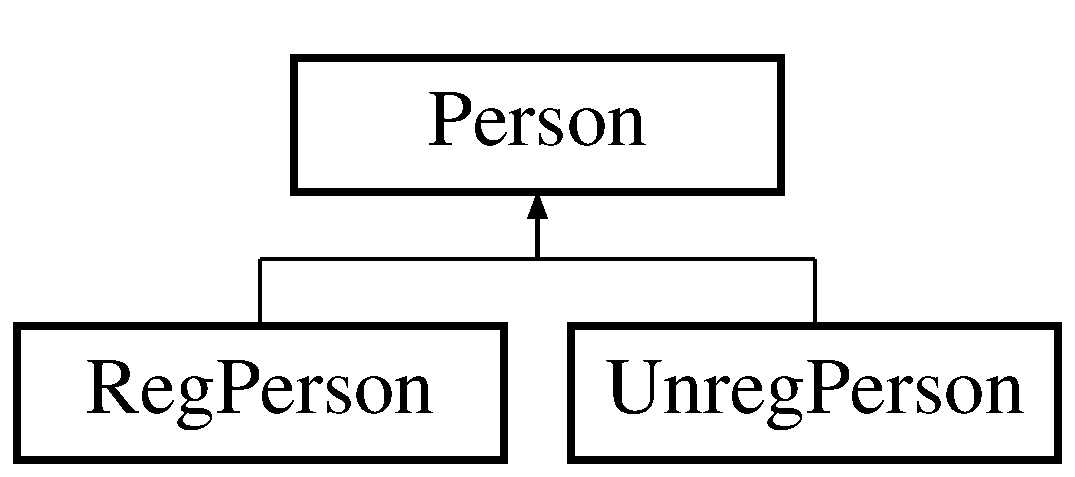
\includegraphics[height=2.000000cm]{class_person}
\end{center}
\end{figure}
\subsection*{Public Member Functions}
\begin{DoxyCompactItemize}
\item 
\hypertarget{class_person_a0397c6f89fafc12e738923f612bc41a3}{\hyperlink{class_person_a0397c6f89fafc12e738923f612bc41a3}{Person} ()}\label{class_person_a0397c6f89fafc12e738923f612bc41a3}

\begin{DoxyCompactList}\small\item\em \hyperlink{class_person}{Person} default constructor. \end{DoxyCompactList}\item 
\hyperlink{class_person_add253b6da1826be37fb9769eb2df2121}{Person} (string n, unsigned long t\+\_\+nr)
\begin{DoxyCompactList}\small\item\em \hyperlink{class_person}{Person} constructor. \end{DoxyCompactList}\item 
\hypertarget{class_person_a700ffd693321c5fe6880262acf43d4da}{virtual \hyperlink{class_person_a700ffd693321c5fe6880262acf43d4da}{$\sim$\+Person} ()}\label{class_person_a700ffd693321c5fe6880262acf43d4da}

\begin{DoxyCompactList}\small\item\em \hyperlink{class_person}{Person} destructor. \end{DoxyCompactList}\item 
void \hyperlink{class_person_a62b6b1cc2b0ce6dfa92786cfe2857362}{set\+Name} (string n)
\begin{DoxyCompactList}\small\item\em Sets the person's name. \end{DoxyCompactList}\item 
void \hyperlink{class_person_a7f178b2627a33e86c965bfaa0cc77ff0}{set\+Tel\+Nr} (unsigned long t\+\_\+nr)
\begin{DoxyCompactList}\small\item\em Sets the person's phone. \end{DoxyCompactList}\item 
void \hyperlink{class_person_ac52c35916ca323635f9b58cceaf7bfad}{set\+Billing} (float f)
\begin{DoxyCompactList}\small\item\em Sets the person's billing debt. \end{DoxyCompactList}\item 
string \hyperlink{class_person_a5c06a41731a2656caec65e3bc39f5ebe}{get\+Name} () const 
\begin{DoxyCompactList}\small\item\em Returns the name. \end{DoxyCompactList}\item 
unsigned long \hyperlink{class_person_a1b3237d0eba60fa12437ad8794729b16}{get\+Tel\+Nr} () const 
\begin{DoxyCompactList}\small\item\em Returns the phone. \end{DoxyCompactList}\item 
float \hyperlink{class_person_ad84e50825f66a2ab7f2571698f07cbbf}{get\+Billing} () const 
\begin{DoxyCompactList}\small\item\em Returns the billing debt. \end{DoxyCompactList}\item 
\hypertarget{class_person_a0dcd76e4e697490120f0c3417414c1a6}{void \hyperlink{class_person_a0dcd76e4e697490120f0c3417414c1a6}{pay\+Billing} ()}\label{class_person_a0dcd76e4e697490120f0c3417414c1a6}

\begin{DoxyCompactList}\small\item\em Outputs message that bill was paid, resets billing to 0. \end{DoxyCompactList}\end{DoxyCompactItemize}
\begin{Indent}{\bf Polymorphic functions}\par
\begin{DoxyCompactItemize}
\item 
\hypertarget{class_person_ab2e01c5852e65685b30c7f93af5a82e2}{virtual void {\bfseries add\+Bill} (string fee, float triplength)}\label{class_person_ab2e01c5852e65685b30c7f93af5a82e2}

\item 
\hypertarget{class_person_afe5e1da83f868d72cb9c49b371b066b4}{virtual void {\bfseries print\+Person} ()}\label{class_person_afe5e1da83f868d72cb9c49b371b066b4}

\item 
\hypertarget{class_person_a28b1defaeb5d84515f5c27674b2a3007}{virtual void {\bfseries add\+Trip\+History} (\hyperlink{class_trip}{Trip} $\ast$t)}\label{class_person_a28b1defaeb5d84515f5c27674b2a3007}

\item 
\hypertarget{class_person_a81e8251d01b54f58ae26e8dc18520eb1}{virtual string {\bfseries get\+Usern} () const }\label{class_person_a81e8251d01b54f58ae26e8dc18520eb1}

\end{DoxyCompactItemize}
\end{Indent}
\subsection*{Protected Attributes}
\begin{DoxyCompactItemize}
\item 
\hypertarget{class_person_a669b64897b4d823a27bb5866368d4dfa}{string {\bfseries name}}\label{class_person_a669b64897b4d823a27bb5866368d4dfa}

\item 
\hypertarget{class_person_a0118ba61947248bceca632314dc4ed64}{unsigned long {\bfseries telephone\+\_\+nr}}\label{class_person_a0118ba61947248bceca632314dc4ed64}

\item 
\hypertarget{class_person_ac9185a4fc1e41fc19b4a2059d000cb98}{float {\bfseries billing}}\label{class_person_ac9185a4fc1e41fc19b4a2059d000cb98}

\end{DoxyCompactItemize}


\subsection{Detailed Description}
\hyperlink{class_person}{Person} class. 

A generic person class, functions as superclass to \hyperlink{class_reg_person}{Reg\+Person} and \hyperlink{class_unreg_person}{Unreg\+Person} 

\subsection{Constructor \& Destructor Documentation}
\hypertarget{class_person_add253b6da1826be37fb9769eb2df2121}{\index{Person@{Person}!Person@{Person}}
\index{Person@{Person}!Person@{Person}}
\subsubsection[{Person}]{\setlength{\rightskip}{0pt plus 5cm}Person\+::\+Person (
\begin{DoxyParamCaption}
\item[{string}]{n, }
\item[{unsigned long}]{t\+\_\+nr}
\end{DoxyParamCaption}
)}}\label{class_person_add253b6da1826be37fb9769eb2df2121}


\hyperlink{class_person}{Person} constructor. 


\begin{DoxyParams}{Parameters}
{\em n} & person's name \\
\hline
{\em t\+\_\+nr} & person's phone \\
\hline
\end{DoxyParams}


\subsection{Member Function Documentation}
\hypertarget{class_person_ad84e50825f66a2ab7f2571698f07cbbf}{\index{Person@{Person}!get\+Billing@{get\+Billing}}
\index{get\+Billing@{get\+Billing}!Person@{Person}}
\subsubsection[{get\+Billing}]{\setlength{\rightskip}{0pt plus 5cm}float Person\+::get\+Billing (
\begin{DoxyParamCaption}
{}
\end{DoxyParamCaption}
) const}}\label{class_person_ad84e50825f66a2ab7f2571698f07cbbf}


Returns the billing debt. 

\begin{DoxyReturn}{Returns}
float with billing debt 
\end{DoxyReturn}
\hypertarget{class_person_a5c06a41731a2656caec65e3bc39f5ebe}{\index{Person@{Person}!get\+Name@{get\+Name}}
\index{get\+Name@{get\+Name}!Person@{Person}}
\subsubsection[{get\+Name}]{\setlength{\rightskip}{0pt plus 5cm}string Person\+::get\+Name (
\begin{DoxyParamCaption}
{}
\end{DoxyParamCaption}
) const}}\label{class_person_a5c06a41731a2656caec65e3bc39f5ebe}


Returns the name. 

\begin{DoxyReturn}{Returns}
string with the person's name 
\end{DoxyReturn}
\hypertarget{class_person_a1b3237d0eba60fa12437ad8794729b16}{\index{Person@{Person}!get\+Tel\+Nr@{get\+Tel\+Nr}}
\index{get\+Tel\+Nr@{get\+Tel\+Nr}!Person@{Person}}
\subsubsection[{get\+Tel\+Nr}]{\setlength{\rightskip}{0pt plus 5cm}unsigned long Person\+::get\+Tel\+Nr (
\begin{DoxyParamCaption}
{}
\end{DoxyParamCaption}
) const}}\label{class_person_a1b3237d0eba60fa12437ad8794729b16}


Returns the phone. 

\begin{DoxyReturn}{Returns}
long with the person's phone 
\end{DoxyReturn}
\hypertarget{class_person_ac52c35916ca323635f9b58cceaf7bfad}{\index{Person@{Person}!set\+Billing@{set\+Billing}}
\index{set\+Billing@{set\+Billing}!Person@{Person}}
\subsubsection[{set\+Billing}]{\setlength{\rightskip}{0pt plus 5cm}void Person\+::set\+Billing (
\begin{DoxyParamCaption}
\item[{float}]{f}
\end{DoxyParamCaption}
)}}\label{class_person_ac52c35916ca323635f9b58cceaf7bfad}


Sets the person's billing debt. 


\begin{DoxyParams}{Parameters}
{\em f} & float with wanted value \\
\hline
\end{DoxyParams}
\hypertarget{class_person_a62b6b1cc2b0ce6dfa92786cfe2857362}{\index{Person@{Person}!set\+Name@{set\+Name}}
\index{set\+Name@{set\+Name}!Person@{Person}}
\subsubsection[{set\+Name}]{\setlength{\rightskip}{0pt plus 5cm}void Person\+::set\+Name (
\begin{DoxyParamCaption}
\item[{string}]{n}
\end{DoxyParamCaption}
)}}\label{class_person_a62b6b1cc2b0ce6dfa92786cfe2857362}


Sets the person's name. 


\begin{DoxyParams}{Parameters}
{\em n} & string with the person's name \\
\hline
\end{DoxyParams}
\hypertarget{class_person_a7f178b2627a33e86c965bfaa0cc77ff0}{\index{Person@{Person}!set\+Tel\+Nr@{set\+Tel\+Nr}}
\index{set\+Tel\+Nr@{set\+Tel\+Nr}!Person@{Person}}
\subsubsection[{set\+Tel\+Nr}]{\setlength{\rightskip}{0pt plus 5cm}void Person\+::set\+Tel\+Nr (
\begin{DoxyParamCaption}
\item[{unsigned long}]{t\+\_\+nr}
\end{DoxyParamCaption}
)}}\label{class_person_a7f178b2627a33e86c965bfaa0cc77ff0}


Sets the person's phone. 


\begin{DoxyParams}{Parameters}
{\em t\+\_\+nr} & unsigned long with the person's phone \\
\hline
\end{DoxyParams}


The documentation for this class was generated from the following files\+:\begin{DoxyCompactItemize}
\item 
Person.\+h\item 
Person.\+cpp\end{DoxyCompactItemize}

\hypertarget{class_place}{\section{Place Class Reference}
\label{class_place}\index{Place@{Place}}
}


\hyperlink{class_place}{Place} class.  




{\ttfamily \#include $<$Place.\+h$>$}

\subsection*{Public Member Functions}
\begin{DoxyCompactItemize}
\item 
\hypertarget{class_place_ab5ae86c31e3a4c91800fb396d38e7a2b}{\hyperlink{class_place_ab5ae86c31e3a4c91800fb396d38e7a2b}{Place} ()}\label{class_place_ab5ae86c31e3a4c91800fb396d38e7a2b}

\begin{DoxyCompactList}\small\item\em \hyperlink{class_place}{Place} default constructor. \end{DoxyCompactList}\item 
\hyperlink{class_place_ae408c72c18378fea3139db133d8bf5a3}{Place} (string n, pair$<$ int, int $>$ coord)
\begin{DoxyCompactList}\small\item\em \hyperlink{class_place}{Place} constructor. \end{DoxyCompactList}\item 
\hypertarget{class_place_a190a59c6249d3b30d7ecfa8babe411ff}{\hyperlink{class_place_a190a59c6249d3b30d7ecfa8babe411ff}{$\sim$\+Place} ()}\label{class_place_a190a59c6249d3b30d7ecfa8babe411ff}

\begin{DoxyCompactList}\small\item\em \hyperlink{class_place}{Place} destructor. \end{DoxyCompactList}\item 
void \hyperlink{class_place_a6dcfdcda0a20a4d747b9b5657fc0e627}{set\+Name} (string n)
\begin{DoxyCompactList}\small\item\em Sets the place's name. \end{DoxyCompactList}\item 
void \hyperlink{class_place_ad5b15f3ca8aef6b51e0b6958ba40e106}{set\+Coords} (int x, int y)
\begin{DoxyCompactList}\small\item\em Sets the place's coordinates. \end{DoxyCompactList}\item 
string \hyperlink{class_place_a9353ceaa630511ca25a133cc545f6b93}{get\+Name} () const 
\begin{DoxyCompactList}\small\item\em Returns the name of the place. \end{DoxyCompactList}\item 
pair$<$ int, int $>$ \hyperlink{class_place_adf486c33d5463f1b0000a286cc171beb}{get\+Coords} () const 
\begin{DoxyCompactList}\small\item\em Returns the place's coordinates. \end{DoxyCompactList}\item 
string \hyperlink{class_place_af3d96742c03650c51726c5dde5ba0dd5}{to\+String} ()
\begin{DoxyCompactList}\small\item\em Writes all the information about a place to a string. \end{DoxyCompactList}\end{DoxyCompactItemize}


\subsection{Detailed Description}
\hyperlink{class_place}{Place} class. 

Contains the place related functions, including getters, setters and to\+String functions. 

\subsection{Constructor \& Destructor Documentation}
\hypertarget{class_place_ae408c72c18378fea3139db133d8bf5a3}{\index{Place@{Place}!Place@{Place}}
\index{Place@{Place}!Place@{Place}}
\subsubsection[{Place}]{\setlength{\rightskip}{0pt plus 5cm}Place\+::\+Place (
\begin{DoxyParamCaption}
\item[{string}]{n, }
\item[{pair$<$ int, int $>$}]{coords}
\end{DoxyParamCaption}
)}}\label{class_place_ae408c72c18378fea3139db133d8bf5a3}


\hyperlink{class_place}{Place} constructor. 


\begin{DoxyParams}{Parameters}
{\em n} & name of the place \\
\hline
{\em coord} & place's coordinates \\
\hline
\end{DoxyParams}


\subsection{Member Function Documentation}
\hypertarget{class_place_adf486c33d5463f1b0000a286cc171beb}{\index{Place@{Place}!get\+Coords@{get\+Coords}}
\index{get\+Coords@{get\+Coords}!Place@{Place}}
\subsubsection[{get\+Coords}]{\setlength{\rightskip}{0pt plus 5cm}pair$<$ int, int $>$ Place\+::get\+Coords (
\begin{DoxyParamCaption}
{}
\end{DoxyParamCaption}
) const}}\label{class_place_adf486c33d5463f1b0000a286cc171beb}


Returns the place's coordinates. 

\begin{DoxyReturn}{Returns}
pair$<$int,int$>$ with the place's coordinates 
\end{DoxyReturn}
\hypertarget{class_place_a9353ceaa630511ca25a133cc545f6b93}{\index{Place@{Place}!get\+Name@{get\+Name}}
\index{get\+Name@{get\+Name}!Place@{Place}}
\subsubsection[{get\+Name}]{\setlength{\rightskip}{0pt plus 5cm}string Place\+::get\+Name (
\begin{DoxyParamCaption}
{}
\end{DoxyParamCaption}
) const}}\label{class_place_a9353ceaa630511ca25a133cc545f6b93}


Returns the name of the place. 

\begin{DoxyReturn}{Returns}
string with the place's name 
\end{DoxyReturn}
\hypertarget{class_place_ad5b15f3ca8aef6b51e0b6958ba40e106}{\index{Place@{Place}!set\+Coords@{set\+Coords}}
\index{set\+Coords@{set\+Coords}!Place@{Place}}
\subsubsection[{set\+Coords}]{\setlength{\rightskip}{0pt plus 5cm}void Place\+::set\+Coords (
\begin{DoxyParamCaption}
\item[{int}]{x, }
\item[{int}]{y}
\end{DoxyParamCaption}
)}}\label{class_place_ad5b15f3ca8aef6b51e0b6958ba40e106}


Sets the place's coordinates. 


\begin{DoxyParams}{Parameters}
{\em int} & x coordinate in x axis \\
\hline
{\em int} & y coordinate in y axis \\
\hline
\end{DoxyParams}
\hypertarget{class_place_a6dcfdcda0a20a4d747b9b5657fc0e627}{\index{Place@{Place}!set\+Name@{set\+Name}}
\index{set\+Name@{set\+Name}!Place@{Place}}
\subsubsection[{set\+Name}]{\setlength{\rightskip}{0pt plus 5cm}void Place\+::set\+Name (
\begin{DoxyParamCaption}
\item[{string}]{n}
\end{DoxyParamCaption}
)}}\label{class_place_a6dcfdcda0a20a4d747b9b5657fc0e627}


Sets the place's name. 


\begin{DoxyParams}{Parameters}
{\em n} & string with the place's name \\
\hline
\end{DoxyParams}
\hypertarget{class_place_af3d96742c03650c51726c5dde5ba0dd5}{\index{Place@{Place}!to\+String@{to\+String}}
\index{to\+String@{to\+String}!Place@{Place}}
\subsubsection[{to\+String}]{\setlength{\rightskip}{0pt plus 5cm}string Place\+::to\+String (
\begin{DoxyParamCaption}
{}
\end{DoxyParamCaption}
)}}\label{class_place_af3d96742c03650c51726c5dde5ba0dd5}


Writes all the information about a place to a string. 

\begin{DoxyReturn}{Returns}
string with the place's information 
\end{DoxyReturn}


The documentation for this class was generated from the following files\+:\begin{DoxyCompactItemize}
\item 
Place.\+h\item 
Place.\+cpp\end{DoxyCompactItemize}

\hypertarget{class_reg_person}{\section{Reg\+Person Class Reference}
\label{class_reg_person}\index{Reg\+Person@{Reg\+Person}}
}


\hyperlink{class_unreg_person}{Unreg\+Person} class.  




{\ttfamily \#include $<$Person.\+h$>$}

Inheritance diagram for Reg\+Person\+:\begin{figure}[H]
\begin{center}
\leavevmode
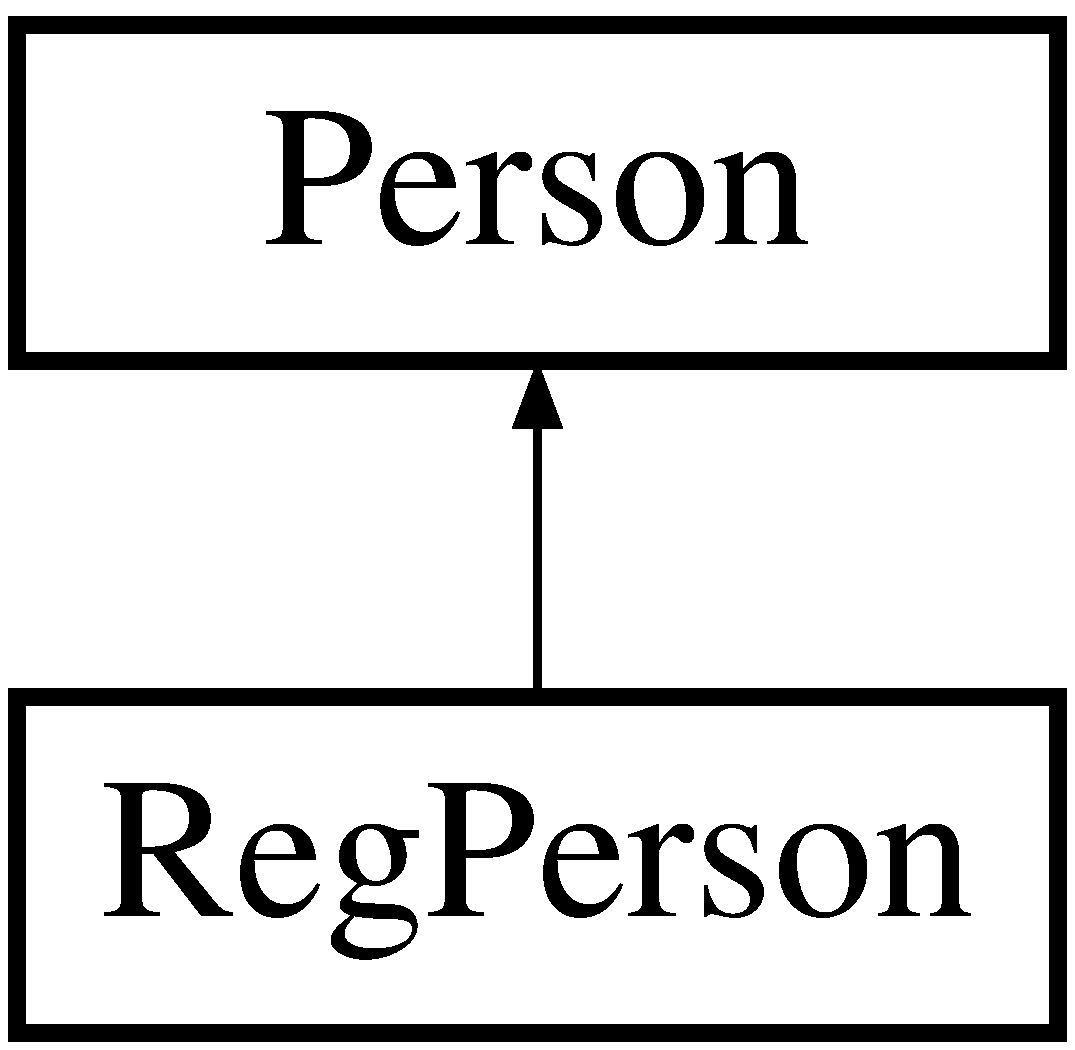
\includegraphics[height=2.000000cm]{class_reg_person}
\end{center}
\end{figure}
\subsection*{Public Member Functions}
\begin{DoxyCompactItemize}
\item 
\hypertarget{class_reg_person_a607b780b62f25aba32b0b1292949e8d8}{\hyperlink{class_reg_person_a607b780b62f25aba32b0b1292949e8d8}{Reg\+Person} ()}\label{class_reg_person_a607b780b62f25aba32b0b1292949e8d8}

\begin{DoxyCompactList}\small\item\em \hyperlink{class_reg_person}{Reg\+Person} default constructor. \end{DoxyCompactList}\item 
\hyperlink{class_reg_person_aa584be9f308b5f0257817ac9b015c1b4}{Reg\+Person} (string n, unsigned long t\+\_\+nr, string uname, string passw)
\begin{DoxyCompactList}\small\item\em \hyperlink{class_reg_person}{Reg\+Person} constructor. \end{DoxyCompactList}\item 
\hypertarget{class_reg_person_acc2f3a1c7f87cbb947f76642b0208b62}{\hyperlink{class_reg_person_acc2f3a1c7f87cbb947f76642b0208b62}{$\sim$\+Reg\+Person} ()}\label{class_reg_person_acc2f3a1c7f87cbb947f76642b0208b62}

\begin{DoxyCompactList}\small\item\em \hyperlink{class_reg_person}{Reg\+Person} destructor. \end{DoxyCompactList}\item 
\hypertarget{class_reg_person_abd22f72e4d87ce17c58e0b674160285e}{void \hyperlink{class_reg_person_abd22f72e4d87ce17c58e0b674160285e}{set\+Passw} (string pw)}\label{class_reg_person_abd22f72e4d87ce17c58e0b674160285e}

\begin{DoxyCompactList}\small\item\em Sets password to pw. \end{DoxyCompactList}\item 
\hypertarget{class_reg_person_a6a67d8f2dc03110d57f475e17ee330d8}{void \hyperlink{class_reg_person_a6a67d8f2dc03110d57f475e17ee330d8}{set\+Usern} (string usrn)}\label{class_reg_person_a6a67d8f2dc03110d57f475e17ee330d8}

\begin{DoxyCompactList}\small\item\em Sets username to usrn. \end{DoxyCompactList}\item 
string \hyperlink{class_reg_person_a3b2b617680af61b9af7fac6a4d2a69fb}{get\+Passw} () const 
\begin{DoxyCompactList}\small\item\em Returns the password. \end{DoxyCompactList}\item 
string \hyperlink{class_reg_person_ab2ea80db160779902c00c65e07249d18}{get\+Usern} () const 
\begin{DoxyCompactList}\small\item\em Returns the username. \end{DoxyCompactList}\item 
bool \hyperlink{class_reg_person_ae1c37bdaecf7775c657680e10d5819cc}{get\+Has\+Vehicle} () const 
\begin{DoxyCompactList}\small\item\em check if user has vehicles \end{DoxyCompactList}\item 
vector$<$ \hyperlink{class_reg_person}{Reg\+Person} $\ast$ $>$ \& \hyperlink{class_reg_person_a498a20eb4a5869a3a4d4266ec76a2356}{get\+Buddies} ()
\begin{DoxyCompactList}\small\item\em returns buddies \end{DoxyCompactList}\item 
vector$<$ \hyperlink{class_vehicle}{Vehicle} $\ast$ $>$ \& \hyperlink{class_reg_person_ae1ef0364b2731ddd51460a3c37054457}{get\+Vehicles} ()
\begin{DoxyCompactList}\small\item\em returns vehicles \end{DoxyCompactList}\item 
vector$<$ string $>$ \& \hyperlink{class_reg_person_a523aef12cf566320a97d19f6dcc15a11}{get\+Notifications} ()
\begin{DoxyCompactList}\small\item\em get user notifications \end{DoxyCompactList}\item 
vector$<$ \hyperlink{class_trip}{Trip} $\ast$ $>$ \& \hyperlink{class_reg_person_a352a761ffdd5f3bd9f0a4c10538789a6}{get\+Trip\+History} ()
\begin{DoxyCompactList}\small\item\em get user trip history \end{DoxyCompactList}\item 
void \hyperlink{class_reg_person_ab3aceab8edc0a7a68dcb56184709cea3}{insert\+Buddy} (\hyperlink{class_reg_person}{Reg\+Person} $\ast$other\+\_\+person)
\begin{DoxyCompactList}\small\item\em Add other\+\_\+person to user's buddy vector. \end{DoxyCompactList}\item 
void \hyperlink{class_reg_person_af84c947ee794a662d27b6437edfb16f5}{remove\+Buddy} (int index)
\begin{DoxyCompactList}\small\item\em Remove a buddy from vector. \end{DoxyCompactList}\item 
\hypertarget{class_reg_person_ac3ba518d24465719eb3e10ab8689d380}{void \hyperlink{class_reg_person_ac3ba518d24465719eb3e10ab8689d380}{add\+Trip\+History} (\hyperlink{class_trip}{Trip} $\ast$t)}\label{class_reg_person_ac3ba518d24465719eb3e10ab8689d380}

\begin{DoxyCompactList}\small\item\em Add a trip to trip history vector. \end{DoxyCompactList}\item 
void \hyperlink{class_reg_person_a1e4f00c8000681e45b95bbf8b91e2e98}{add\+Vehicle} (\hyperlink{class_vehicle}{Vehicle} $\ast$v)
\begin{DoxyCompactList}\small\item\em Add vehicle to user's vehicle vector. \end{DoxyCompactList}\item 
void \hyperlink{class_reg_person_afa8a8ed022555e8b0c780712627f5c25}{remove\+Vehicle} (int index)
\begin{DoxyCompactList}\small\item\em Remove a vehicle from vector. \end{DoxyCompactList}\item 
bool \hyperlink{class_reg_person_a33a4f3d04487aa4857a791d82e967e98}{are\+Mutual\+Buddies} (\hyperlink{class_reg_person}{Reg\+Person} $\ast$other\+\_\+person) const 
\begin{DoxyCompactList}\small\item\em check if user is mutual buddy with other person \end{DoxyCompactList}\item 
\hypertarget{class_reg_person_a7ad9eadc18f0f9492c3bcaca195bd08d}{void \hyperlink{class_reg_person_a7ad9eadc18f0f9492c3bcaca195bd08d}{add\+Notifications} (string message)}\label{class_reg_person_a7ad9eadc18f0f9492c3bcaca195bd08d}

\begin{DoxyCompactList}\small\item\em Add message to notifications vector. \end{DoxyCompactList}\item 
void \hyperlink{class_reg_person_a5013a9edcbfd91a172f94a5c6a707442}{show\+Notifications} (int howmany)
\begin{DoxyCompactList}\small\item\em Displays specified number of notifications. \end{DoxyCompactList}\item 
void \hyperlink{class_reg_person_a79fe3960ee3518cca16a94535852b2c1}{add\+Bill} (string fee, float triplength)
\begin{DoxyCompactList}\small\item\em Adds bill to billing, if user has vehicles, trips are free of charge. \end{DoxyCompactList}\item 
\hypertarget{class_reg_person_a83b75667247384c8f2e083ca17f095e0}{void \hyperlink{class_reg_person_a83b75667247384c8f2e083ca17f095e0}{print\+Person} ()}\label{class_reg_person_a83b75667247384c8f2e083ca17f095e0}

\begin{DoxyCompactList}\small\item\em Prints registered person's information. \end{DoxyCompactList}\item 
\hypertarget{class_reg_person_a3daa5293f513d5b7a30477a044d3ff6f}{void \hyperlink{class_reg_person_a3daa5293f513d5b7a30477a044d3ff6f}{print\+Trip\+History} ()}\label{class_reg_person_a3daa5293f513d5b7a30477a044d3ff6f}

\begin{DoxyCompactList}\small\item\em prints the vector of trip history of user \end{DoxyCompactList}\end{DoxyCompactItemize}
\subsection*{Additional Inherited Members}


\subsection{Detailed Description}
\hyperlink{class_unreg_person}{Unreg\+Person} class. 

\hyperlink{class_person}{Person} subclass, represents registered users in the application 

\subsection{Constructor \& Destructor Documentation}
\hypertarget{class_reg_person_aa584be9f308b5f0257817ac9b015c1b4}{\index{Reg\+Person@{Reg\+Person}!Reg\+Person@{Reg\+Person}}
\index{Reg\+Person@{Reg\+Person}!Reg\+Person@{Reg\+Person}}
\subsubsection[{Reg\+Person}]{\setlength{\rightskip}{0pt plus 5cm}Reg\+Person\+::\+Reg\+Person (
\begin{DoxyParamCaption}
\item[{string}]{n, }
\item[{unsigned long}]{t\+\_\+nr, }
\item[{string}]{uname, }
\item[{string}]{passw}
\end{DoxyParamCaption}
)}}\label{class_reg_person_aa584be9f308b5f0257817ac9b015c1b4}


\hyperlink{class_reg_person}{Reg\+Person} constructor. 


\begin{DoxyParams}{Parameters}
{\em n} & person's name \\
\hline
{\em t\+\_\+nr} & person's phone \\
\hline
{\em uname} & person's username \\
\hline
{\em passw} & person's password \\
\hline
\end{DoxyParams}


\subsection{Member Function Documentation}
\hypertarget{class_reg_person_a79fe3960ee3518cca16a94535852b2c1}{\index{Reg\+Person@{Reg\+Person}!add\+Bill@{add\+Bill}}
\index{add\+Bill@{add\+Bill}!Reg\+Person@{Reg\+Person}}
\subsubsection[{add\+Bill}]{\setlength{\rightskip}{0pt plus 5cm}void Reg\+Person\+::add\+Bill (
\begin{DoxyParamCaption}
\item[{string}]{fee, }
\item[{float}]{triplength}
\end{DoxyParamCaption}
)\hspace{0.3cm}{\ttfamily [virtual]}}}\label{class_reg_person_a79fe3960ee3518cca16a94535852b2c1}


Adds bill to billing, if user has vehicles, trips are free of charge. 


\begin{DoxyParams}{Parameters}
{\em string} & fee -\/ what kind of fee to charge \\
\hline
{\em float} & triplength -\/ distance of the trip produces higher charges \\
\hline
\end{DoxyParams}


Reimplemented from \hyperlink{class_person}{Person}.

\hypertarget{class_reg_person_a1e4f00c8000681e45b95bbf8b91e2e98}{\index{Reg\+Person@{Reg\+Person}!add\+Vehicle@{add\+Vehicle}}
\index{add\+Vehicle@{add\+Vehicle}!Reg\+Person@{Reg\+Person}}
\subsubsection[{add\+Vehicle}]{\setlength{\rightskip}{0pt plus 5cm}void Reg\+Person\+::add\+Vehicle (
\begin{DoxyParamCaption}
\item[{{\bf Vehicle} $\ast$}]{v}
\end{DoxyParamCaption}
)}}\label{class_reg_person_a1e4f00c8000681e45b95bbf8b91e2e98}


Add vehicle to user's vehicle vector. 


\begin{DoxyParams}{Parameters}
{\em \hyperlink{class_vehicle}{Vehicle}} & $\ast$ v -\/ vehicle to add \\
\hline
\end{DoxyParams}
\hypertarget{class_reg_person_a33a4f3d04487aa4857a791d82e967e98}{\index{Reg\+Person@{Reg\+Person}!are\+Mutual\+Buddies@{are\+Mutual\+Buddies}}
\index{are\+Mutual\+Buddies@{are\+Mutual\+Buddies}!Reg\+Person@{Reg\+Person}}
\subsubsection[{are\+Mutual\+Buddies}]{\setlength{\rightskip}{0pt plus 5cm}bool Reg\+Person\+::are\+Mutual\+Buddies (
\begin{DoxyParamCaption}
\item[{{\bf Reg\+Person} $\ast$}]{other\+\_\+person}
\end{DoxyParamCaption}
) const}}\label{class_reg_person_a33a4f3d04487aa4857a791d82e967e98}


check if user is mutual buddy with other person 

\begin{DoxyReturn}{Returns}
bool true if mutual buddies, false otherwise 
\end{DoxyReturn}
\hypertarget{class_reg_person_a498a20eb4a5869a3a4d4266ec76a2356}{\index{Reg\+Person@{Reg\+Person}!get\+Buddies@{get\+Buddies}}
\index{get\+Buddies@{get\+Buddies}!Reg\+Person@{Reg\+Person}}
\subsubsection[{get\+Buddies}]{\setlength{\rightskip}{0pt plus 5cm}vector$<$ {\bf Reg\+Person} $\ast$ $>$ \& Reg\+Person\+::get\+Buddies (
\begin{DoxyParamCaption}
{}
\end{DoxyParamCaption}
)}}\label{class_reg_person_a498a20eb4a5869a3a4d4266ec76a2356}


returns buddies 

\begin{DoxyReturn}{Returns}
vector of buddies 
\end{DoxyReturn}
\hypertarget{class_reg_person_ae1c37bdaecf7775c657680e10d5819cc}{\index{Reg\+Person@{Reg\+Person}!get\+Has\+Vehicle@{get\+Has\+Vehicle}}
\index{get\+Has\+Vehicle@{get\+Has\+Vehicle}!Reg\+Person@{Reg\+Person}}
\subsubsection[{get\+Has\+Vehicle}]{\setlength{\rightskip}{0pt plus 5cm}bool Reg\+Person\+::get\+Has\+Vehicle (
\begin{DoxyParamCaption}
{}
\end{DoxyParamCaption}
) const}}\label{class_reg_person_ae1c37bdaecf7775c657680e10d5819cc}


check if user has vehicles 

\begin{DoxyReturn}{Returns}
bool true if he has vehicles, false otherwise 
\end{DoxyReturn}
\hypertarget{class_reg_person_a523aef12cf566320a97d19f6dcc15a11}{\index{Reg\+Person@{Reg\+Person}!get\+Notifications@{get\+Notifications}}
\index{get\+Notifications@{get\+Notifications}!Reg\+Person@{Reg\+Person}}
\subsubsection[{get\+Notifications}]{\setlength{\rightskip}{0pt plus 5cm}vector$<$ string $>$ \& Reg\+Person\+::get\+Notifications (
\begin{DoxyParamCaption}
{}
\end{DoxyParamCaption}
)}}\label{class_reg_person_a523aef12cf566320a97d19f6dcc15a11}


get user notifications 

\begin{DoxyReturn}{Returns}
return the vector of strings with notifications 
\end{DoxyReturn}
\hypertarget{class_reg_person_a3b2b617680af61b9af7fac6a4d2a69fb}{\index{Reg\+Person@{Reg\+Person}!get\+Passw@{get\+Passw}}
\index{get\+Passw@{get\+Passw}!Reg\+Person@{Reg\+Person}}
\subsubsection[{get\+Passw}]{\setlength{\rightskip}{0pt plus 5cm}string Reg\+Person\+::get\+Passw (
\begin{DoxyParamCaption}
{}
\end{DoxyParamCaption}
) const}}\label{class_reg_person_a3b2b617680af61b9af7fac6a4d2a69fb}


Returns the password. 

\begin{DoxyReturn}{Returns}
string with password 
\end{DoxyReturn}
\hypertarget{class_reg_person_a352a761ffdd5f3bd9f0a4c10538789a6}{\index{Reg\+Person@{Reg\+Person}!get\+Trip\+History@{get\+Trip\+History}}
\index{get\+Trip\+History@{get\+Trip\+History}!Reg\+Person@{Reg\+Person}}
\subsubsection[{get\+Trip\+History}]{\setlength{\rightskip}{0pt plus 5cm}vector$<$ {\bf Trip} $\ast$ $>$ \& Reg\+Person\+::get\+Trip\+History (
\begin{DoxyParamCaption}
{}
\end{DoxyParamCaption}
)}}\label{class_reg_person_a352a761ffdd5f3bd9f0a4c10538789a6}


get user trip history 

\begin{DoxyReturn}{Returns}
returns vector of trips 
\end{DoxyReturn}
\hypertarget{class_reg_person_ab2ea80db160779902c00c65e07249d18}{\index{Reg\+Person@{Reg\+Person}!get\+Usern@{get\+Usern}}
\index{get\+Usern@{get\+Usern}!Reg\+Person@{Reg\+Person}}
\subsubsection[{get\+Usern}]{\setlength{\rightskip}{0pt plus 5cm}string Reg\+Person\+::get\+Usern (
\begin{DoxyParamCaption}
{}
\end{DoxyParamCaption}
) const\hspace{0.3cm}{\ttfamily [virtual]}}}\label{class_reg_person_ab2ea80db160779902c00c65e07249d18}


Returns the username. 

\begin{DoxyReturn}{Returns}
string with username 
\end{DoxyReturn}


Reimplemented from \hyperlink{class_person}{Person}.

\hypertarget{class_reg_person_ae1ef0364b2731ddd51460a3c37054457}{\index{Reg\+Person@{Reg\+Person}!get\+Vehicles@{get\+Vehicles}}
\index{get\+Vehicles@{get\+Vehicles}!Reg\+Person@{Reg\+Person}}
\subsubsection[{get\+Vehicles}]{\setlength{\rightskip}{0pt plus 5cm}vector$<$ {\bf Vehicle} $\ast$ $>$ \& Reg\+Person\+::get\+Vehicles (
\begin{DoxyParamCaption}
{}
\end{DoxyParamCaption}
)}}\label{class_reg_person_ae1ef0364b2731ddd51460a3c37054457}


returns vehicles 

\begin{DoxyReturn}{Returns}
vector of vehicles 
\end{DoxyReturn}
\hypertarget{class_reg_person_ab3aceab8edc0a7a68dcb56184709cea3}{\index{Reg\+Person@{Reg\+Person}!insert\+Buddy@{insert\+Buddy}}
\index{insert\+Buddy@{insert\+Buddy}!Reg\+Person@{Reg\+Person}}
\subsubsection[{insert\+Buddy}]{\setlength{\rightskip}{0pt plus 5cm}void Reg\+Person\+::insert\+Buddy (
\begin{DoxyParamCaption}
\item[{{\bf Reg\+Person} $\ast$}]{other\+\_\+person}
\end{DoxyParamCaption}
)}}\label{class_reg_person_ab3aceab8edc0a7a68dcb56184709cea3}


Add other\+\_\+person to user's buddy vector. 


\begin{DoxyParams}{Parameters}
{\em Reg\+Person$\ast$} & other\+\_\+person -\/ buddy to add \\
\hline
\end{DoxyParams}
\hypertarget{class_reg_person_af84c947ee794a662d27b6437edfb16f5}{\index{Reg\+Person@{Reg\+Person}!remove\+Buddy@{remove\+Buddy}}
\index{remove\+Buddy@{remove\+Buddy}!Reg\+Person@{Reg\+Person}}
\subsubsection[{remove\+Buddy}]{\setlength{\rightskip}{0pt plus 5cm}void Reg\+Person\+::remove\+Buddy (
\begin{DoxyParamCaption}
\item[{int}]{index}
\end{DoxyParamCaption}
)}}\label{class_reg_person_af84c947ee794a662d27b6437edfb16f5}


Remove a buddy from vector. 


\begin{DoxyParams}{Parameters}
{\em int} & index -\/ index of buddy to delete from vector \\
\hline
\end{DoxyParams}
\hypertarget{class_reg_person_afa8a8ed022555e8b0c780712627f5c25}{\index{Reg\+Person@{Reg\+Person}!remove\+Vehicle@{remove\+Vehicle}}
\index{remove\+Vehicle@{remove\+Vehicle}!Reg\+Person@{Reg\+Person}}
\subsubsection[{remove\+Vehicle}]{\setlength{\rightskip}{0pt plus 5cm}void Reg\+Person\+::remove\+Vehicle (
\begin{DoxyParamCaption}
\item[{int}]{index}
\end{DoxyParamCaption}
)}}\label{class_reg_person_afa8a8ed022555e8b0c780712627f5c25}


Remove a vehicle from vector. 


\begin{DoxyParams}{Parameters}
{\em int} & index -\/ index of vehicle to delete from vector \\
\hline
\end{DoxyParams}
\hypertarget{class_reg_person_a5013a9edcbfd91a172f94a5c6a707442}{\index{Reg\+Person@{Reg\+Person}!show\+Notifications@{show\+Notifications}}
\index{show\+Notifications@{show\+Notifications}!Reg\+Person@{Reg\+Person}}
\subsubsection[{show\+Notifications}]{\setlength{\rightskip}{0pt plus 5cm}void Reg\+Person\+::show\+Notifications (
\begin{DoxyParamCaption}
\item[{int}]{howmany}
\end{DoxyParamCaption}
)}}\label{class_reg_person_a5013a9edcbfd91a172f94a5c6a707442}


Displays specified number of notifications. 


\begin{DoxyParams}{Parameters}
{\em int} & howmany -\/ number of notifications to display \\
\hline
\end{DoxyParams}


The documentation for this class was generated from the following files\+:\begin{DoxyCompactItemize}
\item 
Person.\+h\item 
Person.\+cpp\end{DoxyCompactItemize}

\hypertarget{class_save_failed}{\section{Save\+Failed Class Reference}
\label{class_save_failed}\index{Save\+Failed@{Save\+Failed}}
}


The documentation for this class was generated from the following file\+:\begin{DoxyCompactItemize}
\item 
Logic.\+h\end{DoxyCompactItemize}

\hypertarget{class_trip}{\section{Trip Class Reference}
\label{class_trip}\index{Trip@{Trip}}
}


\hyperlink{class_trip}{Trip} class Contains all of the trip related functions, including getters, setters and C\+R\+U\+D functions.  




{\ttfamily \#include $<$Trip.\+h$>$}

\subsection*{Public Member Functions}
\begin{DoxyCompactItemize}
\item 
\hypertarget{class_trip_aa67b77d0d2de622ed5eb9e9cad34db8f}{\hyperlink{class_trip_aa67b77d0d2de622ed5eb9e9cad34db8f}{Trip} ()}\label{class_trip_aa67b77d0d2de622ed5eb9e9cad34db8f}

\begin{DoxyCompactList}\small\item\em \hyperlink{class_trip}{Trip} default constructor. \end{DoxyCompactList}\item 
\hyperlink{class_trip_a0d0fce19644be21e8baec31492ad58fa}{Trip} (string Vehicle\+Owner, \hyperlink{class_vehicle}{Vehicle} $\ast$vehicle, bool smoke, \hyperlink{class_date}{Date} s, \hyperlink{class_date}{Date} e)
\begin{DoxyCompactList}\small\item\em \hyperlink{class_trip}{Trip} constructor. \end{DoxyCompactList}\item 
\hyperlink{class_trip_a71b15d051b75c1d1eee38a5c38191920}{Trip} (string Vehicle\+Owner, unsigned int seats, bool smoke, \hyperlink{class_date}{Date} s, \hyperlink{class_date}{Date} e)
\begin{DoxyCompactList}\small\item\em \hyperlink{class_trip}{Trip} constructor. \end{DoxyCompactList}\item 
\hypertarget{class_trip_a2376daed3b03469163782ef0d0533d52}{\hyperlink{class_trip_a2376daed3b03469163782ef0d0533d52}{$\sim$\+Trip} ()}\label{class_trip_a2376daed3b03469163782ef0d0533d52}

\begin{DoxyCompactList}\small\item\em \hyperlink{class_trip}{Trip} default destructor. \end{DoxyCompactList}\item 
unsigned int \hyperlink{class_trip_a48282720f54aa5d56d5ba872868396e6}{get\+Available\+Seats} () const 
\begin{DoxyCompactList}\small\item\em Returns the number of available seats in the trip. \end{DoxyCompactList}\item 
float \hyperlink{class_trip_a40b102c05b9f11486affb653d289503a}{get\+Distance} () const 
\begin{DoxyCompactList}\small\item\em Returns the trip's distance. \end{DoxyCompactList}\item 
vector$<$ pair$<$ \hyperlink{class_place}{Place} $\ast$, int $>$ $>$ \hyperlink{class_trip_a4b1a35b6c36433ce982d7a42b6df796d}{get\+Route} () const 
\begin{DoxyCompactList}\small\item\em Returns the trip's route. \end{DoxyCompactList}\item 
bool \hyperlink{class_trip_a842bbff21be74ba2dbd121728b383653}{get\+Smoking\+Sign} () const 
\begin{DoxyCompactList}\small\item\em Returns if the trip allows smoking. \end{DoxyCompactList}\item 
\hyperlink{class_date}{Date} \hyperlink{class_trip_af48effa8c9d9ff4b8e2e0ff5225d6f60}{get\+Start} () const 
\begin{DoxyCompactList}\small\item\em Returns the trip's start date. \end{DoxyCompactList}\item 
\hyperlink{class_date}{Date} \hyperlink{class_trip_a254a9341368c276926164e0d2cee4748}{get\+End} () const 
\begin{DoxyCompactList}\small\item\em Returns the trip's end date. \end{DoxyCompactList}\item 
\hypertarget{class_trip_a6e2a07b62197450f6e7158d1c3b882bb}{vector$<$ \hyperlink{class_person}{Person} $\ast$ $>$ \& {\bfseries get\+Travellers} ()}\label{class_trip_a6e2a07b62197450f6e7158d1c3b882bb}

\item 
string \hyperlink{class_trip_add7c86d5ee780f49b44df1d936229687}{get\+Driver} () const 
\begin{DoxyCompactList}\small\item\em Returns the name of the driver. \end{DoxyCompactList}\item 
\hyperlink{class_vehicle}{Vehicle} $\ast$ \hyperlink{class_trip_a7a2776544c9600f2e6a355e04f17e67b}{get\+Vehicle} () const 
\begin{DoxyCompactList}\small\item\em Returns the vehicle used in the trip. \end{DoxyCompactList}\item 
void \hyperlink{class_trip_a0166bf54e1fab842e494615041fb5bcd}{set\+Available\+Seats} (unsigned int a\+\_\+s)
\begin{DoxyCompactList}\small\item\em Sets the trip's available seats. \end{DoxyCompactList}\item 
void \hyperlink{class_trip_a011f6b53b9bdaf4f08106362fe0e391b}{set\+Vehicle} (\hyperlink{class_vehicle}{Vehicle} $\ast$v)
\begin{DoxyCompactList}\small\item\em Sets the trip's vehicle. \end{DoxyCompactList}\item 
void \hyperlink{class_trip_a17637add14f81f30c8f59f5812da2232}{set\+Distance} (float d)
\begin{DoxyCompactList}\small\item\em Sets the trip's distance. \end{DoxyCompactList}\item 
void \hyperlink{class_trip_a1df5fa0bd340a624e732c9452b62b4cb}{set\+Smoking\+Sign} (bool s)
\begin{DoxyCompactList}\small\item\em Sets the trip's distance. \end{DoxyCompactList}\item 
void \hyperlink{class_trip_a45b53f2a30771184c7a8491453cfa3da}{set\+Start} (\hyperlink{class_date}{Date} s)
\begin{DoxyCompactList}\small\item\em Sets the trip's start date. \end{DoxyCompactList}\item 
void \hyperlink{class_trip_a3d1b06fb96cbffd00cf16b4fe8ea1331}{set\+End} (\hyperlink{class_date}{Date} e)
\begin{DoxyCompactList}\small\item\em Sets the trip's end date. \end{DoxyCompactList}\item 
void \hyperlink{class_trip_adae7ef5a06244525d607f96bee531c49}{add\+Route} (vector$<$ pair$<$ \hyperlink{class_place}{Place} $\ast$, int $>$ $>$ rota)
\begin{DoxyCompactList}\small\item\em sets a route to the trip and the corresponding distance \end{DoxyCompactList}\item 
void \hyperlink{class_trip_a670b6fd9f234cb0448bc72454f0e546d}{add\+Traveller} (\hyperlink{class_person}{Person} $\ast$t, vector$<$ \hyperlink{class_place}{Place} $\ast$ $>$)
\begin{DoxyCompactList}\small\item\em adds a traveller to a trip, recalculates the number of available seats \end{DoxyCompactList}\item 
void \hyperlink{class_trip_ad3f71fd3cc8c5adeb9fc19779725081e}{remove\+Traveller} (\hyperlink{class_person}{Person} $\ast$t)
\begin{DoxyCompactList}\small\item\em removes a traveller from a trip, recalculates the number of available seats \end{DoxyCompactList}\item 
void \hyperlink{class_trip_a2d345864b78ff8ad01af06a981f1443b}{update\+Traveller\+Route} (\hyperlink{class_person}{Person} $\ast$t, vector$<$ \hyperlink{class_place}{Place} $\ast$ $>$r)
\begin{DoxyCompactList}\small\item\em updates a traveller's trip \end{DoxyCompactList}\item 
bool \hyperlink{class_trip_a96a633cf3d950759c6734041efc8fe8e}{is\+Traveller} (\hyperlink{class_person}{Person} $\ast$p)
\begin{DoxyCompactList}\small\item\em Checks if a person is a traveller. \end{DoxyCompactList}\item 
float \hyperlink{class_trip_ab93540a771191027779e587968c7da8a}{calculate\+Distance} (\hyperlink{class_place}{Place} $\ast$begin, \hyperlink{class_place}{Place} $\ast$end)
\begin{DoxyCompactList}\small\item\em calculates the distance between two places through the coordinate values \end{DoxyCompactList}\item 
\hypertarget{class_trip_a1f1f9373099f83a3b8b30eb706f757b7}{void \hyperlink{class_trip_a1f1f9373099f83a3b8b30eb706f757b7}{recalculate\+Route\+Seats} ()}\label{class_trip_a1f1f9373099f83a3b8b30eb706f757b7}

\begin{DoxyCompactList}\small\item\em Must be called if change\+Traveller\+Route or add\+Traveller or remove\+Traveller is called, goes through travellers vector and changes available seats for each place in route vector. \end{DoxyCompactList}\item 
int \hyperlink{class_trip_a63a140b56758f30d8e998a11e70dbcfb}{find\+Place\+Index} (\hyperlink{class_place}{Place} $\ast$p)
\begin{DoxyCompactList}\small\item\em finds a place's index in the route \end{DoxyCompactList}\item 
void \hyperlink{class_trip_a724c6dcaf124441f5abdc9704e197ec5}{increment\+Vacancies} (int b, int e)
\begin{DoxyCompactList}\small\item\em increments the number of vacant seats in a trip \end{DoxyCompactList}\item 
bool \hyperlink{class_trip_ad7d5ff318768408eafe7206c41086814}{has\+Destination} (string src, string dest)
\begin{DoxyCompactList}\small\item\em Checks if a trip has a certain itinerary. \end{DoxyCompactList}\item 
bool \hyperlink{class_trip_adc0c1ce8dd300b09c0f01893df0deb04}{is\+Full} (string src, string dest)
\begin{DoxyCompactList}\small\item\em Checks if a trip is full for a certain itinerary. \end{DoxyCompactList}\item 
void \hyperlink{class_trip_a828dfd3992601e083f974e489ae66255}{print\+Travellers} ()
\begin{DoxyCompactList}\small\item\em Writes all the information about a trip's travellers to a string. \end{DoxyCompactList}\item 
string \hyperlink{class_trip_a8394f34452552c84d48c755279a65662}{to\+String} ()
\begin{DoxyCompactList}\small\item\em Writes all the information about a trip to a string. \end{DoxyCompactList}\item 
string \hyperlink{class_trip_a0ea71b8e1cbf3f6f87e668f58c365c41}{to\+String\+By\+Person} (string name, long nr)
\begin{DoxyCompactList}\small\item\em Writes all the information about a trip of a person to a string. \end{DoxyCompactList}\end{DoxyCompactItemize}
\subsection*{Static Public Member Functions}
\begin{DoxyCompactItemize}
\item 
static bool \hyperlink{class_trip_abf6a33c2be23b5f535d89032889dd720}{compare\+Trips} (\hyperlink{class_trip}{Trip} $\ast$i, \hyperlink{class_trip}{Trip} $\ast$j)
\begin{DoxyCompactList}\small\item\em Compares the start dates of two trips. \end{DoxyCompactList}\item 
static bool \hyperlink{class_trip_a12861eca75a22dd4cff8c60bf4da903f}{compare\+Trips\+Driver\+Name} (\hyperlink{class_trip}{Trip} $\ast$i, \hyperlink{class_trip}{Trip} $\ast$j)
\begin{DoxyCompactList}\small\item\em Compares the driver names of two trips. \end{DoxyCompactList}\end{DoxyCompactItemize}


\subsection{Detailed Description}
\hyperlink{class_trip}{Trip} class Contains all of the trip related functions, including getters, setters and C\+R\+U\+D functions. 

\subsection{Constructor \& Destructor Documentation}
\hypertarget{class_trip_a0d0fce19644be21e8baec31492ad58fa}{\index{Trip@{Trip}!Trip@{Trip}}
\index{Trip@{Trip}!Trip@{Trip}}
\subsubsection[{Trip}]{\setlength{\rightskip}{0pt plus 5cm}Trip\+::\+Trip (
\begin{DoxyParamCaption}
\item[{string}]{Vehicle\+Owner, }
\item[{{\bf Vehicle} $\ast$}]{v, }
\item[{bool}]{smoke, }
\item[{{\bf Date}}]{s, }
\item[{{\bf Date}}]{e}
\end{DoxyParamCaption}
)}}\label{class_trip_a0d0fce19644be21e8baec31492ad58fa}


\hyperlink{class_trip}{Trip} constructor. 


\begin{DoxyParams}{Parameters}
{\em Vehicle\+Owner} & vehicle owner's name \\
\hline
{\em v} & vehicle \\
\hline
{\em smoke} & smoking allowed or not \\
\hline
{\em s} & start date \\
\hline
{\em e} & end date \\
\hline
\end{DoxyParams}
\hypertarget{class_trip_a71b15d051b75c1d1eee38a5c38191920}{\index{Trip@{Trip}!Trip@{Trip}}
\index{Trip@{Trip}!Trip@{Trip}}
\subsubsection[{Trip}]{\setlength{\rightskip}{0pt plus 5cm}Trip\+::\+Trip (
\begin{DoxyParamCaption}
\item[{string}]{Vehicle\+Owner, }
\item[{unsigned int}]{seats, }
\item[{bool}]{smoke, }
\item[{{\bf Date}}]{s, }
\item[{{\bf Date}}]{e}
\end{DoxyParamCaption}
)}}\label{class_trip_a71b15d051b75c1d1eee38a5c38191920}


\hyperlink{class_trip}{Trip} constructor. 


\begin{DoxyParams}{Parameters}
{\em Vehicle\+Owner} & vehicle owner's name /driver's \\
\hline
{\em seats} & car seats \\
\hline
{\em smoke} & smoking allowed or not \\
\hline
{\em s} & start date \\
\hline
{\em e} & end date \\
\hline
\end{DoxyParams}


\subsection{Member Function Documentation}
\hypertarget{class_trip_adae7ef5a06244525d607f96bee531c49}{\index{Trip@{Trip}!add\+Route@{add\+Route}}
\index{add\+Route@{add\+Route}!Trip@{Trip}}
\subsubsection[{add\+Route}]{\setlength{\rightskip}{0pt plus 5cm}void Trip\+::add\+Route (
\begin{DoxyParamCaption}
\item[{vector$<$ pair$<$ {\bf Place} $\ast$, int $>$ $>$}]{rota}
\end{DoxyParamCaption}
)}}\label{class_trip_adae7ef5a06244525d607f96bee531c49}


sets a route to the trip and the corresponding distance 


\begin{DoxyParams}{Parameters}
{\em rota} & vector$<$ pair$<$\+Place$\ast$,int$>$ $>$ with the trip's route \\
\hline
\end{DoxyParams}
\hypertarget{class_trip_a670b6fd9f234cb0448bc72454f0e546d}{\index{Trip@{Trip}!add\+Traveller@{add\+Traveller}}
\index{add\+Traveller@{add\+Traveller}!Trip@{Trip}}
\subsubsection[{add\+Traveller}]{\setlength{\rightskip}{0pt plus 5cm}void Trip\+::add\+Traveller (
\begin{DoxyParamCaption}
\item[{{\bf Person} $\ast$}]{t, }
\item[{vector$<$ {\bf Place} $\ast$ $>$}]{r}
\end{DoxyParamCaption}
)}}\label{class_trip_a670b6fd9f234cb0448bc72454f0e546d}


adds a traveller to a trip, recalculates the number of available seats 


\begin{DoxyParams}{Parameters}
{\em t} & \hyperlink{class_person}{Person} $\ast$ person to be added \\
\hline
{\em r} & vector$<$\+Place $\ast$$>$ person's itinerary \\
\hline
\end{DoxyParams}
\hypertarget{class_trip_ab93540a771191027779e587968c7da8a}{\index{Trip@{Trip}!calculate\+Distance@{calculate\+Distance}}
\index{calculate\+Distance@{calculate\+Distance}!Trip@{Trip}}
\subsubsection[{calculate\+Distance}]{\setlength{\rightskip}{0pt plus 5cm}float Trip\+::calculate\+Distance (
\begin{DoxyParamCaption}
\item[{{\bf Place} $\ast$}]{begin, }
\item[{{\bf Place} $\ast$}]{end}
\end{DoxyParamCaption}
)}}\label{class_trip_ab93540a771191027779e587968c7da8a}


calculates the distance between two places through the coordinate values 


\begin{DoxyParams}{Parameters}
{\em begin} & \hyperlink{class_place}{Place} $\ast$ initial place \\
\hline
{\em end} & \hyperlink{class_place}{Place} $\ast$ final destination \\
\hline
\end{DoxyParams}
\begin{DoxyReturn}{Returns}
float the distance between two places 
\end{DoxyReturn}
\hypertarget{class_trip_abf6a33c2be23b5f535d89032889dd720}{\index{Trip@{Trip}!compare\+Trips@{compare\+Trips}}
\index{compare\+Trips@{compare\+Trips}!Trip@{Trip}}
\subsubsection[{compare\+Trips}]{\setlength{\rightskip}{0pt plus 5cm}bool Trip\+::compare\+Trips (
\begin{DoxyParamCaption}
\item[{{\bf Trip} $\ast$}]{i, }
\item[{{\bf Trip} $\ast$}]{j}
\end{DoxyParamCaption}
)\hspace{0.3cm}{\ttfamily [static]}}}\label{class_trip_abf6a33c2be23b5f535d89032889dd720}


Compares the start dates of two trips. 


\begin{DoxyParams}{Parameters}
{\em i} & Trip$\ast$ trip to compare \\
\hline
{\em j} & Trip$\ast$ other trip to compare the first one to \\
\hline
\end{DoxyParams}
\begin{DoxyReturn}{Returns}
if the first trip is more recent than the other one 
\end{DoxyReturn}
\hypertarget{class_trip_a12861eca75a22dd4cff8c60bf4da903f}{\index{Trip@{Trip}!compare\+Trips\+Driver\+Name@{compare\+Trips\+Driver\+Name}}
\index{compare\+Trips\+Driver\+Name@{compare\+Trips\+Driver\+Name}!Trip@{Trip}}
\subsubsection[{compare\+Trips\+Driver\+Name}]{\setlength{\rightskip}{0pt plus 5cm}bool Trip\+::compare\+Trips\+Driver\+Name (
\begin{DoxyParamCaption}
\item[{{\bf Trip} $\ast$}]{i, }
\item[{{\bf Trip} $\ast$}]{j}
\end{DoxyParamCaption}
)\hspace{0.3cm}{\ttfamily [static]}}}\label{class_trip_a12861eca75a22dd4cff8c60bf4da903f}


Compares the driver names of two trips. 


\begin{DoxyParams}{Parameters}
{\em i} & Trip$\ast$ trip to compare \\
\hline
{\em j} & Trip$\ast$ other trip to compare the first one to \\
\hline
\end{DoxyParams}
\begin{DoxyReturn}{Returns}
if the first trip's driver has a name with alphabetical precedence over the other 
\end{DoxyReturn}
\hypertarget{class_trip_a63a140b56758f30d8e998a11e70dbcfb}{\index{Trip@{Trip}!find\+Place\+Index@{find\+Place\+Index}}
\index{find\+Place\+Index@{find\+Place\+Index}!Trip@{Trip}}
\subsubsection[{find\+Place\+Index}]{\setlength{\rightskip}{0pt plus 5cm}int Trip\+::find\+Place\+Index (
\begin{DoxyParamCaption}
\item[{{\bf Place} $\ast$}]{p}
\end{DoxyParamCaption}
)}}\label{class_trip_a63a140b56758f30d8e998a11e70dbcfb}


finds a place's index in the route 


\begin{DoxyParams}{Parameters}
{\em p} & \hyperlink{class_place}{Place} $\ast$ place to know index of \\
\hline
\end{DoxyParams}
\begin{DoxyReturn}{Returns}
int index, in case of success, else -\/1 
\end{DoxyReturn}
\hypertarget{class_trip_a48282720f54aa5d56d5ba872868396e6}{\index{Trip@{Trip}!get\+Available\+Seats@{get\+Available\+Seats}}
\index{get\+Available\+Seats@{get\+Available\+Seats}!Trip@{Trip}}
\subsubsection[{get\+Available\+Seats}]{\setlength{\rightskip}{0pt plus 5cm}unsigned int Trip\+::get\+Available\+Seats (
\begin{DoxyParamCaption}
{}
\end{DoxyParamCaption}
) const}}\label{class_trip_a48282720f54aa5d56d5ba872868396e6}


Returns the number of available seats in the trip. 

\begin{DoxyReturn}{Returns}
unsigned int with the trip's available seats 
\end{DoxyReturn}
\hypertarget{class_trip_a40b102c05b9f11486affb653d289503a}{\index{Trip@{Trip}!get\+Distance@{get\+Distance}}
\index{get\+Distance@{get\+Distance}!Trip@{Trip}}
\subsubsection[{get\+Distance}]{\setlength{\rightskip}{0pt plus 5cm}float Trip\+::get\+Distance (
\begin{DoxyParamCaption}
{}
\end{DoxyParamCaption}
) const}}\label{class_trip_a40b102c05b9f11486affb653d289503a}


Returns the trip's distance. 

\begin{DoxyReturn}{Returns}
float with the trip's distance 
\end{DoxyReturn}
\hypertarget{class_trip_add7c86d5ee780f49b44df1d936229687}{\index{Trip@{Trip}!get\+Driver@{get\+Driver}}
\index{get\+Driver@{get\+Driver}!Trip@{Trip}}
\subsubsection[{get\+Driver}]{\setlength{\rightskip}{0pt plus 5cm}string Trip\+::get\+Driver (
\begin{DoxyParamCaption}
{}
\end{DoxyParamCaption}
) const}}\label{class_trip_add7c86d5ee780f49b44df1d936229687}


Returns the name of the driver. 

\begin{DoxyReturn}{Returns}
string with the driver's name 
\end{DoxyReturn}
\hypertarget{class_trip_a254a9341368c276926164e0d2cee4748}{\index{Trip@{Trip}!get\+End@{get\+End}}
\index{get\+End@{get\+End}!Trip@{Trip}}
\subsubsection[{get\+End}]{\setlength{\rightskip}{0pt plus 5cm}{\bf Date} Trip\+::get\+End (
\begin{DoxyParamCaption}
{}
\end{DoxyParamCaption}
) const}}\label{class_trip_a254a9341368c276926164e0d2cee4748}


Returns the trip's end date. 

\begin{DoxyReturn}{Returns}
\hyperlink{class_date}{Date} with the trip's end date 
\end{DoxyReturn}
\hypertarget{class_trip_a4b1a35b6c36433ce982d7a42b6df796d}{\index{Trip@{Trip}!get\+Route@{get\+Route}}
\index{get\+Route@{get\+Route}!Trip@{Trip}}
\subsubsection[{get\+Route}]{\setlength{\rightskip}{0pt plus 5cm}vector$<$ pair$<$ {\bf Place} $\ast$, int $>$ $>$ Trip\+::get\+Route (
\begin{DoxyParamCaption}
{}
\end{DoxyParamCaption}
) const}}\label{class_trip_a4b1a35b6c36433ce982d7a42b6df796d}


Returns the trip's route. 

\begin{DoxyReturn}{Returns}
vector$<$pair$<$\+Place$\ast$, int$>$$>$ with the trip's route 
\end{DoxyReturn}
\hypertarget{class_trip_a842bbff21be74ba2dbd121728b383653}{\index{Trip@{Trip}!get\+Smoking\+Sign@{get\+Smoking\+Sign}}
\index{get\+Smoking\+Sign@{get\+Smoking\+Sign}!Trip@{Trip}}
\subsubsection[{get\+Smoking\+Sign}]{\setlength{\rightskip}{0pt plus 5cm}bool Trip\+::get\+Smoking\+Sign (
\begin{DoxyParamCaption}
{}
\end{DoxyParamCaption}
) const}}\label{class_trip_a842bbff21be74ba2dbd121728b383653}


Returns if the trip allows smoking. 

\begin{DoxyReturn}{Returns}
bool with the allow value 
\end{DoxyReturn}
\hypertarget{class_trip_af48effa8c9d9ff4b8e2e0ff5225d6f60}{\index{Trip@{Trip}!get\+Start@{get\+Start}}
\index{get\+Start@{get\+Start}!Trip@{Trip}}
\subsubsection[{get\+Start}]{\setlength{\rightskip}{0pt plus 5cm}{\bf Date} Trip\+::get\+Start (
\begin{DoxyParamCaption}
{}
\end{DoxyParamCaption}
) const}}\label{class_trip_af48effa8c9d9ff4b8e2e0ff5225d6f60}


Returns the trip's start date. 

\begin{DoxyReturn}{Returns}
\hyperlink{class_date}{Date} with the trip's start date 
\end{DoxyReturn}
\hypertarget{class_trip_a7a2776544c9600f2e6a355e04f17e67b}{\index{Trip@{Trip}!get\+Vehicle@{get\+Vehicle}}
\index{get\+Vehicle@{get\+Vehicle}!Trip@{Trip}}
\subsubsection[{get\+Vehicle}]{\setlength{\rightskip}{0pt plus 5cm}{\bf Vehicle} $\ast$ Trip\+::get\+Vehicle (
\begin{DoxyParamCaption}
{}
\end{DoxyParamCaption}
) const}}\label{class_trip_a7a2776544c9600f2e6a355e04f17e67b}


Returns the vehicle used in the trip. 

\begin{DoxyReturn}{Returns}
Vehicle$\ast$ with the trip's vehicle 
\end{DoxyReturn}
\hypertarget{class_trip_ad7d5ff318768408eafe7206c41086814}{\index{Trip@{Trip}!has\+Destination@{has\+Destination}}
\index{has\+Destination@{has\+Destination}!Trip@{Trip}}
\subsubsection[{has\+Destination}]{\setlength{\rightskip}{0pt plus 5cm}bool Trip\+::has\+Destination (
\begin{DoxyParamCaption}
\item[{string}]{src, }
\item[{string}]{dest}
\end{DoxyParamCaption}
)}}\label{class_trip_ad7d5ff318768408eafe7206c41086814}


Checks if a trip has a certain itinerary. 


\begin{DoxyParams}{Parameters}
{\em src} & string with the origin place's name \\
\hline
{\em dest} & string with the end place's name \\
\hline
\end{DoxyParams}
\begin{DoxyReturn}{Returns}
if the itinerary was found 
\end{DoxyReturn}
\hypertarget{class_trip_a724c6dcaf124441f5abdc9704e197ec5}{\index{Trip@{Trip}!increment\+Vacancies@{increment\+Vacancies}}
\index{increment\+Vacancies@{increment\+Vacancies}!Trip@{Trip}}
\subsubsection[{increment\+Vacancies}]{\setlength{\rightskip}{0pt plus 5cm}void Trip\+::increment\+Vacancies (
\begin{DoxyParamCaption}
\item[{int}]{b, }
\item[{int}]{e}
\end{DoxyParamCaption}
)}}\label{class_trip_a724c6dcaf124441f5abdc9704e197ec5}


increments the number of vacant seats in a trip 


\begin{DoxyParams}{Parameters}
{\em b} & int index of beginning place to alter \\
\hline
{\em e} & int index of end place to alter \\
\hline
\end{DoxyParams}
\hypertarget{class_trip_adc0c1ce8dd300b09c0f01893df0deb04}{\index{Trip@{Trip}!is\+Full@{is\+Full}}
\index{is\+Full@{is\+Full}!Trip@{Trip}}
\subsubsection[{is\+Full}]{\setlength{\rightskip}{0pt plus 5cm}bool Trip\+::is\+Full (
\begin{DoxyParamCaption}
\item[{string}]{src, }
\item[{string}]{dest}
\end{DoxyParamCaption}
)}}\label{class_trip_adc0c1ce8dd300b09c0f01893df0deb04}


Checks if a trip is full for a certain itinerary. 


\begin{DoxyParams}{Parameters}
{\em src} & string with the origin place's name \\
\hline
{\em dest} & string with the end place's name \\
\hline
\end{DoxyParams}
\begin{DoxyReturn}{Returns}
if the itinerary is full 
\end{DoxyReturn}
\hypertarget{class_trip_a96a633cf3d950759c6734041efc8fe8e}{\index{Trip@{Trip}!is\+Traveller@{is\+Traveller}}
\index{is\+Traveller@{is\+Traveller}!Trip@{Trip}}
\subsubsection[{is\+Traveller}]{\setlength{\rightskip}{0pt plus 5cm}bool Trip\+::is\+Traveller (
\begin{DoxyParamCaption}
\item[{{\bf Person} $\ast$}]{p}
\end{DoxyParamCaption}
)}}\label{class_trip_a96a633cf3d950759c6734041efc8fe8e}


Checks if a person is a traveller. 


\begin{DoxyParams}{Parameters}
{\em p} & \hyperlink{class_person}{Person} $\ast$ with the person to check \\
\hline
\end{DoxyParams}
\begin{DoxyReturn}{Returns}
if the person is a traveller 
\end{DoxyReturn}
\hypertarget{class_trip_a828dfd3992601e083f974e489ae66255}{\index{Trip@{Trip}!print\+Travellers@{print\+Travellers}}
\index{print\+Travellers@{print\+Travellers}!Trip@{Trip}}
\subsubsection[{print\+Travellers}]{\setlength{\rightskip}{0pt plus 5cm}void Trip\+::print\+Travellers (
\begin{DoxyParamCaption}
{}
\end{DoxyParamCaption}
)}}\label{class_trip_a828dfd3992601e083f974e489ae66255}


Writes all the information about a trip's travellers to a string. 

\begin{DoxyReturn}{Returns}
string with the traveller's information 
\end{DoxyReturn}
\hypertarget{class_trip_ad3f71fd3cc8c5adeb9fc19779725081e}{\index{Trip@{Trip}!remove\+Traveller@{remove\+Traveller}}
\index{remove\+Traveller@{remove\+Traveller}!Trip@{Trip}}
\subsubsection[{remove\+Traveller}]{\setlength{\rightskip}{0pt plus 5cm}void Trip\+::remove\+Traveller (
\begin{DoxyParamCaption}
\item[{{\bf Person} $\ast$}]{t}
\end{DoxyParamCaption}
)}}\label{class_trip_ad3f71fd3cc8c5adeb9fc19779725081e}


removes a traveller from a trip, recalculates the number of available seats 


\begin{DoxyParams}{Parameters}
{\em t} & \hyperlink{class_person}{Person} $\ast$ person to be removed \\
\hline
\end{DoxyParams}
\hypertarget{class_trip_a0166bf54e1fab842e494615041fb5bcd}{\index{Trip@{Trip}!set\+Available\+Seats@{set\+Available\+Seats}}
\index{set\+Available\+Seats@{set\+Available\+Seats}!Trip@{Trip}}
\subsubsection[{set\+Available\+Seats}]{\setlength{\rightskip}{0pt plus 5cm}void Trip\+::set\+Available\+Seats (
\begin{DoxyParamCaption}
\item[{unsigned int}]{a\+\_\+s}
\end{DoxyParamCaption}
)}}\label{class_trip_a0166bf54e1fab842e494615041fb5bcd}


Sets the trip's available seats. 


\begin{DoxyParams}{Parameters}
{\em a\+\_\+s} & unsigned int with the trip's seats \\
\hline
\end{DoxyParams}
\hypertarget{class_trip_a17637add14f81f30c8f59f5812da2232}{\index{Trip@{Trip}!set\+Distance@{set\+Distance}}
\index{set\+Distance@{set\+Distance}!Trip@{Trip}}
\subsubsection[{set\+Distance}]{\setlength{\rightskip}{0pt plus 5cm}void Trip\+::set\+Distance (
\begin{DoxyParamCaption}
\item[{float}]{d}
\end{DoxyParamCaption}
)}}\label{class_trip_a17637add14f81f30c8f59f5812da2232}


Sets the trip's distance. 


\begin{DoxyParams}{Parameters}
{\em d} & float with the trip's distance \\
\hline
\end{DoxyParams}
\hypertarget{class_trip_a3d1b06fb96cbffd00cf16b4fe8ea1331}{\index{Trip@{Trip}!set\+End@{set\+End}}
\index{set\+End@{set\+End}!Trip@{Trip}}
\subsubsection[{set\+End}]{\setlength{\rightskip}{0pt plus 5cm}void Trip\+::set\+End (
\begin{DoxyParamCaption}
\item[{{\bf Date}}]{e}
\end{DoxyParamCaption}
)}}\label{class_trip_a3d1b06fb96cbffd00cf16b4fe8ea1331}


Sets the trip's end date. 


\begin{DoxyParams}{Parameters}
{\em e} & \hyperlink{class_date}{Date} with the trip's end date \\
\hline
\end{DoxyParams}
\hypertarget{class_trip_a1df5fa0bd340a624e732c9452b62b4cb}{\index{Trip@{Trip}!set\+Smoking\+Sign@{set\+Smoking\+Sign}}
\index{set\+Smoking\+Sign@{set\+Smoking\+Sign}!Trip@{Trip}}
\subsubsection[{set\+Smoking\+Sign}]{\setlength{\rightskip}{0pt plus 5cm}void Trip\+::set\+Smoking\+Sign (
\begin{DoxyParamCaption}
\item[{bool}]{s}
\end{DoxyParamCaption}
)}}\label{class_trip_a1df5fa0bd340a624e732c9452b62b4cb}


Sets the trip's distance. 


\begin{DoxyParams}{Parameters}
{\em s} & bool with value for allowing or disallowing smoking in the trip \\
\hline
\end{DoxyParams}
\hypertarget{class_trip_a45b53f2a30771184c7a8491453cfa3da}{\index{Trip@{Trip}!set\+Start@{set\+Start}}
\index{set\+Start@{set\+Start}!Trip@{Trip}}
\subsubsection[{set\+Start}]{\setlength{\rightskip}{0pt plus 5cm}void Trip\+::set\+Start (
\begin{DoxyParamCaption}
\item[{{\bf Date}}]{s}
\end{DoxyParamCaption}
)}}\label{class_trip_a45b53f2a30771184c7a8491453cfa3da}


Sets the trip's start date. 


\begin{DoxyParams}{Parameters}
{\em s} & \hyperlink{class_date}{Date} with the trip's start date \\
\hline
\end{DoxyParams}
\hypertarget{class_trip_a011f6b53b9bdaf4f08106362fe0e391b}{\index{Trip@{Trip}!set\+Vehicle@{set\+Vehicle}}
\index{set\+Vehicle@{set\+Vehicle}!Trip@{Trip}}
\subsubsection[{set\+Vehicle}]{\setlength{\rightskip}{0pt plus 5cm}void Trip\+::set\+Vehicle (
\begin{DoxyParamCaption}
\item[{{\bf Vehicle} $\ast$}]{v}
\end{DoxyParamCaption}
)}}\label{class_trip_a011f6b53b9bdaf4f08106362fe0e391b}


Sets the trip's vehicle. 


\begin{DoxyParams}{Parameters}
{\em v} & \hyperlink{class_vehicle}{Vehicle} $\ast$ with the intended vehicle for the trip \\
\hline
\end{DoxyParams}
\hypertarget{class_trip_a8394f34452552c84d48c755279a65662}{\index{Trip@{Trip}!to\+String@{to\+String}}
\index{to\+String@{to\+String}!Trip@{Trip}}
\subsubsection[{to\+String}]{\setlength{\rightskip}{0pt plus 5cm}string Trip\+::to\+String (
\begin{DoxyParamCaption}
{}
\end{DoxyParamCaption}
)}}\label{class_trip_a8394f34452552c84d48c755279a65662}


Writes all the information about a trip to a string. 

\begin{DoxyReturn}{Returns}
string with the trip's information 
\end{DoxyReturn}
\hypertarget{class_trip_a0ea71b8e1cbf3f6f87e668f58c365c41}{\index{Trip@{Trip}!to\+String\+By\+Person@{to\+String\+By\+Person}}
\index{to\+String\+By\+Person@{to\+String\+By\+Person}!Trip@{Trip}}
\subsubsection[{to\+String\+By\+Person}]{\setlength{\rightskip}{0pt plus 5cm}string Trip\+::to\+String\+By\+Person (
\begin{DoxyParamCaption}
\item[{string}]{name, }
\item[{long}]{nr}
\end{DoxyParamCaption}
)}}\label{class_trip_a0ea71b8e1cbf3f6f87e668f58c365c41}


Writes all the information about a trip of a person to a string. 


\begin{DoxyParams}{Parameters}
{\em name} & string with the person's name \\
\hline
{\em nr} & long with the person's telephone number \\
\hline
\end{DoxyParams}
\begin{DoxyReturn}{Returns}
string with the person's trip information 
\end{DoxyReturn}
\hypertarget{class_trip_a2d345864b78ff8ad01af06a981f1443b}{\index{Trip@{Trip}!update\+Traveller\+Route@{update\+Traveller\+Route}}
\index{update\+Traveller\+Route@{update\+Traveller\+Route}!Trip@{Trip}}
\subsubsection[{update\+Traveller\+Route}]{\setlength{\rightskip}{0pt plus 5cm}void Trip\+::update\+Traveller\+Route (
\begin{DoxyParamCaption}
\item[{{\bf Person} $\ast$}]{t, }
\item[{vector$<$ {\bf Place} $\ast$ $>$}]{r}
\end{DoxyParamCaption}
)}}\label{class_trip_a2d345864b78ff8ad01af06a981f1443b}


updates a traveller's trip 


\begin{DoxyParams}{Parameters}
{\em t} & \hyperlink{class_person}{Person} $\ast$ person which trip should be altered \\
\hline
{\em r} & vector$<$\+Place $\ast$$>$ person's itinerary \\
\hline
\end{DoxyParams}


The documentation for this class was generated from the following files\+:\begin{DoxyCompactItemize}
\item 
Trip.\+h\item 
Trip.\+cpp\end{DoxyCompactItemize}

\hypertarget{class_unreg_person}{\section{Unreg\+Person Class Reference}
\label{class_unreg_person}\index{Unreg\+Person@{Unreg\+Person}}
}


\hyperlink{class_unreg_person}{Unreg\+Person} class.  




{\ttfamily \#include $<$Person.\+h$>$}

Inheritance diagram for Unreg\+Person\+:\begin{figure}[H]
\begin{center}
\leavevmode
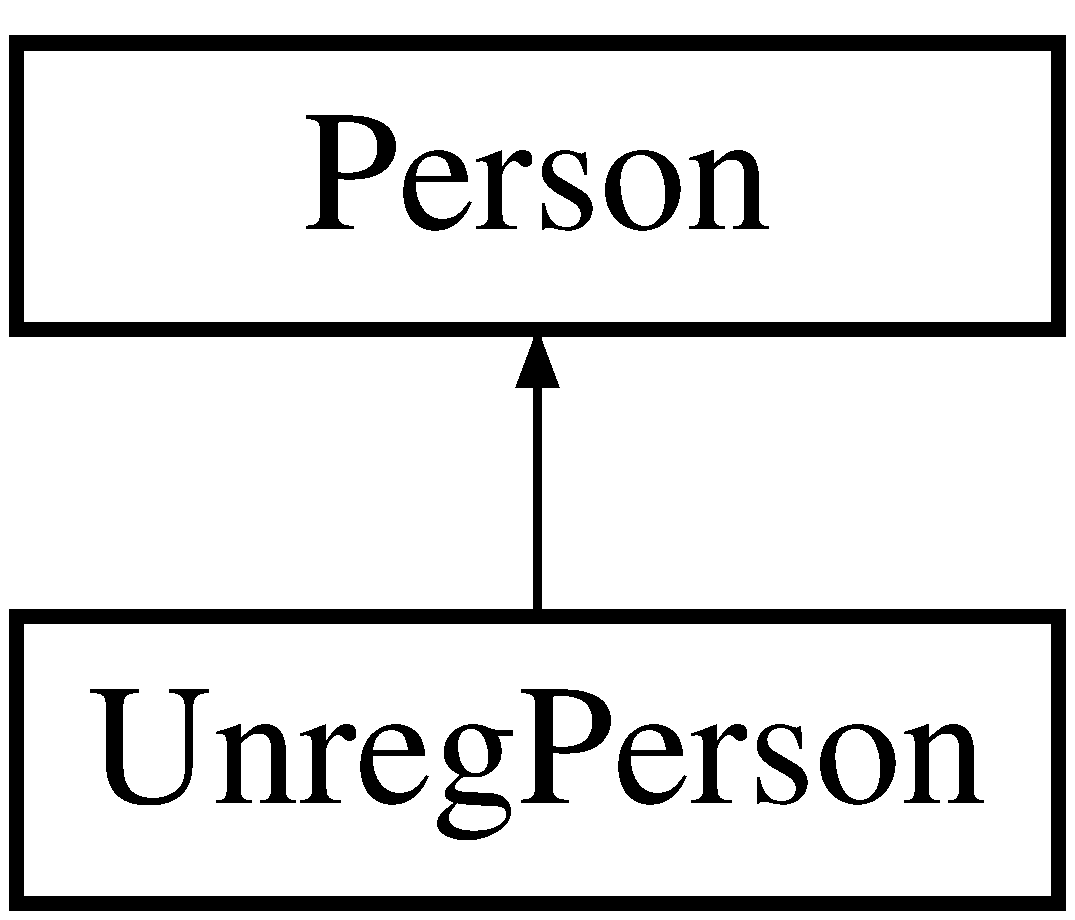
\includegraphics[height=2.000000cm]{class_unreg_person}
\end{center}
\end{figure}
\subsection*{Public Member Functions}
\begin{DoxyCompactItemize}
\item 
\hypertarget{class_unreg_person_aad823e6b15b4ef978f392f3d1714d0ad}{\hyperlink{class_unreg_person_aad823e6b15b4ef978f392f3d1714d0ad}{Unreg\+Person} ()}\label{class_unreg_person_aad823e6b15b4ef978f392f3d1714d0ad}

\begin{DoxyCompactList}\small\item\em \hyperlink{class_unreg_person}{Unreg\+Person} default constructor. \end{DoxyCompactList}\item 
\hyperlink{class_unreg_person_a2e072d7ef58345753feefabf26ae0faa}{Unreg\+Person} (string n, unsigned long t\+\_\+nr)
\begin{DoxyCompactList}\small\item\em \hyperlink{class_unreg_person}{Unreg\+Person} constructor. \end{DoxyCompactList}\item 
\hypertarget{class_unreg_person_a2a82cf4f0c01024b7a68c1d54a4d8ddc}{\hyperlink{class_unreg_person_a2a82cf4f0c01024b7a68c1d54a4d8ddc}{$\sim$\+Unreg\+Person} ()}\label{class_unreg_person_a2a82cf4f0c01024b7a68c1d54a4d8ddc}

\begin{DoxyCompactList}\small\item\em \hyperlink{class_unreg_person}{Unreg\+Person} destructor. \end{DoxyCompactList}\item 
void \hyperlink{class_unreg_person_aca26fc79ba28e05a1311659aea665d91}{add\+Bill} (string fee, float triplength)
\begin{DoxyCompactList}\small\item\em Adds bill to billing of unregistered person. \end{DoxyCompactList}\item 
\hypertarget{class_unreg_person_a72c5a1dff2af67a6b9b8eebb5f063f16}{void {\bfseries add\+Trip\+History} (\hyperlink{class_trip}{Trip} $\ast$t)}\label{class_unreg_person_a72c5a1dff2af67a6b9b8eebb5f063f16}

\item 
\hypertarget{class_unreg_person_a03234c8f6fa2860c4d104586f6d5ac49}{string {\bfseries get\+Usern} () const }\label{class_unreg_person_a03234c8f6fa2860c4d104586f6d5ac49}

\item 
\hypertarget{class_unreg_person_afdf29aaf8d484aa79c5f45f79b966d49}{void \hyperlink{class_unreg_person_afdf29aaf8d484aa79c5f45f79b966d49}{print\+Person} ()}\label{class_unreg_person_afdf29aaf8d484aa79c5f45f79b966d49}

\begin{DoxyCompactList}\small\item\em Prints unregistered person's information. \end{DoxyCompactList}\end{DoxyCompactItemize}
\subsection*{Additional Inherited Members}


\subsection{Detailed Description}
\hyperlink{class_unreg_person}{Unreg\+Person} class. 

\hyperlink{class_person}{Person} subclass, represents unregistered users in the application 

\subsection{Constructor \& Destructor Documentation}
\hypertarget{class_unreg_person_a2e072d7ef58345753feefabf26ae0faa}{\index{Unreg\+Person@{Unreg\+Person}!Unreg\+Person@{Unreg\+Person}}
\index{Unreg\+Person@{Unreg\+Person}!Unreg\+Person@{Unreg\+Person}}
\subsubsection[{Unreg\+Person}]{\setlength{\rightskip}{0pt plus 5cm}Unreg\+Person\+::\+Unreg\+Person (
\begin{DoxyParamCaption}
\item[{string}]{n, }
\item[{unsigned long}]{t\+\_\+nr}
\end{DoxyParamCaption}
)}}\label{class_unreg_person_a2e072d7ef58345753feefabf26ae0faa}


\hyperlink{class_unreg_person}{Unreg\+Person} constructor. 


\begin{DoxyParams}{Parameters}
{\em n} & name of unregistered person \\
\hline
{\em t\+\_\+nr} & phone number of unregistered person \\
\hline
\end{DoxyParams}


\subsection{Member Function Documentation}
\hypertarget{class_unreg_person_aca26fc79ba28e05a1311659aea665d91}{\index{Unreg\+Person@{Unreg\+Person}!add\+Bill@{add\+Bill}}
\index{add\+Bill@{add\+Bill}!Unreg\+Person@{Unreg\+Person}}
\subsubsection[{add\+Bill}]{\setlength{\rightskip}{0pt plus 5cm}void Unreg\+Person\+::add\+Bill (
\begin{DoxyParamCaption}
\item[{string}]{fee, }
\item[{float}]{triplength}
\end{DoxyParamCaption}
)\hspace{0.3cm}{\ttfamily [virtual]}}}\label{class_unreg_person_aca26fc79ba28e05a1311659aea665d91}


Adds bill to billing of unregistered person. 


\begin{DoxyParams}{Parameters}
{\em string} & fee -\/ what kind of fee to charge \\
\hline
{\em float} & triplength -\/ distance of the trip produces higher charges \\
\hline
\end{DoxyParams}


Reimplemented from \hyperlink{class_person}{Person}.



The documentation for this class was generated from the following files\+:\begin{DoxyCompactItemize}
\item 
Person.\+h\item 
Person.\+cpp\end{DoxyCompactItemize}

\hypertarget{class_vehicle}{\section{Vehicle Class Reference}
\label{class_vehicle}\index{Vehicle@{Vehicle}}
}


\hyperlink{class_vehicle}{Vehicle} class.  




{\ttfamily \#include $<$Vehicle.\+h$>$}

\subsection*{Public Member Functions}
\begin{DoxyCompactItemize}
\item 
\hypertarget{class_vehicle_abaad8187d9f2ede4fb8ea18de0a6764c}{\hyperlink{class_vehicle_abaad8187d9f2ede4fb8ea18de0a6764c}{Vehicle} ()}\label{class_vehicle_abaad8187d9f2ede4fb8ea18de0a6764c}

\begin{DoxyCompactList}\small\item\em \hyperlink{class_vehicle}{Vehicle} default constructor. \end{DoxyCompactList}\item 
\hyperlink{class_vehicle_a95edd9343b3e76eade8df5a44be799e5}{Vehicle} (string o, string t, string b, string l\+\_\+p, unsigned int c\+\_\+s)
\begin{DoxyCompactList}\small\item\em \hyperlink{class_vehicle}{Vehicle} constructor. \end{DoxyCompactList}\item 
\hypertarget{class_vehicle_a61ab140c755b8e0e824d54117cf4546f}{\hyperlink{class_vehicle_a61ab140c755b8e0e824d54117cf4546f}{$\sim$\+Vehicle} ()}\label{class_vehicle_a61ab140c755b8e0e824d54117cf4546f}

\begin{DoxyCompactList}\small\item\em \hyperlink{class_vehicle}{Vehicle} default destructor. \end{DoxyCompactList}\item 
void \hyperlink{class_vehicle_ad39892e6ee302c039e06c3e629802d0f}{set\+Owner} (string o)
\begin{DoxyCompactList}\small\item\em Sets the vehicle's owner name. \end{DoxyCompactList}\item 
void \hyperlink{class_vehicle_a344f7cc363febf23d205877b544efef8}{set\+Type} (string t)
\begin{DoxyCompactList}\small\item\em Sets the vehicle's type. \end{DoxyCompactList}\item 
void \hyperlink{class_vehicle_af8466ac38dc2d48a1d65b8037b667d6b}{set\+Brand} (string b)
\begin{DoxyCompactList}\small\item\em Sets the vehicle's brand. \end{DoxyCompactList}\item 
void \hyperlink{class_vehicle_a048147fc584afa2bcb7abed044476a3c}{set\+License\+Plate} (string l\+\_\+p)
\begin{DoxyCompactList}\small\item\em Sets the vehicle's license plate. \end{DoxyCompactList}\item 
void \hyperlink{class_vehicle_ae5b5d36f539e0fad3d37466ffa2ec9dc}{set\+Car\+Seats} (unsigned int c\+\_\+s)
\begin{DoxyCompactList}\small\item\em Sets the vehicle's seats. \end{DoxyCompactList}\item 
string \hyperlink{class_vehicle_a02d081f322381db9695e30aa5bb4116b}{get\+Owner} () const 
\begin{DoxyCompactList}\small\item\em Returns the name of the owner. \end{DoxyCompactList}\item 
string \hyperlink{class_vehicle_ab3c3d57639bae4a51ea193582e26c5e7}{get\+Type} () const 
\begin{DoxyCompactList}\small\item\em Returns the type of the vehicle. \end{DoxyCompactList}\item 
string \hyperlink{class_vehicle_a7c479d1f5be8a00a1e765345e1e2bf13}{get\+Brand} () const 
\begin{DoxyCompactList}\small\item\em Returns the vehicle's brand. \end{DoxyCompactList}\item 
string \hyperlink{class_vehicle_a70ea176477f0552924460029e6077708}{get\+License\+Plate} () const 
\begin{DoxyCompactList}\small\item\em Returns the vehicle's license plate. \end{DoxyCompactList}\item 
unsigned int \hyperlink{class_vehicle_ad64b4f6e3fa9f215354c78a5bb74dd5c}{get\+Car\+Seats} () const 
\begin{DoxyCompactList}\small\item\em Returns the number of car seats. \end{DoxyCompactList}\item 
string \hyperlink{class_vehicle_abd9381537867c1a98430ab06ce51898f}{to\+String} ()
\begin{DoxyCompactList}\small\item\em Writes all the information about a vehicle to a string. \end{DoxyCompactList}\end{DoxyCompactItemize}


\subsection{Detailed Description}
\hyperlink{class_vehicle}{Vehicle} class. 

Contains the vehicle related functions, including getters, setters and to\+String functions. 

\subsection{Constructor \& Destructor Documentation}
\hypertarget{class_vehicle_a95edd9343b3e76eade8df5a44be799e5}{\index{Vehicle@{Vehicle}!Vehicle@{Vehicle}}
\index{Vehicle@{Vehicle}!Vehicle@{Vehicle}}
\subsubsection[{Vehicle}]{\setlength{\rightskip}{0pt plus 5cm}Vehicle\+::\+Vehicle (
\begin{DoxyParamCaption}
\item[{string}]{o, }
\item[{string}]{t, }
\item[{string}]{b, }
\item[{string}]{l\+\_\+p, }
\item[{unsigned int}]{c\+\_\+s}
\end{DoxyParamCaption}
)}}\label{class_vehicle_a95edd9343b3e76eade8df5a44be799e5}


\hyperlink{class_vehicle}{Vehicle} constructor. 


\begin{DoxyParams}{Parameters}
{\em o} & owner's name \\
\hline
{\em t} & vehicle's type \\
\hline
{\em b} & vehicle's brand \\
\hline
{\em b} & vehicle's license plate \\
\hline
{\em c\+\_\+s} & car seats of vehicle \\
\hline
\end{DoxyParams}


\subsection{Member Function Documentation}
\hypertarget{class_vehicle_a7c479d1f5be8a00a1e765345e1e2bf13}{\index{Vehicle@{Vehicle}!get\+Brand@{get\+Brand}}
\index{get\+Brand@{get\+Brand}!Vehicle@{Vehicle}}
\subsubsection[{get\+Brand}]{\setlength{\rightskip}{0pt plus 5cm}string Vehicle\+::get\+Brand (
\begin{DoxyParamCaption}
{}
\end{DoxyParamCaption}
) const}}\label{class_vehicle_a7c479d1f5be8a00a1e765345e1e2bf13}


Returns the vehicle's brand. 

\begin{DoxyReturn}{Returns}
string with the vehicle's brand 
\end{DoxyReturn}
\hypertarget{class_vehicle_ad64b4f6e3fa9f215354c78a5bb74dd5c}{\index{Vehicle@{Vehicle}!get\+Car\+Seats@{get\+Car\+Seats}}
\index{get\+Car\+Seats@{get\+Car\+Seats}!Vehicle@{Vehicle}}
\subsubsection[{get\+Car\+Seats}]{\setlength{\rightskip}{0pt plus 5cm}unsigned int Vehicle\+::get\+Car\+Seats (
\begin{DoxyParamCaption}
{}
\end{DoxyParamCaption}
) const}}\label{class_vehicle_ad64b4f6e3fa9f215354c78a5bb74dd5c}


Returns the number of car seats. 

\begin{DoxyReturn}{Returns}
unsigned int with the number of car seats 
\end{DoxyReturn}
\hypertarget{class_vehicle_a70ea176477f0552924460029e6077708}{\index{Vehicle@{Vehicle}!get\+License\+Plate@{get\+License\+Plate}}
\index{get\+License\+Plate@{get\+License\+Plate}!Vehicle@{Vehicle}}
\subsubsection[{get\+License\+Plate}]{\setlength{\rightskip}{0pt plus 5cm}string Vehicle\+::get\+License\+Plate (
\begin{DoxyParamCaption}
{}
\end{DoxyParamCaption}
) const}}\label{class_vehicle_a70ea176477f0552924460029e6077708}


Returns the vehicle's license plate. 

\begin{DoxyReturn}{Returns}
string with the license plate 
\end{DoxyReturn}
\hypertarget{class_vehicle_a02d081f322381db9695e30aa5bb4116b}{\index{Vehicle@{Vehicle}!get\+Owner@{get\+Owner}}
\index{get\+Owner@{get\+Owner}!Vehicle@{Vehicle}}
\subsubsection[{get\+Owner}]{\setlength{\rightskip}{0pt plus 5cm}string Vehicle\+::get\+Owner (
\begin{DoxyParamCaption}
{}
\end{DoxyParamCaption}
) const}}\label{class_vehicle_a02d081f322381db9695e30aa5bb4116b}


Returns the name of the owner. 

\begin{DoxyReturn}{Returns}
string with the owner's name 
\end{DoxyReturn}
\hypertarget{class_vehicle_ab3c3d57639bae4a51ea193582e26c5e7}{\index{Vehicle@{Vehicle}!get\+Type@{get\+Type}}
\index{get\+Type@{get\+Type}!Vehicle@{Vehicle}}
\subsubsection[{get\+Type}]{\setlength{\rightskip}{0pt plus 5cm}string Vehicle\+::get\+Type (
\begin{DoxyParamCaption}
{}
\end{DoxyParamCaption}
) const}}\label{class_vehicle_ab3c3d57639bae4a51ea193582e26c5e7}


Returns the type of the vehicle. 

\begin{DoxyReturn}{Returns}
string with the vehicle's type 
\end{DoxyReturn}
\hypertarget{class_vehicle_af8466ac38dc2d48a1d65b8037b667d6b}{\index{Vehicle@{Vehicle}!set\+Brand@{set\+Brand}}
\index{set\+Brand@{set\+Brand}!Vehicle@{Vehicle}}
\subsubsection[{set\+Brand}]{\setlength{\rightskip}{0pt plus 5cm}void Vehicle\+::set\+Brand (
\begin{DoxyParamCaption}
\item[{string}]{b}
\end{DoxyParamCaption}
)}}\label{class_vehicle_af8466ac38dc2d48a1d65b8037b667d6b}


Sets the vehicle's brand. 


\begin{DoxyParams}{Parameters}
{\em t} & string with the vehicle's brand \\
\hline
\end{DoxyParams}
\hypertarget{class_vehicle_ae5b5d36f539e0fad3d37466ffa2ec9dc}{\index{Vehicle@{Vehicle}!set\+Car\+Seats@{set\+Car\+Seats}}
\index{set\+Car\+Seats@{set\+Car\+Seats}!Vehicle@{Vehicle}}
\subsubsection[{set\+Car\+Seats}]{\setlength{\rightskip}{0pt plus 5cm}void Vehicle\+::set\+Car\+Seats (
\begin{DoxyParamCaption}
\item[{unsigned int}]{c\+\_\+s}
\end{DoxyParamCaption}
)}}\label{class_vehicle_ae5b5d36f539e0fad3d37466ffa2ec9dc}


Sets the vehicle's seats. 


\begin{DoxyParams}{Parameters}
{\em c\+\_\+s} & unsigned int with the vehicle's seats. \\
\hline
\end{DoxyParams}
\hypertarget{class_vehicle_a048147fc584afa2bcb7abed044476a3c}{\index{Vehicle@{Vehicle}!set\+License\+Plate@{set\+License\+Plate}}
\index{set\+License\+Plate@{set\+License\+Plate}!Vehicle@{Vehicle}}
\subsubsection[{set\+License\+Plate}]{\setlength{\rightskip}{0pt plus 5cm}void Vehicle\+::set\+License\+Plate (
\begin{DoxyParamCaption}
\item[{string}]{l\+\_\+p}
\end{DoxyParamCaption}
)}}\label{class_vehicle_a048147fc584afa2bcb7abed044476a3c}


Sets the vehicle's license plate. 


\begin{DoxyParams}{Parameters}
{\em l\+\_\+p} & string with the vehicle's license\+\_\+plate \\
\hline
\end{DoxyParams}
\hypertarget{class_vehicle_ad39892e6ee302c039e06c3e629802d0f}{\index{Vehicle@{Vehicle}!set\+Owner@{set\+Owner}}
\index{set\+Owner@{set\+Owner}!Vehicle@{Vehicle}}
\subsubsection[{set\+Owner}]{\setlength{\rightskip}{0pt plus 5cm}void Vehicle\+::set\+Owner (
\begin{DoxyParamCaption}
\item[{string}]{o}
\end{DoxyParamCaption}
)}}\label{class_vehicle_ad39892e6ee302c039e06c3e629802d0f}


Sets the vehicle's owner name. 


\begin{DoxyParams}{Parameters}
{\em o} & string with the owner's name \\
\hline
\end{DoxyParams}
\hypertarget{class_vehicle_a344f7cc363febf23d205877b544efef8}{\index{Vehicle@{Vehicle}!set\+Type@{set\+Type}}
\index{set\+Type@{set\+Type}!Vehicle@{Vehicle}}
\subsubsection[{set\+Type}]{\setlength{\rightskip}{0pt plus 5cm}void Vehicle\+::set\+Type (
\begin{DoxyParamCaption}
\item[{string}]{t}
\end{DoxyParamCaption}
)}}\label{class_vehicle_a344f7cc363febf23d205877b544efef8}


Sets the vehicle's type. 


\begin{DoxyParams}{Parameters}
{\em t} & string with the vehicle's type \\
\hline
\end{DoxyParams}
\hypertarget{class_vehicle_abd9381537867c1a98430ab06ce51898f}{\index{Vehicle@{Vehicle}!to\+String@{to\+String}}
\index{to\+String@{to\+String}!Vehicle@{Vehicle}}
\subsubsection[{to\+String}]{\setlength{\rightskip}{0pt plus 5cm}string Vehicle\+::to\+String (
\begin{DoxyParamCaption}
{}
\end{DoxyParamCaption}
)}}\label{class_vehicle_abd9381537867c1a98430ab06ce51898f}


Writes all the information about a vehicle to a string. 

\begin{DoxyReturn}{Returns}
string with the vehicle's information 
\end{DoxyReturn}


The documentation for this class was generated from the following files\+:\begin{DoxyCompactItemize}
\item 
Vehicle.\+h\item 
Vehicle.\+cpp\end{DoxyCompactItemize}

%--- End generated contents ---

% Index
\newpage
\phantomsection
\addcontentsline{toc}{chapter}{Index}
\printindex

\end{document}
